% Options for packages loaded elsewhere
\PassOptionsToPackage{unicode}{hyperref}
\PassOptionsToPackage{hyphens}{url}
\PassOptionsToPackage{dvipsnames,svgnames,x11names}{xcolor}
%
\documentclass[
  letterpaper,
  DIV=11,
  numbers=noendperiod]{scrreprt}

\usepackage{amsmath,amssymb}
\usepackage{iftex}
\ifPDFTeX
  \usepackage[T1]{fontenc}
  \usepackage[utf8]{inputenc}
  \usepackage{textcomp} % provide euro and other symbols
\else % if luatex or xetex
  \usepackage{unicode-math}
  \defaultfontfeatures{Scale=MatchLowercase}
  \defaultfontfeatures[\rmfamily]{Ligatures=TeX,Scale=1}
\fi
\usepackage{lmodern}
\ifPDFTeX\else  
    % xetex/luatex font selection
\fi
% Use upquote if available, for straight quotes in verbatim environments
\IfFileExists{upquote.sty}{\usepackage{upquote}}{}
\IfFileExists{microtype.sty}{% use microtype if available
  \usepackage[]{microtype}
  \UseMicrotypeSet[protrusion]{basicmath} % disable protrusion for tt fonts
}{}
\makeatletter
\@ifundefined{KOMAClassName}{% if non-KOMA class
  \IfFileExists{parskip.sty}{%
    \usepackage{parskip}
  }{% else
    \setlength{\parindent}{0pt}
    \setlength{\parskip}{6pt plus 2pt minus 1pt}}
}{% if KOMA class
  \KOMAoptions{parskip=half}}
\makeatother
\usepackage{xcolor}
\setlength{\emergencystretch}{3em} % prevent overfull lines
\setcounter{secnumdepth}{5}
% Make \paragraph and \subparagraph free-standing
\ifx\paragraph\undefined\else
  \let\oldparagraph\paragraph
  \renewcommand{\paragraph}[1]{\oldparagraph{#1}\mbox{}}
\fi
\ifx\subparagraph\undefined\else
  \let\oldsubparagraph\subparagraph
  \renewcommand{\subparagraph}[1]{\oldsubparagraph{#1}\mbox{}}
\fi

\usepackage{color}
\usepackage{fancyvrb}
\newcommand{\VerbBar}{|}
\newcommand{\VERB}{\Verb[commandchars=\\\{\}]}
\DefineVerbatimEnvironment{Highlighting}{Verbatim}{commandchars=\\\{\}}
% Add ',fontsize=\small' for more characters per line
\usepackage{framed}
\definecolor{shadecolor}{RGB}{241,243,245}
\newenvironment{Shaded}{\begin{snugshade}}{\end{snugshade}}
\newcommand{\AlertTok}[1]{\textcolor[rgb]{0.68,0.00,0.00}{#1}}
\newcommand{\AnnotationTok}[1]{\textcolor[rgb]{0.37,0.37,0.37}{#1}}
\newcommand{\AttributeTok}[1]{\textcolor[rgb]{0.40,0.45,0.13}{#1}}
\newcommand{\BaseNTok}[1]{\textcolor[rgb]{0.68,0.00,0.00}{#1}}
\newcommand{\BuiltInTok}[1]{\textcolor[rgb]{0.00,0.23,0.31}{#1}}
\newcommand{\CharTok}[1]{\textcolor[rgb]{0.13,0.47,0.30}{#1}}
\newcommand{\CommentTok}[1]{\textcolor[rgb]{0.37,0.37,0.37}{#1}}
\newcommand{\CommentVarTok}[1]{\textcolor[rgb]{0.37,0.37,0.37}{\textit{#1}}}
\newcommand{\ConstantTok}[1]{\textcolor[rgb]{0.56,0.35,0.01}{#1}}
\newcommand{\ControlFlowTok}[1]{\textcolor[rgb]{0.00,0.23,0.31}{#1}}
\newcommand{\DataTypeTok}[1]{\textcolor[rgb]{0.68,0.00,0.00}{#1}}
\newcommand{\DecValTok}[1]{\textcolor[rgb]{0.68,0.00,0.00}{#1}}
\newcommand{\DocumentationTok}[1]{\textcolor[rgb]{0.37,0.37,0.37}{\textit{#1}}}
\newcommand{\ErrorTok}[1]{\textcolor[rgb]{0.68,0.00,0.00}{#1}}
\newcommand{\ExtensionTok}[1]{\textcolor[rgb]{0.00,0.23,0.31}{#1}}
\newcommand{\FloatTok}[1]{\textcolor[rgb]{0.68,0.00,0.00}{#1}}
\newcommand{\FunctionTok}[1]{\textcolor[rgb]{0.28,0.35,0.67}{#1}}
\newcommand{\ImportTok}[1]{\textcolor[rgb]{0.00,0.46,0.62}{#1}}
\newcommand{\InformationTok}[1]{\textcolor[rgb]{0.37,0.37,0.37}{#1}}
\newcommand{\KeywordTok}[1]{\textcolor[rgb]{0.00,0.23,0.31}{#1}}
\newcommand{\NormalTok}[1]{\textcolor[rgb]{0.00,0.23,0.31}{#1}}
\newcommand{\OperatorTok}[1]{\textcolor[rgb]{0.37,0.37,0.37}{#1}}
\newcommand{\OtherTok}[1]{\textcolor[rgb]{0.00,0.23,0.31}{#1}}
\newcommand{\PreprocessorTok}[1]{\textcolor[rgb]{0.68,0.00,0.00}{#1}}
\newcommand{\RegionMarkerTok}[1]{\textcolor[rgb]{0.00,0.23,0.31}{#1}}
\newcommand{\SpecialCharTok}[1]{\textcolor[rgb]{0.37,0.37,0.37}{#1}}
\newcommand{\SpecialStringTok}[1]{\textcolor[rgb]{0.13,0.47,0.30}{#1}}
\newcommand{\StringTok}[1]{\textcolor[rgb]{0.13,0.47,0.30}{#1}}
\newcommand{\VariableTok}[1]{\textcolor[rgb]{0.07,0.07,0.07}{#1}}
\newcommand{\VerbatimStringTok}[1]{\textcolor[rgb]{0.13,0.47,0.30}{#1}}
\newcommand{\WarningTok}[1]{\textcolor[rgb]{0.37,0.37,0.37}{\textit{#1}}}

\providecommand{\tightlist}{%
  \setlength{\itemsep}{0pt}\setlength{\parskip}{0pt}}\usepackage{longtable,booktabs,array}
\usepackage{calc} % for calculating minipage widths
% Correct order of tables after \paragraph or \subparagraph
\usepackage{etoolbox}
\makeatletter
\patchcmd\longtable{\par}{\if@noskipsec\mbox{}\fi\par}{}{}
\makeatother
% Allow footnotes in longtable head/foot
\IfFileExists{footnotehyper.sty}{\usepackage{footnotehyper}}{\usepackage{footnote}}
\makesavenoteenv{longtable}
\usepackage{graphicx}
\makeatletter
\def\maxwidth{\ifdim\Gin@nat@width>\linewidth\linewidth\else\Gin@nat@width\fi}
\def\maxheight{\ifdim\Gin@nat@height>\textheight\textheight\else\Gin@nat@height\fi}
\makeatother
% Scale images if necessary, so that they will not overflow the page
% margins by default, and it is still possible to overwrite the defaults
% using explicit options in \includegraphics[width, height, ...]{}
\setkeys{Gin}{width=\maxwidth,height=\maxheight,keepaspectratio}
% Set default figure placement to htbp
\makeatletter
\def\fps@figure{htbp}
\makeatother

\KOMAoption{captions}{tableheading}
\makeatletter
\@ifpackageloaded{bookmark}{}{\usepackage{bookmark}}
\makeatother
\makeatletter
\@ifpackageloaded{caption}{}{\usepackage{caption}}
\AtBeginDocument{%
\ifdefined\contentsname
  \renewcommand*\contentsname{Table of contents}
\else
  \newcommand\contentsname{Table of contents}
\fi
\ifdefined\listfigurename
  \renewcommand*\listfigurename{List of Figures}
\else
  \newcommand\listfigurename{List of Figures}
\fi
\ifdefined\listtablename
  \renewcommand*\listtablename{List of Tables}
\else
  \newcommand\listtablename{List of Tables}
\fi
\ifdefined\figurename
  \renewcommand*\figurename{Figure}
\else
  \newcommand\figurename{Figure}
\fi
\ifdefined\tablename
  \renewcommand*\tablename{Table}
\else
  \newcommand\tablename{Table}
\fi
}
\@ifpackageloaded{float}{}{\usepackage{float}}
\floatstyle{ruled}
\@ifundefined{c@chapter}{\newfloat{codelisting}{h}{lop}}{\newfloat{codelisting}{h}{lop}[chapter]}
\floatname{codelisting}{Listing}
\newcommand*\listoflistings{\listof{codelisting}{List of Listings}}
\makeatother
\makeatletter
\makeatother
\makeatletter
\@ifpackageloaded{caption}{}{\usepackage{caption}}
\@ifpackageloaded{subcaption}{}{\usepackage{subcaption}}
\makeatother
\ifLuaTeX
  \usepackage{selnolig}  % disable illegal ligatures
\fi
\usepackage{bookmark}

\IfFileExists{xurl.sty}{\usepackage{xurl}}{} % add URL line breaks if available
\urlstyle{same} % disable monospaced font for URLs
\hypersetup{
  pdftitle={COMP/STAT 112: Introduction to Data Science},
  colorlinks=true,
  linkcolor={blue},
  filecolor={Maroon},
  citecolor={Blue},
  urlcolor={Blue},
  pdfcreator={LaTeX via pandoc}}

\title{COMP/STAT 112: Introduction to Data Science}
\author{}
\date{}

\begin{document}
\maketitle

\renewcommand*\contentsname{Table of contents}
{
\hypersetup{linkcolor=}
\setcounter{tocdepth}{2}
\tableofcontents
}
\bookmarksetup{startatroot}

\chapter*{Welcome}\label{welcome}
\addcontentsline{toc}{chapter}{Welcome}

\markboth{Welcome}{Welcome}

\part{Foundation}

\chapter{Intro to R, RStudio, and R
Markdown}\label{intro-to-r-rstudio-and-r-markdown}

\section{Learning Goals}\label{learning-goals}

\begin{itemize}
\tightlist
\item
  Download and install the necessary tools (R, RStudio)
\item
  Develop comfort in navigating the tools in RStudio
\item
  Develop comfort in writing and knitting a R Markdown (or a new Quarto)
  file
\item
  Identify the characteristics of tidy data
\item
  Use R code: as a calculator and to explore tidy data
\end{itemize}

\section{Getting Started in RStudio}\label{getting-started-in-rstudio}

As you might guess from the name, ``Data Science'' requires \emph{data}.
Working with modern (large, messy) data sets requires statistical
software. We'll exclusively use \textbf{RStudio}. Why?

\begin{itemize}
\tightlist
\item
  it's free\\
\item
  it's open source (the code is free \& anybody can contribute to it)
\item
  it has a huge online community (which is helpful for when you get
  stuck)\\
\item
  it's one of the industry standards\\
\item
  it can be used to create \emph{reproducible} and lovely documents (In
  fact, the course materials that you're currently reading were
  constructed entirely within RStudio!)
\end{itemize}

\subsection{Download R \& RStudio}\label{download-r-rstudio}

To get started, take the following two steps \emph{in the given order}.
Even if you already have R/RStudio, make sure to update to the most
recent versions.

\begin{enumerate}
\def\labelenumi{\arabic{enumi}.}
\tightlist
\item
  Download and install the R statistical software at
  \url{https://mirror.las.iastate.edu/CRAN/}\\
\end{enumerate}

\begin{itemize}
\tightlist
\item
  Mac: Check to see if you have an Intel or Apple Silicon Processor Chip
  (Apple logo \textgreater{} About this Mac). This will impact the
  version you download.
\end{itemize}

\begin{enumerate}
\def\labelenumi{\arabic{enumi}.}
\setcounter{enumi}{1}
\tightlist
\item
  Download and install the FREE version of RStudio at
  \url{https://posit.co/download/rstudio-desktop/}
\end{enumerate}

\begin{itemize}
\tightlist
\item
  Mac: Once you download the dmg file and click on it, drag the RStudio
  icon to applications and then open Finder and click the eject icon
  next to the RStudio temporary drive under Locations.
\end{itemize}

If you are having issues with downloading, log on to
\url{https://rstudio.macalester.edu/} (use Mac credentials) to use the
RStudio server.

What's the difference between R and RStudio? Mainly, RStudio requires R
-- thus it does everything R does \emph{and more}. We will be using
RStudio exclusively.

\subsection{A quick tour of RStudio}\label{a-quick-tour-of-rstudio}

Open RStudio! You should see four panes, each serving a different
purpose:

\begin{figure}

\centering{

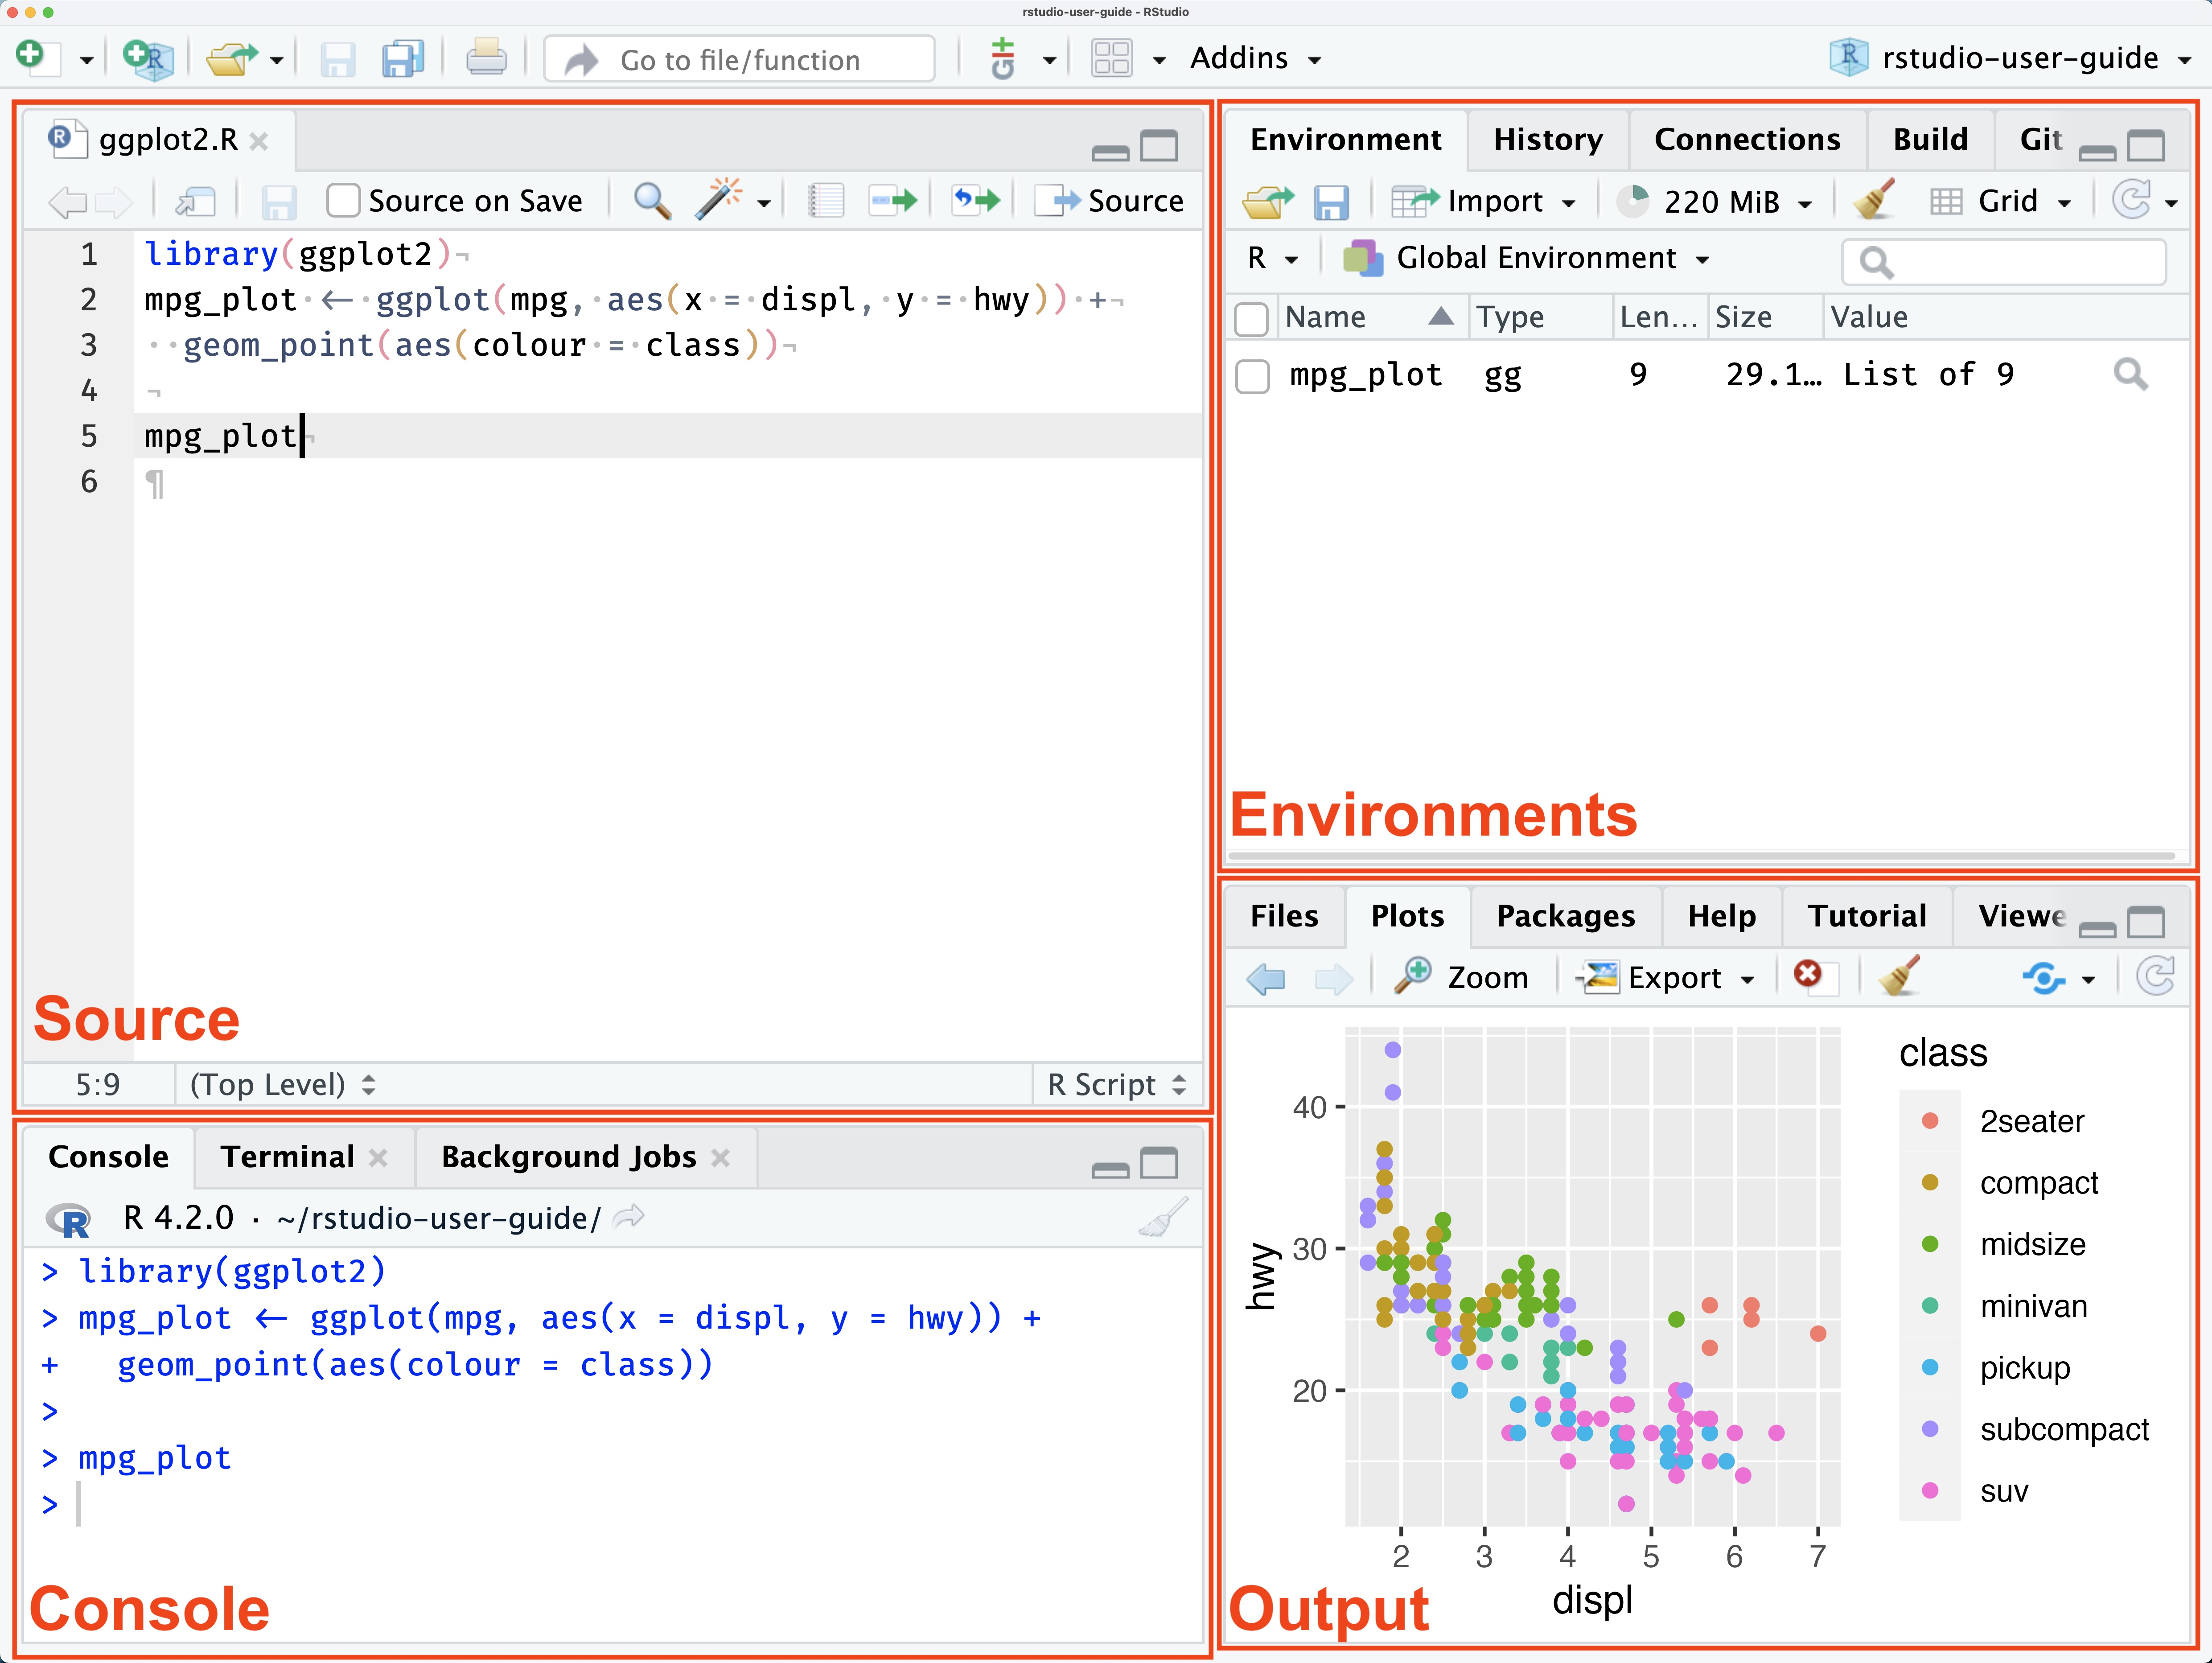
\includegraphics[width=16.54in,height=\textheight]{src/../images/rstudio-panes-labeled.jpeg}

}

\caption{\label{fig-main}RStudio Interface}

\end{figure}%

This short \href{http://www.youtube.com/embed/JfIo2Ua_oqQ/}{video tour
of RStudio} summarizes some basic features of the \emph{console}.

\begin{verbatim}
Use RStudio as a simple calculator to do the following:
  
  1) Perform a simple calculation: calculate `90/3`.
  2) RStudio has built-in *functions* to which we supply the necessary *arguments*:  `function(arguments)`.  Use the built-in function `sqrt` to calculate the square root of 25.
  3) Use the built-in function `rep` to repeat the number "5" eight times. (Type `?rep` in the console and press Return. Check out the Help documentation for examples at the bottom.)
  4) Use the `seq` function to create the vector `(0, 3, 6, 9, 12)`.  (Type `?seq` in the console and press Return.)
  5) Create a new vector by concatenating three repetitions of the vector from the previous part. (Type `?c` in the console and press Return.)
\end{verbatim}

Solution

\begin{Shaded}
\begin{Highlighting}[]
\DecValTok{90}\SpecialCharTok{/}\DecValTok{3} 
\DocumentationTok{\#\# [1] 30}

\FunctionTok{sqrt}\NormalTok{(}\DecValTok{25}\NormalTok{)}
\DocumentationTok{\#\# [1] 5}

\FunctionTok{rep}\NormalTok{(}\DecValTok{5}\NormalTok{, }\AttributeTok{times =} \DecValTok{8}\NormalTok{)}
\DocumentationTok{\#\# [1] 5 5 5 5 5 5 5 5}

\FunctionTok{seq}\NormalTok{(}\DecValTok{0}\NormalTok{, }\DecValTok{12}\NormalTok{, }\AttributeTok{by =} \DecValTok{3}\NormalTok{)}
\DocumentationTok{\#\# [1]  0  3  6  9 12}

\FunctionTok{rep}\NormalTok{(}\FunctionTok{seq}\NormalTok{(}\DecValTok{0}\NormalTok{, }\DecValTok{12}\NormalTok{, }\AttributeTok{by =} \DecValTok{3}\NormalTok{), }\AttributeTok{times =}  \DecValTok{3}\NormalTok{)}
\DocumentationTok{\#\#  [1]  0  3  6  9 12  0  3  6  9 12  0  3  6  9 12}

\FunctionTok{rep}\NormalTok{(}\FunctionTok{seq}\NormalTok{(}\DecValTok{0}\NormalTok{, }\DecValTok{12}\NormalTok{, }\AttributeTok{by =} \DecValTok{3}\NormalTok{), }\AttributeTok{each =} \DecValTok{3}\NormalTok{) }\CommentTok{\#notice the difference between the named input of times and each}
\DocumentationTok{\#\#  [1]  0  0  0  3  3  3  6  6  6  9  9  9 12 12 12}
\end{Highlighting}
\end{Shaded}

```\{name=``Assigning Values to Variables'', label=``assignment''\} We
often want to store our output for later use (why?). The basic idea in
R:

\begin{verbatim}
`name <- output`
\end{verbatim}

Copy and paste the following code into the console, line by line. NOTE:
RStudio ignores any content after the \texttt{\#}. Thus we use this to
make `comments' and organize our code.

\begin{verbatim}



::: {.cell}

```{.r .cell-code}
#type square_3
square_3
    
#calculate 3 squared
3^2    
    
#store this as "square_3"
square_3 <- 3^2    
    
#type square_3 again!
square_3
    
#do some math with square_3
square_3 + 2
\end{verbatim}

:::

\subsection{Data}\label{data}

Not only does ``Data Science'' require statistical software, it requires
\emph{DATA}! Consider the Google definition:

\begin{figure}[H]

{\centering 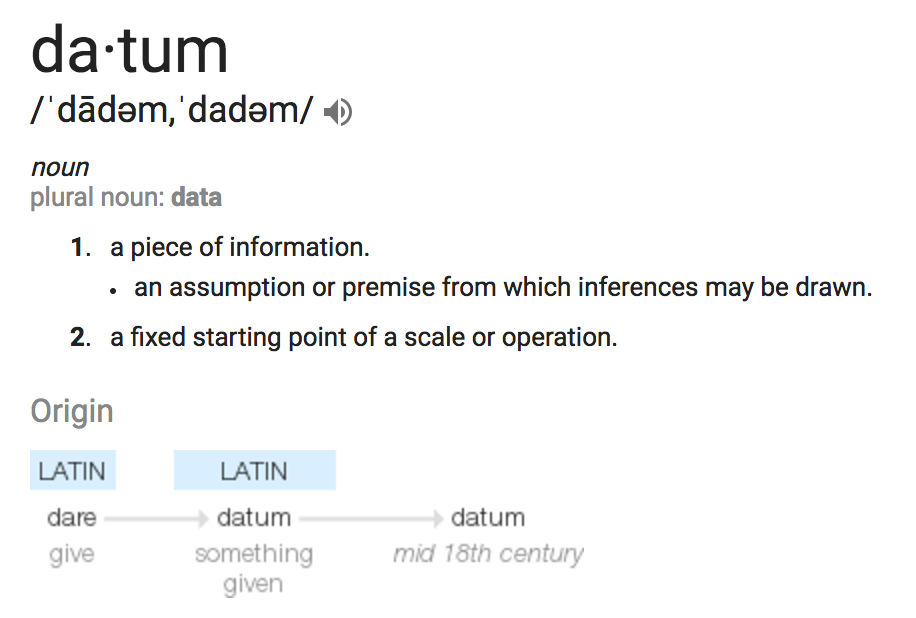
\includegraphics[width=3.05in,height=\textheight]{src/../images/datum.png}

}

\caption{A datum.}

\end{figure}%

With this definition in mind, which of the following are examples of
data?

\begin{itemize}
\tightlist
\item
  tables
\end{itemize}

\begin{verbatim}
  family father mother sex height nkids
1      1   78.5   67.0   M   73.2     4
2      1   78.5   67.0   F   69.2     4
3      1   78.5   67.0   F   69.0     4
4      1   78.5   67.0   F   69.0     4
5      2   75.5   66.5   M   73.5     4
6      2   75.5   66.5   M   72.5     4
\end{verbatim}

\begin{itemize}
\item
  \href{https://www.google.com/search?hl=en&biw=1439&bih=656&tbm=isch&sa=1&q=messy+college+dorm+rooms&oq=messy+college+dorm+rooms&gs_l=psy-ab.3...20720.21922.0.22183.6.6.0.0.0.0.143.552.4j2.6.0....0...1.1.64.psy-ab..1.1.142...0i13k1.uaj5gYQ4t50}{photo}
\item
  \href{https://www.youtube.com/watch?v=wMm7VdH05jY}{video}
\item
  \href{https://twitter.com/data4blacklives?lang=en}{text / tweets}
\end{itemize}

We'll mostly work with data that look like this:

\begin{verbatim}
  family father mother sex height nkids
1      1   78.5   67.0   M   73.2     4
2      1   78.5   67.0   F   69.2     4
3      1   78.5   67.0   F   69.0     4
4      1   78.5   67.0   F   69.0     4
5      2   75.5   66.5   M   73.5     4
6      2   75.5   66.5   M   72.5     4
\end{verbatim}

This isn't as restrictive as it seems. We can convert the above signals:
photos, videos, and text to a data table format!

\subsection{Tidy Data}\label{tidy-data}

\textbf{Example:} After a scandal among FIFA officials,
fivethirtyeight.com posted an analysis of FIFA viewership,
\href{https://fivethirtyeight.com/features/how-to-break-fifa/}{``How to
Break FIFA''}. Here's a snapshot of the data used in this article:

\begin{verbatim}
Warning: package 'knitr' was built under R version 4.4.1
\end{verbatim}

\begin{longtable}[]{@{}
  >{\raggedright\arraybackslash}p{(\columnwidth - 8\tabcolsep) * \real{0.1807}}
  >{\raggedright\arraybackslash}p{(\columnwidth - 8\tabcolsep) * \real{0.1687}}
  >{\raggedleft\arraybackslash}p{(\columnwidth - 8\tabcolsep) * \real{0.2048}}
  >{\raggedleft\arraybackslash}p{(\columnwidth - 8\tabcolsep) * \real{0.2169}}
  >{\raggedleft\arraybackslash}p{(\columnwidth - 8\tabcolsep) * \real{0.2289}}@{}}
\toprule\noalign{}
\begin{minipage}[b]{\linewidth}\raggedright
country
\end{minipage} & \begin{minipage}[b]{\linewidth}\raggedright
confederation
\end{minipage} & \begin{minipage}[b]{\linewidth}\raggedleft
population\_share
\end{minipage} & \begin{minipage}[b]{\linewidth}\raggedleft
tv\_audience\_share
\end{minipage} & \begin{minipage}[b]{\linewidth}\raggedleft
gdp\_weighted\_share
\end{minipage} \\
\midrule\noalign{}
\endhead
\bottomrule\noalign{}
\endlastfoot
United States & CONCACAF & 4.5 & 4.3 & 11.3 \\
Japan & AFC & 1.9 & 4.9 & 9.1 \\
China & AFC & 19.5 & 14.8 & 7.3 \\
Germany & UEFA & 1.2 & 2.9 & 6.3 \\
Brazil & CONMEBOL & 2.8 & 7.1 & 5.4 \\
United Kingdom & UEFA & 0.9 & 2.1 & 4.2 \\
Italy & UEFA & 0.9 & 2.1 & 4.0 \\
France & UEFA & 0.9 & 2.0 & 4.0 \\
Russia & UEFA & 2.1 & 3.1 & 3.5 \\
Spain & UEFA & 0.7 & 1.8 & 3.1 \\
\end{longtable}

The data table above is in \emph{tidy} format. \emph{Tidy} data tables
have three key features:

\begin{enumerate}
\def\labelenumi{\arabic{enumi}.}
\tightlist
\item
  Each row represents a \textbf{unit of observation} (also referred to
  as a case).\\
\item
  Each column represents a \textbf{variable} (ie. an attribute of the
  cases that can vary from case to case). Each variable is one of two
  types:\\
\end{enumerate}

\begin{itemize}
\tightlist
\item
  \textbf{quantitative} = numerical/numbers with units\\
\item
  \textbf{categorical} = discrete possibilities/categories\\
\end{itemize}

\begin{enumerate}
\def\labelenumi{\arabic{enumi}.}
\setcounter{enumi}{2}
\tightlist
\item
  Each entry contains a single data value; no analysis, summaries,
  footnotes, comments, etc., and only one value per cell
\end{enumerate}

\begin{figure}[H]

{\centering 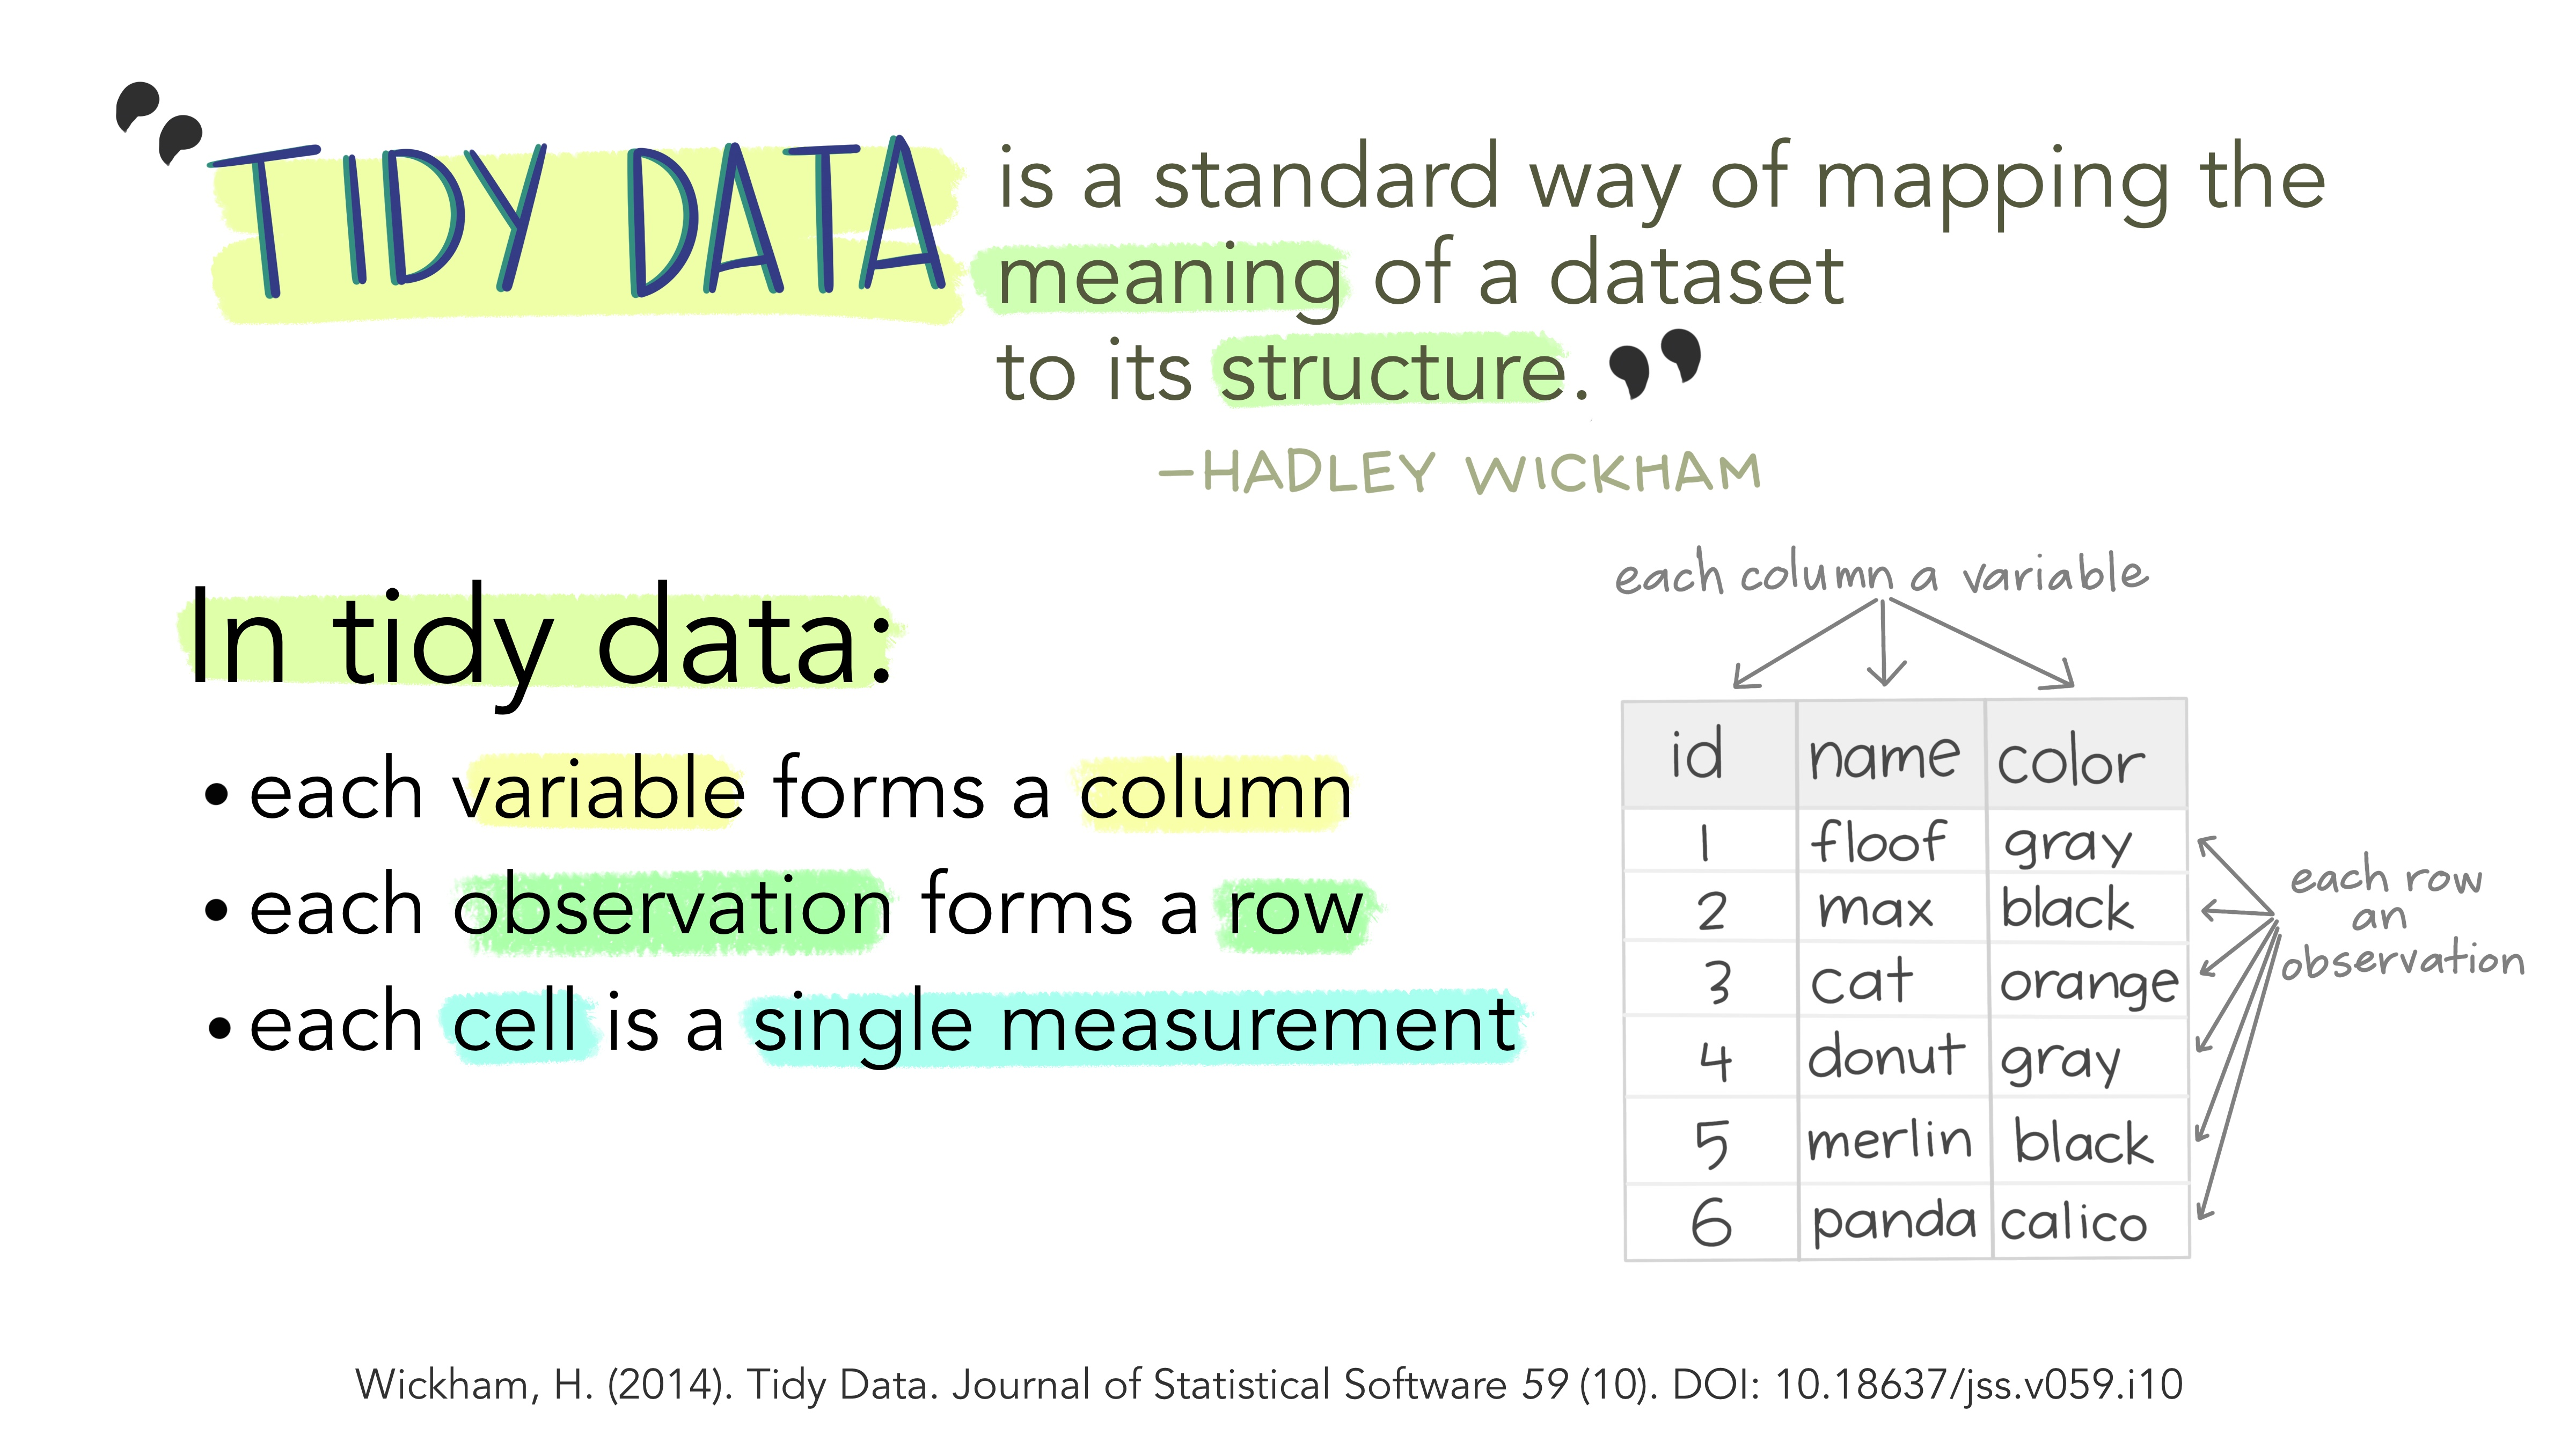
\includegraphics{src/../images/tidydata_1.jpg}

}

\caption{Tidy Data: Art by Allison Horst}

\end{figure}%

\begin{verbatim}
Consider the following in a group:   
\end{verbatim}

\begin{enumerate}
\def\labelenumi{\alph{enumi}.}
\tightlist
\item
  What are the units of observation in the FIFA data?\\
\item
  What are the variables? Which are quantitative? Which are
  categorical?\\
\item
  Are these \emph{tidy} data?
\end{enumerate}

Solution

\begin{enumerate}
\def\labelenumi{\alph{enumi}.}
\tightlist
\item
  A FIFA member country
\item
  country name, soccer or football confederation, country's share of
  global population (percentage), country's share of global world cup TV
  Audience (percentage), country's GDP-weighted audience share
  (percentage)
\item
  Yes
\end{enumerate}

\hfill\break

\begin{verbatim}
Check out the following data.  Explain to each other why they are untidy and how we can tidy them.    
  
  a. Data 1: FIFA    
    
              country  confederation  population share    tv_share
        ------------- -------------- ----------------- ----------- ------------------
        United States       CONCACAF     i don't know*       4.3%  *look up later      
                 Japan           AFC               1.9       4.9%
                 China           AFC              19.5      14.8%    
                                                        total=24%           
  
  b. Data 2: Gapminder life expectancies by country    
        
                          country  1952  1957  1962
        ------------ ------------ ----- ----- -----
                Asia  Afghanistan  28.8  30.3  32.0
                          Bahrain  50.9  53.8  56.9    
              Africa      Algeria  43.0  45.7  48.3    
\end{verbatim}

Solution

\begin{enumerate}
\def\labelenumi{\alph{enumi}.}
\tightlist
\item
  There are notes such as ``I don't know'' and ``look up later'' in
  columns with numeric values; the last row with the total is a summary.
  We could remove the text notes, replace it with the value if known,
  and remove the last row with the total summary.
\item
  The first column does not have a row name. It should be continent.
  Additionally, Bahrain needs a value for the continent.The column names
  `1952', `1957' and `1962' are values not variables. The table should
  be `pivoted' (more information on this coming soon!), so that there is
  an additional column named `year' and each country has three
  observations (rows) associated with it (one for each year).
\end{enumerate}

\subsection{Data Basics in RStudio}\label{data-basics-in-rstudio}

For now, we'll focus on \emph{tidy} data. In a couple of weeks, you'll
learn how to ``clean data'' and turn untidy data into tidy data.

\begin{verbatim}
The first step to working with data in RStudio is getting it in there!  How we do this depends on its format (eg: Excel spreadsheet, csv file, txt file) and storage locations (eg: online, within Wiki, desktop).  

Luckily for us, the `fifa_audience` data are stored in the `fivethirtyeight` RStudio package. Copy and paste the following code into the Console and press Enter.
\end{verbatim}

\begin{Shaded}
\begin{Highlighting}[]
\CommentTok{\#download the data and information in the fivethirtyeight package (we only need to do this once)}
\FunctionTok{install.packages}\NormalTok{(}\StringTok{\textquotesingle{}fivethirtyeight\textquotesingle{}}\NormalTok{)}

\CommentTok{\#load the fivethirtyeight package}
\FunctionTok{library}\NormalTok{(fivethirtyeight)}
    
\CommentTok{\#load the fifa data}
\FunctionTok{data}\NormalTok{(}\StringTok{"fifa\_audience"}\NormalTok{)}
    
\CommentTok{\#store this under a shorter, easier name}
\NormalTok{fifa }\OtherTok{\textless{}{-}}\NormalTok{ fifa\_audience}
\end{Highlighting}
\end{Shaded}

\begin{verbatim}
Before we can analyze our data, we must understand its structure.  Try out the following functions (copy and paste into the Console).  For each, make a note that describes its action.  
\end{verbatim}

\begin{Shaded}
\begin{Highlighting}[]
\CommentTok{\#(what does View do?)}
\FunctionTok{View}\NormalTok{(fifa)  }

\CommentTok{\#(what does head do?)}
\FunctionTok{head}\NormalTok{(fifa)  }

\CommentTok{\#(what does dim do?)}
\FunctionTok{dim}\NormalTok{(fifa)           }

\CommentTok{\#(what does names do?)}
\FunctionTok{names}\NormalTok{(fifa)         }
\end{Highlighting}
\end{Shaded}

Solution

\begin{Shaded}
\begin{Highlighting}[]
\CommentTok{\#View() opens up a new tab with a spreadsheet preview of the data to visually explore the data. It is commented out in the Rmarkdown/Quarto file because this is an interactive feature}
\CommentTok{\#View(fifa)  }

\CommentTok{\#head() gives the first 6 (default number) rows of a data set}
\FunctionTok{head}\NormalTok{(fifa)  }
\DocumentationTok{\#\# \# A tibble: 6 x 5}
\DocumentationTok{\#\#   country    confederation population\_share tv\_audience\_share gdp\_weighted\_share}
\DocumentationTok{\#\#   \textless{}chr\textgreater{}      \textless{}chr\textgreater{}                    \textless{}dbl\textgreater{}             \textless{}dbl\textgreater{}              \textless{}dbl\textgreater{}}
\DocumentationTok{\#\# 1 United St\textasciitilde{} CONCACAF                   4.5               4.3               11.3}
\DocumentationTok{\#\# 2 Japan      AFC                        1.9               4.9                9.1}
\DocumentationTok{\#\# 3 China      AFC                       19.5              14.8                7.3}
\DocumentationTok{\#\# 4 Germany    UEFA                       1.2               2.9                6.3}
\DocumentationTok{\#\# 5 Brazil     CONMEBOL                   2.8               7.1                5.4}
\DocumentationTok{\#\# 6 United Ki\textasciitilde{} UEFA                       0.9               2.1                4.2}

\CommentTok{\#dim() gives the number of rows and number of columns}
\FunctionTok{dim}\NormalTok{(fifa)           }
\DocumentationTok{\#\# [1] 191   5}

\CommentTok{\#names() gives the names of the columns/variables}
\FunctionTok{names}\NormalTok{(fifa)   }
\DocumentationTok{\#\# [1] "country"            "confederation"      "population\_share"  }
\DocumentationTok{\#\# [4] "tv\_audience\_share"  "gdp\_weighted\_share"}
\end{Highlighting}
\end{Shaded}

\begin{verbatim}
Data are also only useful if we know what they measure!  The `fifa` data table is *tidy*; it doesn't have any helpful notes in the data itself.
\end{verbatim}

Rather, information about the data is stored in a separate
\emph{codebook}. Codebooks can be stored in many ways (eg: Google docs,
word docs, etc). Here the authors have made their codebook available in
RStudio (under the original \texttt{fifa\_audience} name). Check it out
(run the following code in the console):

\begin{Shaded}
\begin{Highlighting}[]
\NormalTok{?fifa\_audience}
\end{Highlighting}
\end{Shaded}

\begin{enumerate}
\def\labelenumi{\alph{enumi}.}
\tightlist
\item
  What does \texttt{population\_share} measure?
\item
  What are the units of \texttt{population\_share}?
\end{enumerate}

Solution

\begin{enumerate}
\def\labelenumi{\alph{enumi}.}
\tightlist
\item
  Country's share of global population
\item
  Percentage between 0 and 100
\end{enumerate}

\begin{verbatim}
Consider the following:
\end{verbatim}

\begin{enumerate}
\def\labelenumi{\alph{enumi}.}
\tightlist
\item
  We might want to access and focus on a single variable. To this end,
  we can use the \texttt{\$} notation (see below). What are the values
  of \texttt{tv\_audience\_share}? Of \texttt{confederation}? Is it easy
  to figure out?
\end{enumerate}

\begin{Shaded}
\begin{Highlighting}[]
\NormalTok{fifa}\SpecialCharTok{$}\NormalTok{tv\_audience\_share}
\NormalTok{fifa}\SpecialCharTok{$}\NormalTok{confederation}
\end{Highlighting}
\end{Shaded}

Solution

\begin{enumerate}
\def\labelenumi{\alph{enumi}.}
\tightlist
\item
  The values of \texttt{tv\_audience\_share} are numerical values
  between 0 and 7.1. By scanning through the long list, it looks like
  the values of \texttt{confederation} are words (a string of
  alphabetical characters): OFC, CAF, AFC, UEFA, CONCACAF, CONMEBOL.
\end{enumerate}

It's important to understand the format/class of each variable
(quantitative, categorical, date, etc) in both its meaning and its
structure within RStudio:

\begin{Shaded}
\begin{Highlighting}[]
\FunctionTok{class}\NormalTok{(fifa}\SpecialCharTok{$}\NormalTok{tv\_audience\_share)}
\FunctionTok{class}\NormalTok{(fifa}\SpecialCharTok{$}\NormalTok{confederation)}
\end{Highlighting}
\end{Shaded}

\begin{enumerate}
\def\labelenumi{\alph{enumi}.}
\setcounter{enumi}{1}
\tightlist
\item
  If a variable is categorical (in \texttt{factor} format), we can
  determine its \texttt{levels} / category labels. What are the value of
  \texttt{confederation}?
\end{enumerate}

\begin{Shaded}
\begin{Highlighting}[]
\FunctionTok{levels}\NormalTok{(fifa}\SpecialCharTok{$}\NormalTok{confederation) }\CommentTok{\#it is in character format}
\FunctionTok{levels}\NormalTok{(}\FunctionTok{factor}\NormalTok{(fifa}\SpecialCharTok{$}\NormalTok{confederation)) }\CommentTok{\#we can convert to factor format}
\end{Highlighting}
\end{Shaded}

Solution

\begin{enumerate}
\def\labelenumi{\alph{enumi}.}
\setcounter{enumi}{1}
\tightlist
\item
  The values of \texttt{confederation} are words, also known as strings
  of characters in computing languages (indicated by the quotes around
  them): ``AFC'', ``CAF'', ``CONCACAF'', ``CONMEBOL'', ``OFC'',
  ``UEFA''.
\end{enumerate}

\section{R Markdown/Quarto and Reproducible
Research}\label{r-markdownquarto-and-reproducible-research}

\begin{quote}
\textbf{Reproducible research} is the idea that data analyses, and more
generally, scientific claims, are published with their data and software
code so that others may verify the findings and build upon them. -
\href{https://www.coursera.org/learn/reproducible-research}{Reproducible
Research, Coursera}
\end{quote}

Useful Resources:

\begin{enumerate}
\def\labelenumi{\arabic{enumi}.}
\tightlist
\item
  \href{http://rmarkdown.rstudio.com/authoring_quick_tour.html}{R
  Markdown Quick Tour}\\
\item
  \href{https://github.com/rstudio/cheatsheets/raw/main/rmarkdown-2.0.pdf}{R
  Markdown Cheatsheet}
\item
  \href{https://www.rstudio.com/wp-content/uploads/2015/03/rmarkdown-reference.pdf}{R
  Markdown Reference Guide}
\item
  \href{https://quarto.org/docs/get-started/hello/rstudio.html}{Quarto
  Get Started Guide}
\end{enumerate}

Research often makes claims that are difficult to verify. A recent
\href{http://science.sciencemag.org/content/349/6251/aac4716}{study of
published psychology articles} found that less than half of published
claims could be reproduced. One of the most common reasons claims cannot
be reproduced is confusion about data analysis. It may be unclear
exactly how data was prepared and analyzed, or there may be a mistake in
the analysis.

In this course we will use an innovative format called R Markdown that
dramatically increases the transparency of data analysis. R Markdown
interleaves data, R code, graphs, tables, and text, packaging them into
an easily publishable format. Quarto is the update version of R Markdown
that allows you to incorporate code from many programming languages and
is more general than RStudio. You can choose to work in either format.

To use R Markdown, you will write an R Markdown formatted file in
RStudio and then ask RStudio to \textbf{knit} it into an HTML document
(or occasionally a PDF or MS Word document). If you work in a Quarto
document, you press the \textbf{render} button to turn it into an HTML
document.

\begin{verbatim}
Look at this [Sample RMarkdown](http://www.statpower.net/Content/310/R%20Stuff/SampleMarkdown.Rmd) and the [HTML webpage](http://www.statpower.net/Content/310/R%20Stuff/SampleMarkdown.html) it creates. Consider the following and discuss:
    
a) How are bullets, italics, and section headers represented in the R Markdown file?
b) How does R code appear in the R Markdown file?
c) In the HTML webpage, do you see the R code, the output of the R code, or both?
\end{verbatim}

Solution

\begin{verbatim}
Bullets are represented with * and +
Italics are represented with * before and after a word or phrase
Section headers are represented with #

R code chunks are between 3 tick marks at the beginning and end; it is R code if there is an r in curly braces
  
If echo=FALSE in curly braces, the code is not shown. Otherwise, both code and output are shown by default.
\end{verbatim}

Now take a look at the
\href{https://github.com/rstudio/cheatsheets/raw/main/rmarkdown-2.0.pdf}{R
Markdown cheatsheet}. Look up the R Markdown features from the previous
question on the cheatsheet. There's a great deal more information there.

\section{Practice}\label{practice}

Complete the following. If you get stuck along the way, refer to the R
Markdown cheatsheet linked above, search the web for answers, and/or ask
for help!

\begin{verbatim}
Create a new R Markdown (or a Quarto document) about your favorite food.    

a. Create a new file in RStudio (File -> New File -> R Markdown or Quarto Document) with a Title of `First_Markdown` [unclick the visual editor button]. Save it to a new folder on your Desktop called `COMP_STAT_112`; within that new folder, create another new folder called `Assignment_01`.  
b. Make sure you can compile/render (Knit/Render) the Markdown/Quarto into a webpage (html file).  
c. Add a new line between `title` and `output` that reads: `author: Your Name`.
d. Delete everything from `## RMarkdown` or `## Quarto` and below. Create a new section by typing `## Favorite Food`.
e. Write a very brief essay about your favorite food. Make sure to include:    
  * A picture from the web    
  * A bullet list    
  * A numbered list  
f. Compile (Knit/Render) the document into an html file [which appears in the folder `Assignment_01` you created] and make sure it looks like you want it to.
\end{verbatim}

\begin{verbatim}
There's a data set named `comic_characters` in the `fivethirtyeightdata` package.
\end{verbatim}

Install the package by running the following in the console:

\begin{verbatim}
install.packages('fivethirtyeightdata', repos = 'https://fivethirtyeightdata.github.io/drat/', type = 'source')
\end{verbatim}

Check out the codebook (hint: use ?) to understand what these data
measure.

Add a second section to your RMarkdown file that you've created (with
\texttt{\#\#}), and then use code chunks and R commands to
perform/answer the following tasks/questions:

\begin{enumerate}
\def\labelenumi{\alph{enumi}.}
\tightlist
\item
  Load the \texttt{comic\_characters} data.\\
\item
  What are the units of observation? How many observations are there?\\
\item
  In a new code chunk, print out the first 12 rows of the data set.
\item
  Get a list of all variable names.\\
\item
  What's the class of the \texttt{date} variable?\\
\item
  List all of the unique entries in the \texttt{gsm} variable (no need
  to include NA).
\item
  Compile the document into an html file.
\end{enumerate}

\section{Appendix: R Functions}\label{appendix-r-functions}

\subsection{R as a calculator}\label{r-as-a-calculator}

\begin{longtable}[]{@{}lcr@{}}
\toprule\noalign{}
Function/Operator & Action & Example \\
\midrule\noalign{}
\endhead
\bottomrule\noalign{}
\endlastfoot
\texttt{/} & Division & \texttt{90/30} \\
\texttt{*} & Multiplication & \texttt{2*5} \\
\texttt{+} & Addition & \texttt{1+1} \\
\texttt{-} & Subtraction & \texttt{1-1} \\
\texttt{\^{}} & Exponent/Power to & \texttt{3\^{}2} \\
\texttt{sqrt(x)} & Square root & \texttt{sqrt(25)} \\
\end{longtable}

\subsection{R Basics}\label{r-basics}

\begin{longtable}[]{@{}
  >{\raggedright\arraybackslash}p{(\columnwidth - 4\tabcolsep) * \real{0.2466}}
  >{\centering\arraybackslash}p{(\columnwidth - 4\tabcolsep) * \real{0.4658}}
  >{\raggedleft\arraybackslash}p{(\columnwidth - 4\tabcolsep) * \real{0.2877}}@{}}
\toprule\noalign{}
\begin{minipage}[b]{\linewidth}\raggedright
Function/Operator
\end{minipage} & \begin{minipage}[b]{\linewidth}\centering
Action
\end{minipage} & \begin{minipage}[b]{\linewidth}\raggedleft
Example
\end{minipage} \\
\midrule\noalign{}
\endhead
\bottomrule\noalign{}
\endlastfoot
\texttt{install.packages(\textquotesingle{}packagename\textquotesingle{})}
& Download a R package (function, data, etc.) from repository &
\texttt{install.packages(\textquotesingle{}fivethirtyeight\textquotesingle{})} \\
\texttt{library(packagename)} & Access a downloaded R package &
\texttt{library(fivethirtyeight)} \\
\texttt{?function\_object\_name} & Opens the help/documentation for the
function or object & \texttt{?seq} \\
\texttt{rep(x,\ times,\ each)} & Repeat x a \# times &
\texttt{rep(5,8)} \\
\texttt{seq(from,\ to,\ by)} & Sequence generation &
\texttt{seq(0,\ 12,\ by\ =\ 2)} \\
\texttt{name\ \textless{}-\ value\_output} & Assign value or output to a
name & \texttt{squared\_3\ \textless{}-\ 3\^{}2} \\
\texttt{View(x)} & Open spreadsheet viewer of dataset &
\texttt{View(fifa\_audience)} \\
\texttt{head(x)} & Print the first 6 rows of a dataset &
\texttt{head(fifa\_audience)} \\
\texttt{dim(x)} & Print the dimensions (number of rows and columns) of a
dataset & \texttt{dim(fifa\_audience)} \\
\texttt{names(x)} & Print the names of the variables in a dataset &
\texttt{names(fifa\_audience)} \\
\texttt{\$} & Used to access one variable in a data set based on its
name & \texttt{fifa\_audience\$confederation} \\
\texttt{class(x)} & Print the class types argument or input &
\texttt{class(fifa\_audience\$confederation)} \\
\texttt{factor(x)} & Converts the argument or input to a factor class
type (categorical variable) &
\texttt{factor(fifa\_audience\$confederation)} \\
\texttt{levels(x)} & Prints the unique categories of a factor &
\texttt{levels(factor(fifa\_audience\$confederation))} \\
\end{longtable}

\part{Visualization}

\chapter{Intro to Data Visualization}\label{intro-to-data-visualization}

\section*{Learning Goals}\label{learning-goals-1}
\addcontentsline{toc}{section}{Learning Goals}

\markright{Learning Goals}

\begin{itemize}
\tightlist
\item
  Understand the Grammar of Graphics
\item
  Use ggplot2 to create basic layers of graphics
\item
  Understand the different basic univariate visualizations for
  categorical and quantitative variables
\end{itemize}

You can download a template .Rmd of the examples and exercises in this
activity \href{./template_rmd/02-Intro_Data_Viz_Assign.Rmd}{here}. Put
this file in a new folder called \texttt{Assignment\_02} in your folder
for \texttt{COMP\_STAT\_112}.

\section*{Benefits of Visualizations}\label{benefits-of-visualizations}
\addcontentsline{toc}{section}{Benefits of Visualizations}

\markright{Benefits of Visualizations}

\begin{itemize}
\item
  Visualizations help us understand what we're working with:

  \begin{itemize}
  \tightlist
  \item
    What are the scales of our variables?\\
  \item
    Are there any outliers, i.e.~unusual cases?\\
  \item
    What are the patterns among our variables?\\
  \end{itemize}
\item
  This understanding will inform our next steps:

  \begin{itemize}
  \tightlist
  \item
    What method of analysis / model is appropriate?\\
  \item
    Once our analysis is complete, visualizations are a powerful way to
    communicate our findings and tell a story.
  \end{itemize}
\end{itemize}

\section*{Glyphs}\label{glyphs}
\addcontentsline{toc}{section}{Glyphs}

\markright{Glyphs}

In its original sense, in archaeology, a glyph is a carved symbol.

\begin{longtable}[]{@{}
  >{\raggedright\arraybackslash}p{(\columnwidth - 2\tabcolsep) * \real{0.4444}}
  >{\raggedleft\arraybackslash}p{(\columnwidth - 2\tabcolsep) * \real{0.5556}}@{}}
\toprule\noalign{}
\begin{minipage}[b]{\linewidth}\raggedright
Heiro\textbf{glyph}
\end{minipage} & \begin{minipage}[b]{\linewidth}\raggedleft
Mayan \textbf{glyph}
\end{minipage} \\
\midrule\noalign{}
\endhead
\bottomrule\noalign{}
\endlastfoot
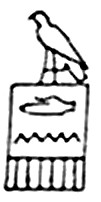
\includegraphics{src/../images/hand.jpg} &

\includegraphics{src/../images/mayan-glyph.png} \\
\end{longtable}

\subsection*{Data Glyph}\label{data-glyph}
\addcontentsline{toc}{subsection}{Data Glyph}

A data glyph is also a mark, e.g.


\includegraphics{src/../images/geom_rect.png}

\includegraphics{src/../images/geom_segment.png}
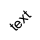
\includegraphics{src/../images/geom_text.png}

\includegraphics{src/../images/geom_crossbar.png}

\includegraphics{src/../images/geom_path.png}
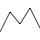
\includegraphics{src/../images/geom_line.png}
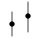
\includegraphics{src/../images/geom_pointrange.png}

\includegraphics{src/../images/geom_ribbon.png}

\includegraphics{src/../images/geom_point.png}

\includegraphics{src/../images/geom_polygon.png}

\includegraphics{src/../images/geom_histogram.png}

\includegraphics{src/../images/geom_dotplot.png}
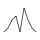
\includegraphics{src/../images/geom_freqpoly.png}
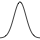
\includegraphics{src/../images/geom_density.png}

\includegraphics{src/../images/geom_violin.png}

The features of a data glyph encodes the value of variables.

\begin{itemize}
\tightlist
\item
  Some are very simple, e.g.~a dot:
  
\includegraphics{src/../images/geom_point.png}
\item
  Some combine different elements, e.g.~a pointrange:
  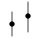
\includegraphics{src/../images/geom_pointrange.png}
\item
  Some are complicated, e.g.~a dotplot:
  
\includegraphics{src/../images/geom_dotplot.png}
\end{itemize}

\subsection*{Components of Graphics}\label{components-of-graphics}
\addcontentsline{toc}{subsection}{Components of Graphics}

\begin{figure}

\centering{

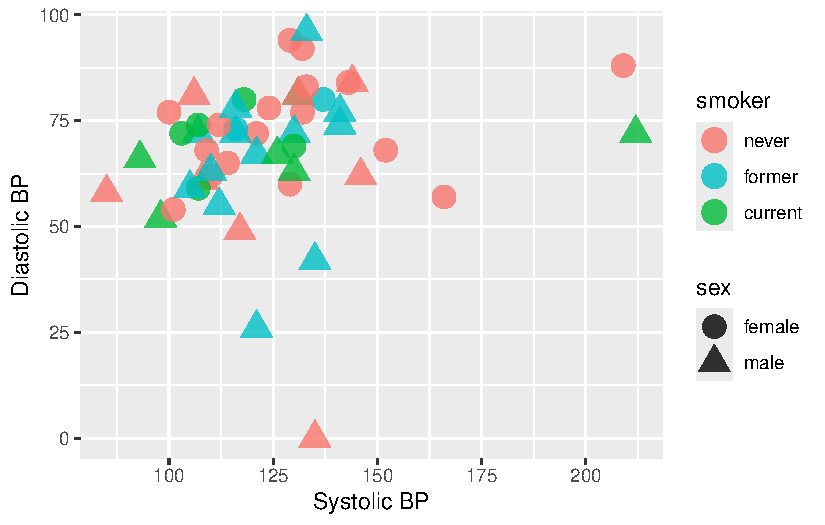
\includegraphics{src/02-Intro_Data_Viz_files/figure-pdf/fig-bp-1.pdf}

}

\caption{\label{fig-bp}Blood pressure readings from a random subset of
the NHANES data set.}

\end{figure}%

\begin{itemize}
\item
  \textbf{frame}: The position scale describing how data are mapped to x
  and y
\item
  \textbf{glyph}: The basic graphical unit that represents one case.

  \begin{itemize}
  \tightlist
  \item
    other terms used include \emph{mark} and \emph{symbol}.
  \end{itemize}
\item
  \textbf{aesthetic}: a visual property of a glyph such as position,
  size, shape, color, etc.

  \begin{itemize}
  \tightlist
  \item
    may be \textbf{mapped} based on data values:
    \texttt{smoker\ -\textgreater{}\ color}
  \item
    may be \textbf{set} to particular non-data related values:
    \texttt{color\ is\ black}
  \end{itemize}
\item
  \textbf{facet}: a subplot that shows one subset of the data

  \begin{itemize}
  \tightlist
  \item
    rather than represent \texttt{sex} by shape, we could split into two
    subplots
  \end{itemize}
\item
  \textbf{scale}: A mapping that translates data values into aesthetics.

  \begin{itemize}
  \tightlist
  \item
    example: never-\textgreater{} pink; former-\textgreater{} aqua;
    current-\textgreater{} green
  \end{itemize}
\item
  \textbf{guide}: An indication for the human viewer of the scale. This
  allows the viewer to translate aesthetics back into data values.

  \begin{itemize}
  \tightlist
  \item
    examples: x- and y-axes, various sorts of legends
  \end{itemize}
\end{itemize}

\subsection*{Eye Training for the Layered Grammar of
Graphics}\label{eye-training-for-the-layered-grammar-of-graphics}
\addcontentsline{toc}{subsection}{Eye Training for the Layered Grammar
of Graphics}

\begin{Shaded}
\begin{Highlighting}[]
\NormalTok{For your assigned graphic, discuss the following seven questions with your partner(s):}

\NormalTok{1. What variables constitute the frame?}
\NormalTok{2. What glyphs are used?}
\NormalTok{3. What are the aesthetics for those glyphs?}
\NormalTok{4. Which variable is mapped to each aesthetic?}
\NormalTok{5. Which variable, if any, is used for faceting?}
\NormalTok{6. Which scales are displayed with a guide?}
\NormalTok{7. What raw data would be required for this plot, and what form should it be in?}

\NormalTok{Here are the graphics examples, all taken from the New York Times website:}

\NormalTok{a. [Admissions gap](http://www.nytimes.com/interactive/2013/05/07/education/college{-}admissions{-}gap.html?\_r=0)}
\NormalTok{\#. [Medicare hospital charges](https://www.nytimes.com/interactive/2014/06/02/business/how{-}much{-}hospitals{-}charged{-}medicare{-}for{-}the{-}same{-}procedures.html)}
\NormalTok{\#. [Football conferences](http://www.nytimes.com/newsgraphics/2013/11/30/football{-}conferences/)}
\NormalTok{\#. [Housing prices](https://www.nytimes.com/interactive/2014/01/23/business/case{-}shiller{-}slider.html)}
\NormalTok{\#. [Baseball pitching](http://www.nytimes.com/interactive/2013/03/29/sports/baseball/Strikeouts{-}Are{-}Still{-}Soaring.html)}
\NormalTok{\#. [Phillips curve](http://www.nytimes.com/interactive/2013/10/09/us/yellen{-}fed{-}chart.html)}
\NormalTok{\#. [School mathematics ratings](http://www.nytimes.com/interactive/2013/02/04/science/girls{-}lead{-}in{-}science{-}exam{-}but{-}not{-}in{-}the{-}united{-}states.html)}
\NormalTok{\#. [Corporate taxes](http://www.nytimes.com/interactive/2013/05/25/sunday{-}review/corporate{-}taxes.html)}
\end{Highlighting}
\end{Shaded}

\subsection*{Glyph-Ready Data}\label{glyph-ready-data}
\addcontentsline{toc}{subsection}{Glyph-Ready Data}

Note the mapping of data to aesthetics for Figure @ref(fig:fig-bp):

\begin{verbatim}
   sbp [Systolic Blood Pressure] -> x      
   dbp [Diastolic Blood Pressure] -> y     
smoker -> color
   sex -> shape
\end{verbatim}

Glyph-ready data has this form:

\begin{itemize}
\tightlist
\item
  There is one row for each glyph to be drawn.
\item
  The variables in that row are mapped to aesthetics of the glyph
  (including position).
\end{itemize}

\begin{longtable}[]{@{}rrll@{}}
\caption{A subset of the NHANES data set.}\tabularnewline
\toprule\noalign{}
sbp & dbp & sex & smoker \\
\midrule\noalign{}
\endfirsthead
\toprule\noalign{}
sbp & dbp & sex & smoker \\
\midrule\noalign{}
\endhead
\bottomrule\noalign{}
\endlastfoot
112 & 55 & male & former \\
144 & 84 & male & never \\
143 & 84 & female & never \\
110 & 62 & female & never \\
121 & 72 & female & never \\
129 & 60 & female & never \\
\end{longtable}

\section*{\texorpdfstring{Data Visualization Workflow +
\texttt{ggplot}}{Data Visualization Workflow + ggplot}}\label{data-visualization-workflow-ggplot}
\addcontentsline{toc}{section}{Data Visualization Workflow +
\texttt{ggplot}}

\markright{Data Visualization Workflow + \texttt{ggplot}}

\subsection*{Layers -- Building up Complex
Plots}\label{layers-building-up-complex-plots}
\addcontentsline{toc}{subsection}{Layers -- Building up Complex Plots}

Using the \texttt{ggplot2} package, we can create graphics by building
up layers, each of which may have its own data, glyphs, aesthetic
mapping, etc. As an example, let's peel back the layers used to create
Figure @ref(fig:fig-bp).

The first layer just identifies the data set. It sets up a blank canvas,
but does not actually plot anything:

\begin{Shaded}
\begin{Highlighting}[]
\FunctionTok{ggplot}\NormalTok{(}\AttributeTok{data =}\NormalTok{ Tmp)}
\end{Highlighting}
\end{Shaded}


\includegraphics{src/02-Intro_Data_Viz_files/figure-pdf/unnamed-chunk-4-1.pdf}

Next, we add a geometry layer to identify the mapping of data to
aesthetics for each of the glyphs:

\begin{Shaded}
\begin{Highlighting}[]
\FunctionTok{ggplot}\NormalTok{(}\AttributeTok{data =}\NormalTok{ Tmp) }\SpecialCharTok{+}
  \FunctionTok{geom\_point}\NormalTok{(}\AttributeTok{mapping =} \FunctionTok{aes}\NormalTok{(}\AttributeTok{x =}\NormalTok{ sbp, }\AttributeTok{y =}\NormalTok{ dbp, }\AttributeTok{shape =}\NormalTok{ sex, }\AttributeTok{color =}\NormalTok{ smoker), }\AttributeTok{size =} \DecValTok{5}\NormalTok{, }\AttributeTok{alpha =}\NormalTok{ .}\DecValTok{8}\NormalTok{)}
\end{Highlighting}
\end{Shaded}

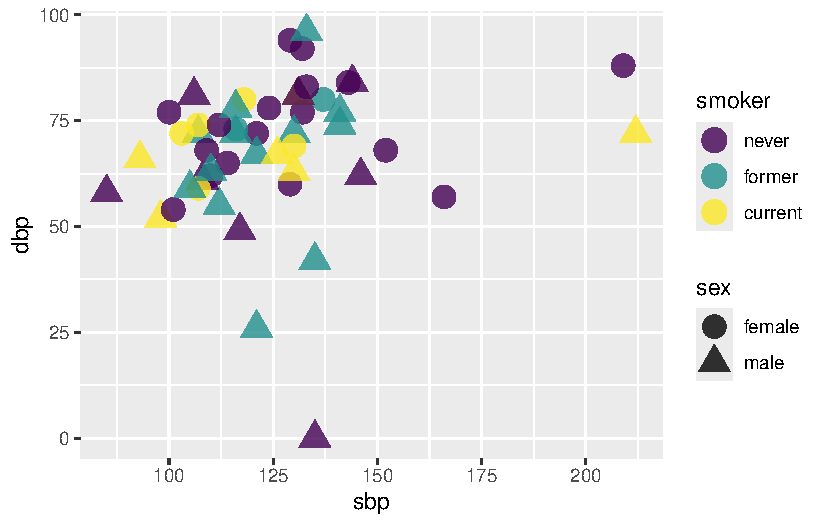
\includegraphics{src/02-Intro_Data_Viz_files/figure-pdf/unnamed-chunk-5-1.pdf}

Next, we can add some axes labels as guides:

\begin{Shaded}
\begin{Highlighting}[]
\FunctionTok{ggplot}\NormalTok{(}\AttributeTok{data =}\NormalTok{ Tmp) }\SpecialCharTok{+}
  \FunctionTok{geom\_point}\NormalTok{(}\AttributeTok{mapping =} \FunctionTok{aes}\NormalTok{(}\AttributeTok{x =}\NormalTok{ sbp, }\AttributeTok{y =}\NormalTok{ dbp, }\AttributeTok{shape =}\NormalTok{ sex, }\AttributeTok{color =}\NormalTok{ smoker), }\AttributeTok{size =} \DecValTok{5}\NormalTok{, }\AttributeTok{alpha =}\NormalTok{ .}\DecValTok{8}\NormalTok{) }\SpecialCharTok{+}
  \FunctionTok{xlab}\NormalTok{(}\StringTok{"Systolic BP"}\NormalTok{) }\SpecialCharTok{+} \FunctionTok{ylab}\NormalTok{(}\StringTok{"Diastolic BP"}\NormalTok{)}
\end{Highlighting}
\end{Shaded}

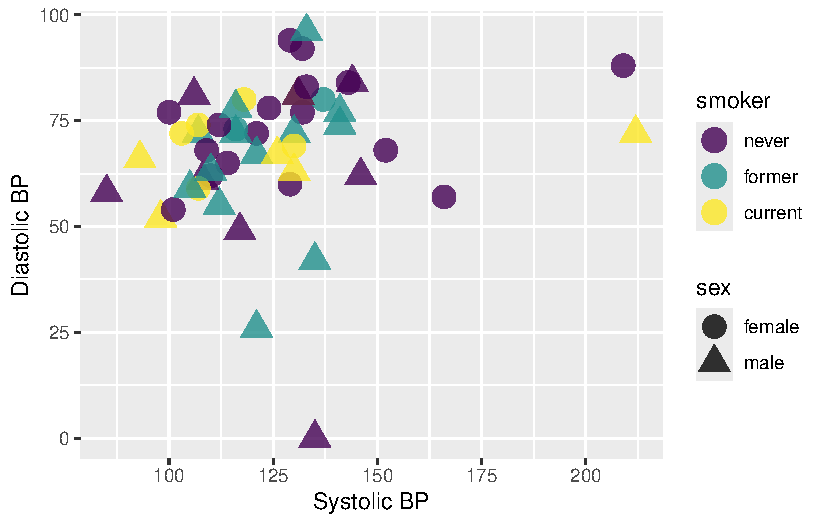
\includegraphics{src/02-Intro_Data_Viz_files/figure-pdf/unnamed-chunk-6-1.pdf}

And, finally, we can change the scale of the color used for smoker
status:

\begin{Shaded}
\begin{Highlighting}[]
\FunctionTok{ggplot}\NormalTok{(}\AttributeTok{data =}\NormalTok{ Tmp) }\SpecialCharTok{+}
  \FunctionTok{geom\_point}\NormalTok{(}\AttributeTok{mapping =} \FunctionTok{aes}\NormalTok{(}\AttributeTok{x =}\NormalTok{ sbp, }\AttributeTok{y =}\NormalTok{ dbp, }\AttributeTok{shape =}\NormalTok{ sex, }\AttributeTok{color =}\NormalTok{ smoker), }\AttributeTok{size =} \DecValTok{5}\NormalTok{, }\AttributeTok{alpha =}\NormalTok{ .}\DecValTok{8}\NormalTok{) }\SpecialCharTok{+}
  \FunctionTok{xlab}\NormalTok{(}\StringTok{"Systolic BP"}\NormalTok{) }\SpecialCharTok{+} \FunctionTok{ylab}\NormalTok{(}\StringTok{"Diastolic BP"}\NormalTok{) }\SpecialCharTok{+}
  \FunctionTok{scale\_color\_manual}\NormalTok{(}\AttributeTok{values =} \FunctionTok{c}\NormalTok{(}\StringTok{"\#F8766D"}\NormalTok{, }\StringTok{"\#00BFC4"}\NormalTok{, }\StringTok{"\#00BA38"}\NormalTok{))}
\end{Highlighting}
\end{Shaded}

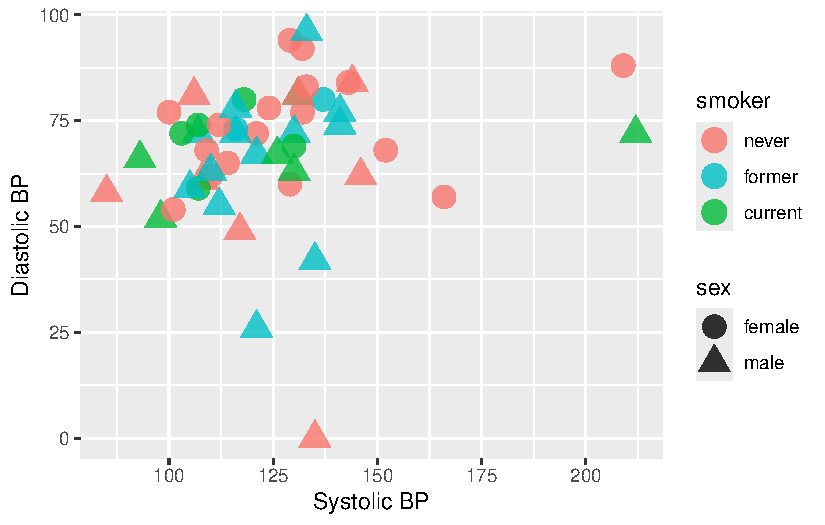
\includegraphics{src/02-Intro_Data_Viz_files/figure-pdf/unnamed-chunk-7-1.pdf}

If instead we wanted to facet into columns based on smoker status, we
could add another layer for that:

\begin{Shaded}
\begin{Highlighting}[]
\FunctionTok{ggplot}\NormalTok{(}\AttributeTok{data =}\NormalTok{ Tmp) }\SpecialCharTok{+}
  \FunctionTok{geom\_point}\NormalTok{(}\AttributeTok{mapping =} \FunctionTok{aes}\NormalTok{(}\AttributeTok{x =}\NormalTok{ sbp, }\AttributeTok{y =}\NormalTok{ dbp, }\AttributeTok{shape =}\NormalTok{ sex, }\AttributeTok{color =}\NormalTok{ smoker), }\AttributeTok{size =} \DecValTok{5}\NormalTok{, }\AttributeTok{alpha =}\NormalTok{ .}\DecValTok{8}\NormalTok{) }\SpecialCharTok{+}
  \FunctionTok{xlab}\NormalTok{(}\StringTok{"Systolic BP"}\NormalTok{) }\SpecialCharTok{+} \FunctionTok{ylab}\NormalTok{(}\StringTok{"Diastolic BP"}\NormalTok{) }\SpecialCharTok{+}
  \FunctionTok{scale\_color\_manual}\NormalTok{(}\AttributeTok{values =} \FunctionTok{c}\NormalTok{(}\StringTok{"\#F8766D"}\NormalTok{, }\StringTok{"\#00BFC4"}\NormalTok{, }\StringTok{"\#00BA38"}\NormalTok{)) }\SpecialCharTok{+}
  \FunctionTok{facet\_grid}\NormalTok{(. }\SpecialCharTok{\textasciitilde{}}\NormalTok{ smoker)}
\end{Highlighting}
\end{Shaded}

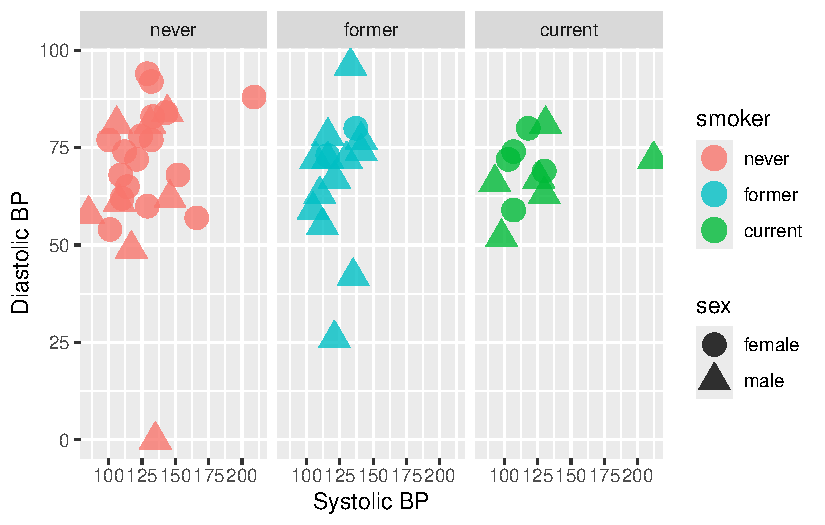
\includegraphics{src/02-Intro_Data_Viz_files/figure-pdf/unnamed-chunk-8-1.pdf}

For more information on all of the different types of layers we can add
to graphics, see the
\href{https://ggplot2.tidyverse.org/reference/}{\texttt{ggplot2}
reference page} and the
\href{https://raw.githubusercontent.com/rstudio/cheatsheets/main/data-visualization.pdf}{data
visualization with \texttt{ggplot2} cheat sheet}.

\subsection*{Getting Started}\label{getting-started}
\addcontentsline{toc}{subsection}{Getting Started}

There's no end to the number and type of visualizations you \emph{could}
make. Thus the process can feel overwhelming.
\href{http://flowingdata.com/2017/01/24/one-dataset-visualized-25-ways/}{FlowingData}
makes good recommendations for data viz workflow:

\begin{itemize}
\tightlist
\item
  \textbf{Ask the data questions.} Simple research questions will guide
  the types of visualizations that you should construct.\\
\item
  \textbf{Start with the basics and work incrementally.} Before
  constructing complicated or multivariate or interactive graphics,
  start with simple visualizations. An understanding of the simple
  patterns provides a foundation upon which to build more advanced
  analyses and visualizations. This incremental process works
  particularly well with the layered grammar of graphics in
  \texttt{ggplot}.
\item
  \textbf{Focus.} Reporting a large number of visualizations can
  overwhelm the audience and obscure your conclusions. Instead, pick out
  a focused yet comprehensive set of visualizations.
  \href{http://flowingdata.com/2017/01/24/one-dataset-visualized-25-ways/}{Here}
  is an example of one dataset visualized 25 different ways, each with a
  different focus and interpretation, and what can happen if you let the
  data ramble on without a focus.
\end{itemize}

In this course we'll largely construct visualizations using the
\texttt{ggplot} function in RStudio. Though the \texttt{ggplot} learning
curve can be steep, its ``grammar'' is intuitive and generalizable once
mastered. The \texttt{ggplot} plotting function is stored in the
\texttt{ggplot2} package:

\begin{Shaded}
\begin{Highlighting}[]
\FunctionTok{library}\NormalTok{(ggplot2)}
\end{Highlighting}
\end{Shaded}

The best way to learn about \texttt{ggplot} is to just play around.
Focus on the \emph{patterns} and \emph{potential} of their application.
It will be helpful to have the
\href{https://raw.githubusercontent.com/rstudio/cheatsheets/main/data-visualization.pdf}{RStudio
Data Visualization cheat sheet} handy as you complete this activity.

\subsection*{An Example}\label{an-example}
\addcontentsline{toc}{subsection}{An Example}

The ``Bechdel test'', named after cartoonist Alison Bechdel, tests
whether movies meet the following criteria:

\begin{enumerate}
\def\labelenumi{\arabic{enumi}.}
\tightlist
\item
  There are \(\ge\) 2 (named) female characters;\\
\item
  these women talk to each other\ldots{}\\
\item
  about something other than a man.
\end{enumerate}

In the fivethirtyeight.com article
\href{http://fivethirtyeight.com/features/the-dollar-and-cents-case-against-hollywoods-exclusion-of-women/}{``The
Dollar-And-Cents Case Against Hollywood's Exclusion of Women''}, the
authors analyze which Hollywood movies do/don't pass the test. Their
data are available in the \texttt{fivethirtyeight} package:

\begin{Shaded}
\begin{Highlighting}[]
\FunctionTok{library}\NormalTok{(fivethirtyeight)}
\FunctionTok{data}\NormalTok{(bechdel)}
\FunctionTok{head}\NormalTok{(bechdel)}
\end{Highlighting}
\end{Shaded}

\begin{longtable}[]{@{}
  >{\raggedleft\arraybackslash}p{(\columnwidth - 14\tabcolsep) * \real{0.0556}}
  >{\raggedright\arraybackslash}p{(\columnwidth - 14\tabcolsep) * \real{0.1111}}
  >{\raggedright\arraybackslash}p{(\columnwidth - 14\tabcolsep) * \real{0.1889}}
  >{\raggedright\arraybackslash}p{(\columnwidth - 14\tabcolsep) * \real{0.1222}}
  >{\raggedright\arraybackslash}p{(\columnwidth - 14\tabcolsep) * \real{0.0778}}
  >{\raggedleft\arraybackslash}p{(\columnwidth - 14\tabcolsep) * \real{0.1333}}
  >{\raggedleft\arraybackslash}p{(\columnwidth - 14\tabcolsep) * \real{0.1556}}
  >{\raggedleft\arraybackslash}p{(\columnwidth - 14\tabcolsep) * \real{0.1556}}@{}}
\toprule\noalign{}
\begin{minipage}[b]{\linewidth}\raggedleft
year
\end{minipage} & \begin{minipage}[b]{\linewidth}\raggedright
imdb
\end{minipage} & \begin{minipage}[b]{\linewidth}\raggedright
title
\end{minipage} & \begin{minipage}[b]{\linewidth}\raggedright
clean\_test
\end{minipage} & \begin{minipage}[b]{\linewidth}\raggedright
binary
\end{minipage} & \begin{minipage}[b]{\linewidth}\raggedleft
budget\_2013
\end{minipage} & \begin{minipage}[b]{\linewidth}\raggedleft
domgross\_2013
\end{minipage} & \begin{minipage}[b]{\linewidth}\raggedleft
intgross\_2013
\end{minipage} \\
\midrule\noalign{}
\endhead
\bottomrule\noalign{}
\endlastfoot
2013 & tt1711425 & 21 \& Over & notalk & FAIL & 13000000 & 25682380 &
42195766 \\
2012 & tt1343727 & Dredd 3D & ok & PASS & 45658735 & 13611086 &
41467257 \\
2013 & tt2024544 & 12 Years a Slave & notalk & FAIL & 20000000 &
53107035 & 158607035 \\
2013 & tt1272878 & 2 Guns & notalk & FAIL & 61000000 & 75612460 &
132493015 \\
2013 & tt0453562 & 42 & men & FAIL & 40000000 & 95020213 & 95020213 \\
2013 & tt1335975 & 47 Ronin & men & FAIL & 225000000 & 38362475 &
145803842 \\
\end{longtable}

\begin{Shaded}
\begin{Highlighting}[]
\NormalTok{Before diving into any visualizations of these data, we first must understand its structure and contents. Discuss the following:  }
  
\NormalTok{  a. What are the units of observation and how many units are in this sample? }
\NormalTok{  b. What are the levels of the \textasciigrave{}clean\_test\textasciigrave{} and \textasciigrave{}binary\textasciigrave{} categorical variables?    }
\NormalTok{  c. Check out the codebook for \textasciigrave{}bechdel\textasciigrave{} (\textasciigrave{}?bechdel\textasciigrave{}).  What\textquotesingle{}s the difference between \textasciigrave{}domgross\_2013\textasciigrave{} and \textasciigrave{}domgross\textasciigrave{}?    }
\end{Highlighting}
\end{Shaded}

Solution

\begin{Shaded}
\begin{Highlighting}[]
\CommentTok{\#units of observation are movies; there are 1794 movies in this sample}
\FunctionTok{dim}\NormalTok{(bechdel)}
\DocumentationTok{\#\# [1] 1794   15}

\CommentTok{\#clean\_test has values of "nowomen", "notalk", "men", "dubious", "ok"}
\CommentTok{\#View(bchedel) and look at values or summarize like below}
\FunctionTok{table}\NormalTok{(bechdel}\SpecialCharTok{$}\NormalTok{clean\_test)}
\DocumentationTok{\#\# }
\DocumentationTok{\#\# nowomen  notalk     men dubious      ok }
\DocumentationTok{\#\#     141     514     194     142     803}
\FunctionTok{levels}\NormalTok{(bechdel}\SpecialCharTok{$}\NormalTok{clean\_test)}
\DocumentationTok{\#\# [1] "nowomen" "notalk"  "men"     "dubious" "ok"}

\CommentTok{\#binary has values of PASS or FAIL}
\FunctionTok{table}\NormalTok{(bechdel}\SpecialCharTok{$}\NormalTok{binary)}
\DocumentationTok{\#\# }
\DocumentationTok{\#\# FAIL PASS }
\DocumentationTok{\#\#  991  803}
\FunctionTok{levels}\NormalTok{(}\FunctionTok{factor}\NormalTok{(bechdel}\SpecialCharTok{$}\NormalTok{binary))}
\DocumentationTok{\#\# [1] "FAIL" "PASS"}

\CommentTok{\# domgross\_2013 is the domestic gross in US dollars but it is inflation adjusted with respect to 2013}
\CommentTok{\#?bechdel}
\end{Highlighting}
\end{Shaded}

\hfill\break

\begin{Shaded}
\begin{Highlighting}[]
\NormalTok{We\textquotesingle{}ll consider *univariate* visualizations of the \textasciigrave{}clean\_test\textasciigrave{} and \textasciigrave{}budget\_2013\textasciigrave{} variables. Discuss the following:}
  
\NormalTok{  a. What features would we like a visualization of the *categorical* \textasciigrave{}clean\_test\textasciigrave{} variable to capture?    }
\NormalTok{  b. What features would we like a visualization of the *quantitative* \textasciigrave{}budget\_2013\textasciigrave{} variable to capture?    }
\end{Highlighting}
\end{Shaded}

Solution

\begin{enumerate}
\def\labelenumi{\alph{enumi}.}
\tightlist
\item
  capture the frequency of each way a movie can fail or pass the Bechdel
  test
\item
  capture the typical budget as well as how much variation there is
  across movies and if there are any outliers
\end{enumerate}

\hfill\break

\subsection*{Categorical univariate
visualization}\label{categorical-univariate-visualization}
\addcontentsline{toc}{subsection}{Categorical univariate visualization}

We begin by stating a clear research question:

\begin{quote}
Among the movies in our sample, what fraction pass the Bechdel test?
Among those that fail the test, in which way do they fail (e.g., there
are no women, there are women but they only talk about men,\ldots)?
\end{quote}

To answer the above research question, we can explore the categorical
\texttt{clean\_test} variable. A table provides a simple summary of the
number of movies that fall into each \texttt{clean\_test} category:

\begin{Shaded}
\begin{Highlighting}[]
\FunctionTok{table}\NormalTok{(bechdel}\SpecialCharTok{$}\NormalTok{clean\_test)}
\end{Highlighting}
\end{Shaded}

\begin{verbatim}

nowomen  notalk     men dubious      ok 
    141     514     194     142     803 
\end{verbatim}

\begin{Shaded}
\begin{Highlighting}[]
\NormalTok{Examine the table of \textasciigrave{}clean\_test\textasciigrave{} data, and try to interpret it. What insights does it provide about the original research question?}
\end{Highlighting}
\end{Shaded}

Solution

Among the categories, the ``ok'' category was most frequent, meaning
that 803 of the 1794 movies in the sample passed the Bechdel Test.
However, among those 991 movies that did not pass the test, most of them
(514 of them) did not pass because the women did not talk.

\hfill\break

Because \texttt{clean\_test} is a categorical variable, a \textbf{bar
chart} provides an appropriate visualization of this table. In examining
the bar chart, keep your eyes on the following.

\begin{itemize}
\tightlist
\item
  \textbf{variability}: Are cases evenly spread out among the categories
  or are some categories more common than others?\\
\item
  \textbf{contextual implications}: In the context of your research,
  what do you learn from the bar chart? How would you describe your
  findings to a broad audience?
\end{itemize}

\begin{Shaded}
\begin{Highlighting}[]
\NormalTok{Try out the code below that builds up from a simple to a customized bar chart. At each step determine how each piece of code contributes to the plot and add a comment describe the addition.    }
\end{Highlighting}
\end{Shaded}

\begin{Shaded}
\begin{Highlighting}[]
\CommentTok{\# plot 1: set up a plotting frame (a blank canvas)}
\FunctionTok{ggplot}\NormalTok{(bechdel, }\FunctionTok{aes}\NormalTok{(}\AttributeTok{x =}\NormalTok{ clean\_test))}

\CommentTok{\# plot 2: what changed / how did we change it?}
\FunctionTok{ggplot}\NormalTok{(bechdel, }\FunctionTok{aes}\NormalTok{(}\AttributeTok{x =}\NormalTok{ clean\_test)) }\SpecialCharTok{+}
\FunctionTok{geom\_bar}\NormalTok{()}

\CommentTok{\# plot 3: what changed / how did we change it?}
\FunctionTok{ggplot}\NormalTok{(bechdel, }\FunctionTok{aes}\NormalTok{(}\AttributeTok{x =}\NormalTok{ clean\_test)) }\SpecialCharTok{+}
\FunctionTok{geom\_bar}\NormalTok{() }\SpecialCharTok{+}
\FunctionTok{labs}\NormalTok{(}\AttributeTok{x =} \StringTok{"Outcome of Bechdel Test"}\NormalTok{, }\AttributeTok{y =} \StringTok{"Number of movies"}\NormalTok{)}

\CommentTok{\# plot 4: what changed / how did we change it?}
\FunctionTok{ggplot}\NormalTok{(bechdel, }\FunctionTok{aes}\NormalTok{(}\AttributeTok{x =}\NormalTok{ clean\_test)) }\SpecialCharTok{+}
\FunctionTok{geom\_bar}\NormalTok{(}\AttributeTok{color =} \StringTok{"purple"}\NormalTok{) }\SpecialCharTok{+}
\FunctionTok{labs}\NormalTok{(}\AttributeTok{x =} \StringTok{"Outcome of Bechdel Test"}\NormalTok{, }\AttributeTok{y =} \StringTok{"Number of movies"}\NormalTok{)}

\CommentTok{\# plot 5: what changed / how did we change it?}
\FunctionTok{ggplot}\NormalTok{(bechdel, }\FunctionTok{aes}\NormalTok{(}\AttributeTok{x =}\NormalTok{ clean\_test)) }\SpecialCharTok{+}
\FunctionTok{geom\_bar}\NormalTok{(}\AttributeTok{fill =} \StringTok{"purple"}\NormalTok{) }\SpecialCharTok{+}
\FunctionTok{labs}\NormalTok{(}\AttributeTok{x =} \StringTok{"Outcome of Bechdel Test"}\NormalTok{, }\AttributeTok{y =} \StringTok{"Number of movies"}\NormalTok{)}
\end{Highlighting}
\end{Shaded}

Solution

\begin{Shaded}
\begin{Highlighting}[]
\CommentTok{\# plot 1: set up a plotting frame (a blank canvas)}
\FunctionTok{ggplot}\NormalTok{(bechdel, }\FunctionTok{aes}\NormalTok{(}\AttributeTok{x =}\NormalTok{ clean\_test))}
\end{Highlighting}
\end{Shaded}

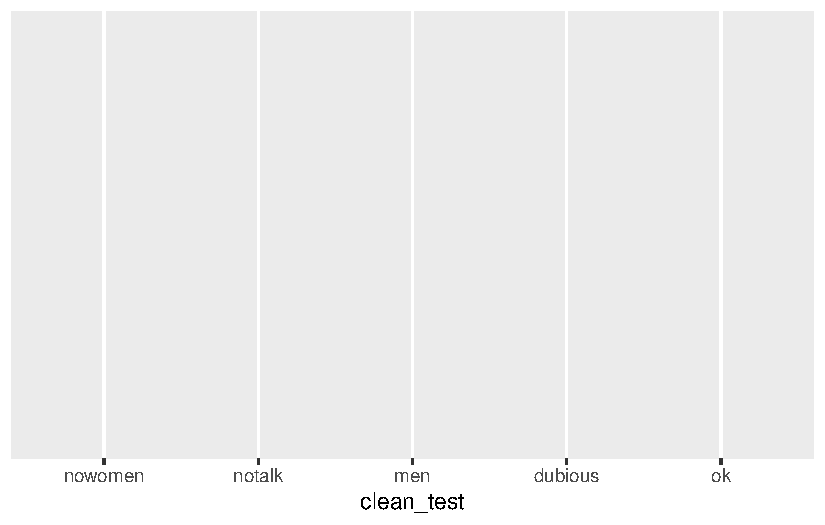
\includegraphics{src/02-Intro_Data_Viz_files/figure-pdf/unnamed-chunk-19-1.pdf}

\begin{Shaded}
\begin{Highlighting}[]

\CommentTok{\# plot 2: Added bars that reflect the count or frequency of the movies within each category}
\FunctionTok{ggplot}\NormalTok{(bechdel, }\FunctionTok{aes}\NormalTok{(}\AttributeTok{x =}\NormalTok{ clean\_test)) }\SpecialCharTok{+}
\FunctionTok{geom\_bar}\NormalTok{()}
\end{Highlighting}
\end{Shaded}

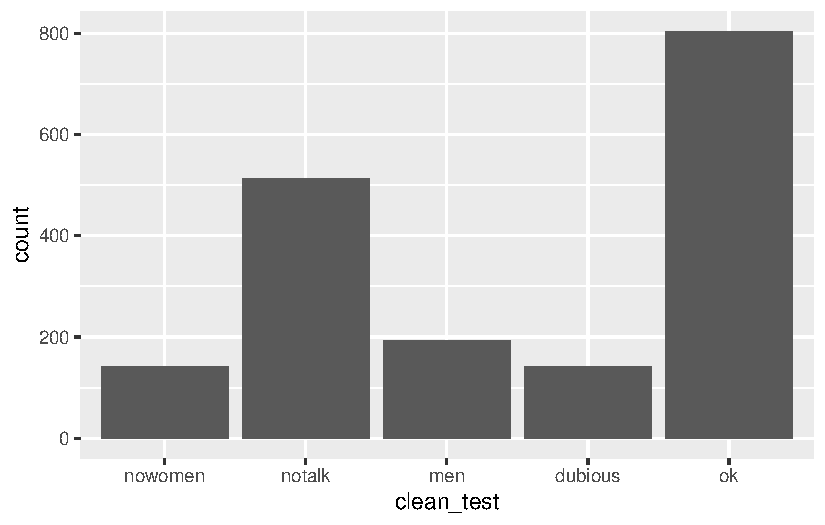
\includegraphics{src/02-Intro_Data_Viz_files/figure-pdf/unnamed-chunk-19-2.pdf}

\begin{Shaded}
\begin{Highlighting}[]

\CommentTok{\# plot 3: Added/changed the text labels for the x and y axes}
\FunctionTok{ggplot}\NormalTok{(bechdel, }\FunctionTok{aes}\NormalTok{(}\AttributeTok{x =}\NormalTok{ clean\_test)) }\SpecialCharTok{+}
\FunctionTok{geom\_bar}\NormalTok{() }\SpecialCharTok{+}
\FunctionTok{labs}\NormalTok{(}\AttributeTok{x =} \StringTok{"Outcome of Bechdel Test"}\NormalTok{, }\AttributeTok{y =} \StringTok{"Number of movies"}\NormalTok{)}
\end{Highlighting}
\end{Shaded}

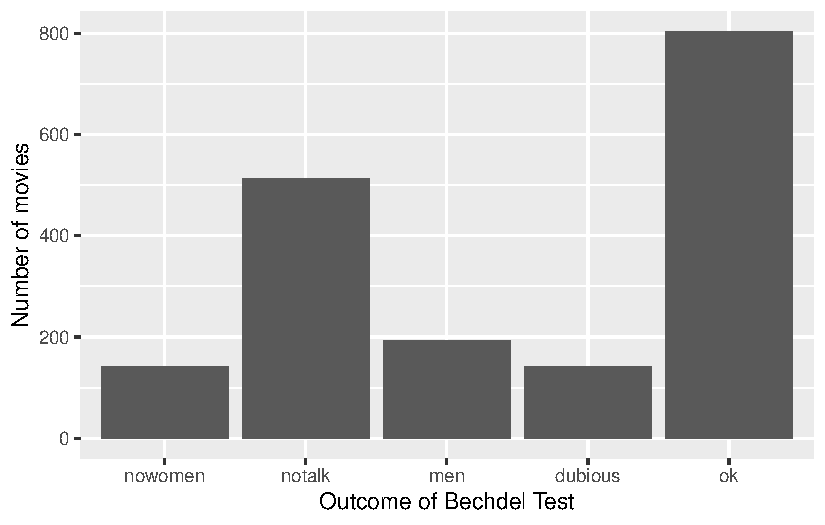
\includegraphics{src/02-Intro_Data_Viz_files/figure-pdf/unnamed-chunk-19-3.pdf}

\begin{Shaded}
\begin{Highlighting}[]

\CommentTok{\# plot 4: Changed the outline color of the bars to purple}
\FunctionTok{ggplot}\NormalTok{(bechdel, }\FunctionTok{aes}\NormalTok{(}\AttributeTok{x =}\NormalTok{ clean\_test)) }\SpecialCharTok{+}
\FunctionTok{geom\_bar}\NormalTok{(}\AttributeTok{color =} \StringTok{"purple"}\NormalTok{) }\SpecialCharTok{+}
\FunctionTok{labs}\NormalTok{(}\AttributeTok{x =} \StringTok{"Outcome of Bechdel Test"}\NormalTok{, }\AttributeTok{y =} \StringTok{"Number of movies"}\NormalTok{)}
\end{Highlighting}
\end{Shaded}

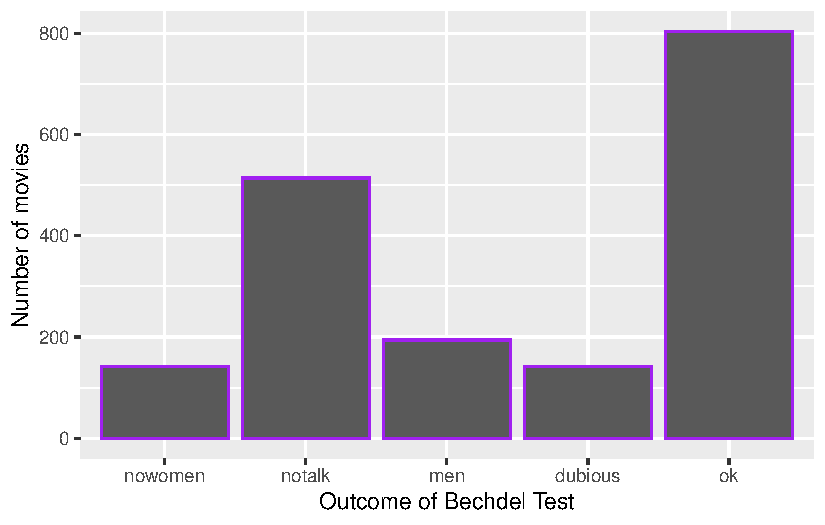
\includegraphics{src/02-Intro_Data_Viz_files/figure-pdf/unnamed-chunk-19-4.pdf}

\begin{Shaded}
\begin{Highlighting}[]

\CommentTok{\# plot 5: Changed the fill  color of the bars to purple}
\FunctionTok{ggplot}\NormalTok{(bechdel, }\FunctionTok{aes}\NormalTok{(}\AttributeTok{x =}\NormalTok{ clean\_test)) }\SpecialCharTok{+}
\FunctionTok{geom\_bar}\NormalTok{(}\AttributeTok{fill =} \StringTok{"purple"}\NormalTok{) }\SpecialCharTok{+}
\FunctionTok{labs}\NormalTok{(}\AttributeTok{x =} \StringTok{"Outcome of Bechdel Test"}\NormalTok{, }\AttributeTok{y =} \StringTok{"Number of movies"}\NormalTok{)}
\end{Highlighting}
\end{Shaded}

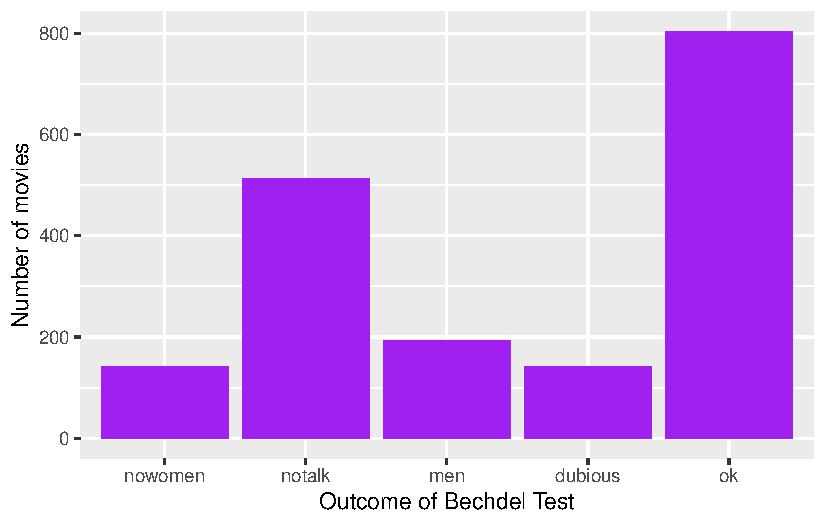
\includegraphics{src/02-Intro_Data_Viz_files/figure-pdf/unnamed-chunk-19-5.pdf}

\hfill\break

\begin{Shaded}
\begin{Highlighting}[]
\NormalTok{Summarize the visualization: what did you learn about the distribution of the \textasciigrave{}clean\_test\textasciigrave{} variable?    }
\end{Highlighting}
\end{Shaded}

Solution

Among the categories, the ``ok'' category was most frequent. However,
among those movies that did not pass the test, most of them did not pass
because the women in the movie did not talk.

\hfill\break

\begin{Shaded}
\begin{Highlighting}[]
\NormalTok{Let\textquotesingle{}s return to our research question: What percent of movies in the sample pass the Bechdel test? Among those that fail the test, in which way do they fail? }
\end{Highlighting}
\end{Shaded}

Solution

\begin{Shaded}
\begin{Highlighting}[]
\FunctionTok{table}\NormalTok{(bechdel}\SpecialCharTok{$}\NormalTok{binary)}
\DocumentationTok{\#\# }
\DocumentationTok{\#\# FAIL PASS }
\DocumentationTok{\#\#  991  803}
\DecValTok{803}\SpecialCharTok{/}\NormalTok{(}\DecValTok{991} \SpecialCharTok{+} \DecValTok{803}\NormalTok{)}
\DocumentationTok{\#\# [1] 0.4476031}


\FunctionTok{table}\NormalTok{(bechdel}\SpecialCharTok{$}\NormalTok{clean\_test)[}\DecValTok{1}\SpecialCharTok{:}\DecValTok{4}\NormalTok{]}\SpecialCharTok{/}\DecValTok{991}
\DocumentationTok{\#\# }
\DocumentationTok{\#\#   nowomen    notalk       men   dubious }
\DocumentationTok{\#\# 0.1422805 0.5186680 0.1957619 0.1432896}
\end{Highlighting}
\end{Shaded}

\hfill\break

\subsection*{Quantitative univariate
visualization}\label{quantitative-univariate-visualization}
\addcontentsline{toc}{subsection}{Quantitative univariate visualization}

To motivate quantitative visualizations, consider a second research
question

\begin{quote}
Among the movies in our sample, what's the range of budgets? What's the
typical budget? The largest/smallest?
\end{quote}

We can answer the above research question by exploring the
\emph{quantitative} \texttt{budget\_2013} variable. Quantitative
variables require different summary tools than categorical variables.
We'll explore two methods for graphing quantitative variables:
histograms and density plots. Both of these has strengths/weaknesses in
helping us visualize the distribution of observed values.

In their examination, keep your eyes on the following.

\begin{itemize}
\tightlist
\item
  \textbf{center}: Where's the center of the distribution? What's a
  typical value of the variable?
\item
  \textbf{variability}: How spread out are the values? A lot or a
  little?
\item
  \textbf{shape}: How are values distributed along the observed range?
  Is the distribution symmetric, right-skewed, left-skewed, bi-modal, or
  uniform (flat)?\\
\item
  \textbf{outliers}: Are there any \emph{outliers}, ie. values that are
  unusually large/small relative to the bulk of other values?\\
\item
  \textbf{contextual implications}: Interpret these features in the
  context of your research. How would you describe your findings to a
  broad audience?
\end{itemize}

\subsubsection*{Histograms}\label{histograms}
\addcontentsline{toc}{subsubsection}{Histograms}

Histograms are constructed by (1) dividing up the observed range of the
variable into `bins' of equal width; and (2) counting up the number of
cases that fall into each bin.

\begin{Shaded}
\begin{Highlighting}[]
\NormalTok{Try out the code below.  At each step determine how each piece of code contributes to the plot.    }
\end{Highlighting}
\end{Shaded}

\begin{Shaded}
\begin{Highlighting}[]
\CommentTok{\# plot 1: set up a plotting frame}
\FunctionTok{ggplot}\NormalTok{(bechdel, }\FunctionTok{aes}\NormalTok{(}\AttributeTok{x =}\NormalTok{ budget\_2013))}

\CommentTok{\# plot 2: what changed / how did we change it?}
\FunctionTok{ggplot}\NormalTok{(bechdel, }\FunctionTok{aes}\NormalTok{(}\AttributeTok{x =}\NormalTok{ budget\_2013)) }\SpecialCharTok{+}
  \FunctionTok{geom\_histogram}\NormalTok{()}

\CommentTok{\# plot 3: what changed / how did we change it?}
\FunctionTok{ggplot}\NormalTok{(bechdel, }\FunctionTok{aes}\NormalTok{(}\AttributeTok{x =}\NormalTok{ budget\_2013)) }\SpecialCharTok{+}
  \FunctionTok{geom\_histogram}\NormalTok{() }\SpecialCharTok{+}
  \FunctionTok{labs}\NormalTok{(}\AttributeTok{x =} \StringTok{"Budget ($)"}\NormalTok{, }\AttributeTok{y =} \StringTok{"Number of movies"}\NormalTok{)}

\CommentTok{\# plot 4: what changed / how did we change it?}
\FunctionTok{ggplot}\NormalTok{(bechdel, }\FunctionTok{aes}\NormalTok{(}\AttributeTok{x =}\NormalTok{ budget\_2013)) }\SpecialCharTok{+}
  \FunctionTok{geom\_histogram}\NormalTok{(}\AttributeTok{color =} \StringTok{"white"}\NormalTok{) }\SpecialCharTok{+}
  \FunctionTok{labs}\NormalTok{(}\AttributeTok{x =} \StringTok{"Budget ($)"}\NormalTok{, }\AttributeTok{y =} \StringTok{"Number of movies"}\NormalTok{)}

\CommentTok{\# plot 5: what changed / how did we change it?}
\FunctionTok{ggplot}\NormalTok{(bechdel, }\FunctionTok{aes}\NormalTok{(}\AttributeTok{x =}\NormalTok{ budget\_2013)) }\SpecialCharTok{+}
  \FunctionTok{geom\_histogram}\NormalTok{(}\AttributeTok{fill =} \StringTok{"white"}\NormalTok{) }\SpecialCharTok{+}
  \FunctionTok{labs}\NormalTok{(}\AttributeTok{x =} \StringTok{"Budget ($)"}\NormalTok{, }\AttributeTok{y =} \StringTok{"Number of movies"}\NormalTok{)}

\CommentTok{\# plot 6: what changed / how did we change it?}
\FunctionTok{ggplot}\NormalTok{(bechdel, }\FunctionTok{aes}\NormalTok{(}\AttributeTok{x =}\NormalTok{ budget\_2013)) }\SpecialCharTok{+}
  \FunctionTok{geom\_histogram}\NormalTok{(}\AttributeTok{color =} \StringTok{"white"}\NormalTok{, }\AttributeTok{binwidth =} \DecValTok{500000}\NormalTok{) }\SpecialCharTok{+}
  \FunctionTok{labs}\NormalTok{(}\AttributeTok{x =} \StringTok{"Budget ($)"}\NormalTok{, }\AttributeTok{y =} \StringTok{"Number of movies"}\NormalTok{)}

\CommentTok{\# plot 7: what changed / how did we change it?}
\FunctionTok{ggplot}\NormalTok{(bechdel, }\FunctionTok{aes}\NormalTok{(}\AttributeTok{x =}\NormalTok{ budget\_2013)) }\SpecialCharTok{+}
  \FunctionTok{geom\_histogram}\NormalTok{(}\AttributeTok{color =} \StringTok{"white"}\NormalTok{, }\AttributeTok{binwidth =} \DecValTok{200000000}\NormalTok{) }\SpecialCharTok{+}
  \FunctionTok{labs}\NormalTok{(}\AttributeTok{x =} \StringTok{"Budget ($)"}\NormalTok{, }\AttributeTok{y =} \StringTok{"Number of movies"}\NormalTok{)}
\end{Highlighting}
\end{Shaded}

Solution

\begin{Shaded}
\begin{Highlighting}[]
\CommentTok{\# plot 1: set up a plotting frame}
\FunctionTok{ggplot}\NormalTok{(bechdel, }\FunctionTok{aes}\NormalTok{(}\AttributeTok{x =}\NormalTok{ budget\_2013))}

\CommentTok{\# plot 2: Added bars the represent the count of movies within budget intervals}
\FunctionTok{ggplot}\NormalTok{(bechdel, }\FunctionTok{aes}\NormalTok{(}\AttributeTok{x =}\NormalTok{ budget\_2013)) }\SpecialCharTok{+}
  \FunctionTok{geom\_histogram}\NormalTok{()}

\CommentTok{\# plot 3: Updated the text on the x and y axis labels}
\FunctionTok{ggplot}\NormalTok{(bechdel, }\FunctionTok{aes}\NormalTok{(}\AttributeTok{x =}\NormalTok{ budget\_2013)) }\SpecialCharTok{+}
  \FunctionTok{geom\_histogram}\NormalTok{() }\SpecialCharTok{+}
  \FunctionTok{labs}\NormalTok{(}\AttributeTok{x =} \StringTok{"Budget ($)"}\NormalTok{, }\AttributeTok{y =} \StringTok{"Number of movies"}\NormalTok{)}

\CommentTok{\# plot 4: The outline of the bars is now white}
\FunctionTok{ggplot}\NormalTok{(bechdel, }\FunctionTok{aes}\NormalTok{(}\AttributeTok{x =}\NormalTok{ budget\_2013)) }\SpecialCharTok{+}
  \FunctionTok{geom\_histogram}\NormalTok{(}\AttributeTok{color =} \StringTok{"white"}\NormalTok{) }\SpecialCharTok{+}
  \FunctionTok{labs}\NormalTok{(}\AttributeTok{x =} \StringTok{"Budget ($)"}\NormalTok{, }\AttributeTok{y =} \StringTok{"Number of movies"}\NormalTok{)}

\CommentTok{\# plot 5: The fill of the bars is now white}
\FunctionTok{ggplot}\NormalTok{(bechdel, }\FunctionTok{aes}\NormalTok{(}\AttributeTok{x =}\NormalTok{ budget\_2013)) }\SpecialCharTok{+}
  \FunctionTok{geom\_histogram}\NormalTok{(}\AttributeTok{fill =} \StringTok{"white"}\NormalTok{) }\SpecialCharTok{+}
  \FunctionTok{labs}\NormalTok{(}\AttributeTok{x =} \StringTok{"Budget ($)"}\NormalTok{, }\AttributeTok{y =} \StringTok{"Number of movies"}\NormalTok{)}

\CommentTok{\# plot 6: The width of the interval or bin is decreased to $500,000}
\FunctionTok{ggplot}\NormalTok{(bechdel, }\FunctionTok{aes}\NormalTok{(}\AttributeTok{x =}\NormalTok{ budget\_2013)) }\SpecialCharTok{+}
  \FunctionTok{geom\_histogram}\NormalTok{(}\AttributeTok{color =} \StringTok{"white"}\NormalTok{, }\AttributeTok{binwidth =} \DecValTok{500000}\NormalTok{) }\SpecialCharTok{+}
  \FunctionTok{labs}\NormalTok{(}\AttributeTok{x =} \StringTok{"Budget ($)"}\NormalTok{, }\AttributeTok{y =} \StringTok{"Number of movies"}\NormalTok{)}

\CommentTok{\# plot 7: The width of the interval or bin is increased to $200,000,000}
\FunctionTok{ggplot}\NormalTok{(bechdel, }\FunctionTok{aes}\NormalTok{(}\AttributeTok{x =}\NormalTok{ budget\_2013)) }\SpecialCharTok{+}
  \FunctionTok{geom\_histogram}\NormalTok{(}\AttributeTok{color =} \StringTok{"white"}\NormalTok{, }\AttributeTok{binwidth =} \DecValTok{200000000}\NormalTok{) }\SpecialCharTok{+}
  \FunctionTok{labs}\NormalTok{(}\AttributeTok{x =} \StringTok{"Budget ($)"}\NormalTok{, }\AttributeTok{y =} \StringTok{"Number of movies"}\NormalTok{)}
\end{Highlighting}
\end{Shaded}

\hfill\break

\begin{Shaded}
\begin{Highlighting}[]
\NormalTok{Summarize the visualizations.    }
  
\NormalTok{  a. Describe the problem in choosing a bin width that\textquotesingle{}s not too wide and not too narrow, but just right.    }
\NormalTok{  b. What did you learn about the distribution of the \textasciigrave{}budget\_2013\textasciigrave{} variable?    }
\NormalTok{  c. Why does adding \textasciigrave{}color = "white"\textasciigrave{} improve the visualization?}
\end{Highlighting}
\end{Shaded}

Solution

\begin{enumerate}
\def\labelenumi{\alph{enumi}.}
\item
  If the intervals (bars, bins) are too wide, then we lose information
  about the variation in the budget. Take it to the extreme with just 1
  bar with the bar ranging from the minimum to the maximum. If the
  intervals are too small, then we have the frequency of the bars go up
  and down quite a bit. We might say that the shape of the bars isn't
  very smooth.
\item
  Most of the movies have small budgets; the majority less of budgets
  are less than \$100,000,000 (in 2013 dollars) but there are some
  movies with upwards of \$300,000,000 (in 2013 dollars).
\item
  Adding the white outline to the bars adds contrast and helps the
  viewer see where each bar starts and ends.
\end{enumerate}

\hfill\break

\subsubsection*{Density plots}\label{density-plots}
\addcontentsline{toc}{subsubsection}{Density plots}

\textbf{Density plots} are essentially smooth versions of the histogram.
Instead of sorting cases into discrete bins, the ``density'' of cases is
calculated across the entire range of values. The greater the number of
cases, the greater the density! The density is then scaled so that the
area under the density curve \textbf{always equals 1} and the area under
any fraction of the curve represents the fraction of cases that lie in
that range.

\begin{Shaded}
\begin{Highlighting}[]
\NormalTok{Try the following code and assess what each line does.}
\end{Highlighting}
\end{Shaded}

\begin{Shaded}
\begin{Highlighting}[]
\CommentTok{\# plot 1: set up the plotting frame}
\FunctionTok{ggplot}\NormalTok{(bechdel, }\FunctionTok{aes}\NormalTok{(}\AttributeTok{x =}\NormalTok{ budget\_2013))}

\CommentTok{\# plot 2: what changed / how did we change it?}
\FunctionTok{ggplot}\NormalTok{(bechdel, }\FunctionTok{aes}\NormalTok{(}\AttributeTok{x =}\NormalTok{ budget\_2013)) }\SpecialCharTok{+}
  \FunctionTok{geom\_density}\NormalTok{()}

\CommentTok{\# plot 3: what changed / how did we change it?}
\FunctionTok{ggplot}\NormalTok{(bechdel, }\FunctionTok{aes}\NormalTok{(}\AttributeTok{x =}\NormalTok{ budget\_2013)) }\SpecialCharTok{+}
  \FunctionTok{geom\_density}\NormalTok{() }\SpecialCharTok{+}
  \FunctionTok{labs}\NormalTok{(}\AttributeTok{x =} \StringTok{"Budget ($)"}\NormalTok{)}

\CommentTok{\# plot 4: what changed / how did we change it?}
\FunctionTok{ggplot}\NormalTok{(bechdel, }\FunctionTok{aes}\NormalTok{(}\AttributeTok{x =}\NormalTok{ budget\_2013)) }\SpecialCharTok{+}
  \FunctionTok{geom\_density}\NormalTok{(}\AttributeTok{color =} \StringTok{"red"}\NormalTok{) }\SpecialCharTok{+}
  \FunctionTok{labs}\NormalTok{(}\AttributeTok{x =} \StringTok{"Budget ($)"}\NormalTok{)}

\CommentTok{\# plot 5: what changed / how did we change it?}
\FunctionTok{ggplot}\NormalTok{(bechdel, }\FunctionTok{aes}\NormalTok{(}\AttributeTok{x =}\NormalTok{ budget\_2013)) }\SpecialCharTok{+}
  \FunctionTok{geom\_density}\NormalTok{(}\AttributeTok{fill =} \StringTok{"red"}\NormalTok{) }\SpecialCharTok{+}
  \FunctionTok{labs}\NormalTok{(}\AttributeTok{x =} \StringTok{"Budget ($)"}\NormalTok{)}
\end{Highlighting}
\end{Shaded}

Solution

\begin{Shaded}
\begin{Highlighting}[]
\CommentTok{\# plot 1: set up the plotting frame}
\FunctionTok{ggplot}\NormalTok{(bechdel, }\FunctionTok{aes}\NormalTok{(}\AttributeTok{x =}\NormalTok{ budget\_2013))}

\CommentTok{\# plot 2: add a smooth curve (shape of the histogram)}
\FunctionTok{ggplot}\NormalTok{(bechdel, }\FunctionTok{aes}\NormalTok{(}\AttributeTok{x =}\NormalTok{ budget\_2013)) }\SpecialCharTok{+}
  \FunctionTok{geom\_density}\NormalTok{()}

\CommentTok{\# plot 3: updated the x axis label}
\FunctionTok{ggplot}\NormalTok{(bechdel, }\FunctionTok{aes}\NormalTok{(}\AttributeTok{x =}\NormalTok{ budget\_2013)) }\SpecialCharTok{+}
  \FunctionTok{geom\_density}\NormalTok{() }\SpecialCharTok{+}
  \FunctionTok{labs}\NormalTok{(}\AttributeTok{x =} \StringTok{"Budget ($)"}\NormalTok{)}

\CommentTok{\# plot 4: changed the color of the curve to red}
\FunctionTok{ggplot}\NormalTok{(bechdel, }\FunctionTok{aes}\NormalTok{(}\AttributeTok{x =}\NormalTok{ budget\_2013)) }\SpecialCharTok{+}
  \FunctionTok{geom\_density}\NormalTok{(}\AttributeTok{color =} \StringTok{"red"}\NormalTok{) }\SpecialCharTok{+}
  \FunctionTok{labs}\NormalTok{(}\AttributeTok{x =} \StringTok{"Budget ($)"}\NormalTok{)}

\CommentTok{\# plot 5: filled the area under the curve to be red}
\FunctionTok{ggplot}\NormalTok{(bechdel, }\FunctionTok{aes}\NormalTok{(}\AttributeTok{x =}\NormalTok{ budget\_2013)) }\SpecialCharTok{+}
  \FunctionTok{geom\_density}\NormalTok{(}\AttributeTok{fill =} \StringTok{"red"}\NormalTok{) }\SpecialCharTok{+}
  \FunctionTok{labs}\NormalTok{(}\AttributeTok{x =} \StringTok{"Budget ($)"}\NormalTok{)}
\end{Highlighting}
\end{Shaded}

\begin{Shaded}
\begin{Highlighting}[]
\NormalTok{The histogram and density plot both allow us to visualize the distribution of a quantitative variable.  What are the pros/cons of each?  Discuss.}
\end{Highlighting}
\end{Shaded}

\section*{Practice}\label{practice-1}
\addcontentsline{toc}{section}{Practice}

\markright{Practice}

\begin{Shaded}
\begin{Highlighting}[]
\NormalTok{In July 2016, fivethirtyeight.com published the article ["Hip{-}Hop is Turning on Donald Trump""](https://projects.fivethirtyeight.com/clinton{-}trump{-}hip{-}hop{-}lyrics/).  You can find the supporting data table \textasciigrave{}hiphop\_cand\_lyrics\textasciigrave{} in the \textasciigrave{}fivethirtyeight\textasciigrave{} package:    }
  
\end{Highlighting}
\end{Shaded}

\begin{Shaded}
\begin{Highlighting}[]
\FunctionTok{library}\NormalTok{(fivethirtyeight)}
\FunctionTok{data}\NormalTok{(hiphop\_cand\_lyrics)}
\end{Highlighting}
\end{Shaded}

\begin{enumerate}
\def\labelenumi{\alph{enumi}.}
\tightlist
\item
  What are the \emph{cases} in this data set?\\
\item
  Use RStudio functions to:\\
\end{enumerate}

\begin{itemize}
\tightlist
\item
  summarize the number of cases in \texttt{hiphop\_cand\_lyrics}\\
\item
  examine the first cases of \texttt{hiphop\_cand\_lyrics}\\
\item
  list out the names of all variables in \texttt{hiphop\_cand\_lyrics}
\end{itemize}

\begin{Shaded}
\begin{Highlighting}[]
\NormalTok{Let\textquotesingle{}s start our investigation of hip hop data by asking "Who?"; that is, let\textquotesingle{}s identify patterns in which 2016 presidential candidates popped up in hip hop lyrics.    }
  
\NormalTok{  a. Use an RStudio function to determine the category labels used for the \textasciigrave{}candidate\textasciigrave{} variable.    }
\NormalTok{  b. Use \textasciigrave{}table\textasciigrave{} to construct a table of the number of cases that fall into each \textasciigrave{}candidate\textasciigrave{} category.    }
\NormalTok{  c. Construct a single plot that allows you to investigate the prevalence of each candidate in hip hop.  Make the following modifications:    }
\NormalTok{    {-} change the axis labels    }
\NormalTok{    {-} change the fill colors    }
\NormalTok{  d. Summarize your findings about the 2016 candidates in hip hop.}
        
\end{Highlighting}
\end{Shaded}

\begin{Shaded}
\begin{Highlighting}[]
\NormalTok{Next, consider the release dates of the hip hop songs.    }
  
\NormalTok{  a. Construct a histogram of the release dates with the following modifications:    }
\NormalTok{    {-} change the fill color of the bins    }
\NormalTok{    {-} change the bin width to a meaningful size    }
\NormalTok{  b. Construct a density plot of the release dates with the following modifications:    }
\NormalTok{    {-} change the fill color    }
\NormalTok{  c. Summarize your findings about release date}
\end{Highlighting}
\end{Shaded}

\begin{Shaded}
\begin{Highlighting}[]
\NormalTok{No class will teach you everything you need to know about RStudio or programming in general. Thus, being able to find help online is an important skill.  To this end, make a single visualization that incorporates the following modifications to your density plot from above.  This will require a little Googling and/or use of the visualization cheat sheet.    }

\NormalTok{  {-} Add a title or caption.    }
\NormalTok{  {-} Add *transparency* to the fill color.    }
\NormalTok{  {-} Calculate the mean (ie. average) release date and median release date:}
\end{Highlighting}
\end{Shaded}

\begin{Shaded}
\begin{Highlighting}[]
\FunctionTok{mean}\NormalTok{(hiphop\_cand\_lyrics}\SpecialCharTok{$}\NormalTok{album\_release\_date)}
\FunctionTok{median}\NormalTok{(hiphop\_cand\_lyrics}\SpecialCharTok{$}\NormalTok{album\_release\_date)}
\end{Highlighting}
\end{Shaded}

Add two vertical lines to your plot: one representing the mean and the
other representing the median. Use two different colors and/or line
types.

\begin{itemize}
\tightlist
\item
  Change the limits of the x-axis to range from 1980-2020.
\end{itemize}

\section*{Appendix: R Functions}\label{appendix-r-functions-1}
\addcontentsline{toc}{section}{Appendix: R Functions}

\markright{Appendix: R Functions}

\subsection*{Basic R functions}\label{basic-r-functions}
\addcontentsline{toc}{subsection}{Basic R functions}

\begin{longtable}[]{@{}
  >{\raggedright\arraybackslash}p{(\columnwidth - 4\tabcolsep) * \real{0.2111}}
  >{\centering\arraybackslash}p{(\columnwidth - 4\tabcolsep) * \real{0.4444}}
  >{\raggedleft\arraybackslash}p{(\columnwidth - 4\tabcolsep) * \real{0.3444}}@{}}
\toprule\noalign{}
\begin{minipage}[b]{\linewidth}\raggedright
Function/Operator
\end{minipage} & \begin{minipage}[b]{\linewidth}\centering
Action
\end{minipage} & \begin{minipage}[b]{\linewidth}\raggedleft
Example
\end{minipage} \\
\midrule\noalign{}
\endhead
\bottomrule\noalign{}
\endlastfoot
\texttt{table(x)} & Frequency count of categories in x &
\texttt{table(bechdel\$clean\_test)} \\
\texttt{mean(x)} & Average or mean of numeric values in x &
\texttt{mean(bechdel\$budget\_2013)} \\
\texttt{median(x)} & Median of numeric values in x &
\texttt{median(bechdel\$budget\_2013)} \\
\end{longtable}

\subsection*{ggplot2 foundation
functions}\label{ggplot2-foundation-functions}
\addcontentsline{toc}{subsection}{ggplot2 foundation functions}

\begin{longtable}[]{@{}
  >{\raggedright\arraybackslash}p{(\columnwidth - 4\tabcolsep) * \real{0.1686}}
  >{\centering\arraybackslash}p{(\columnwidth - 4\tabcolsep) * \real{0.5407}}
  >{\raggedleft\arraybackslash}p{(\columnwidth - 4\tabcolsep) * \real{0.2849}}@{}}
\toprule\noalign{}
\begin{minipage}[b]{\linewidth}\raggedright
Function/Operator
\end{minipage} & \begin{minipage}[b]{\linewidth}\centering
Action
\end{minipage} & \begin{minipage}[b]{\linewidth}\raggedleft
Example
\end{minipage} \\
\midrule\noalign{}
\endhead
\bottomrule\noalign{}
\endlastfoot
\texttt{ggplot(data)} & Create a blank canvas that can create a
visualization based on data & \texttt{ggplot(data\ =\ bechdel)} \\
\texttt{ggplot(data,aes())} & Create a blank canvas that can create a
visualization based on data with aesthetic mapping &
\texttt{ggplot(data\ =\ bechdel,\ aes(x\ =\ budget\_2013))} \\
\texttt{+\ geom\_bar(aes(x))} & Add a bar plot &
\texttt{geom\_bar(aes(x\ =\ clean\_test))} \\
\texttt{+\ geom\_point(aes(x,y))} & Add a scatterplot &
\texttt{geom\_bar(aes(x\ =\ year,y=budget\_2013))} \\
\texttt{+\ geom\_histogram(aes(x))} & Add a histogram &
\texttt{geom\_histogram(aes(x\ =\ budget\_2013))} \\
\texttt{+\ geom\_density(aes(x))} & Add a density plot &
\texttt{geom\_density(aes(x\ =\ budget\_2013))} \\
\end{longtable}

\subsection*{more ggplot2 functions}\label{more-ggplot2-functions}
\addcontentsline{toc}{subsection}{more ggplot2 functions}

\begin{longtable}[]{@{}
  >{\raggedright\arraybackslash}p{(\columnwidth - 4\tabcolsep) * \real{0.1570}}
  >{\centering\arraybackslash}p{(\columnwidth - 4\tabcolsep) * \real{0.5523}}
  >{\raggedleft\arraybackslash}p{(\columnwidth - 4\tabcolsep) * \real{0.2849}}@{}}
\toprule\noalign{}
\begin{minipage}[b]{\linewidth}\raggedright
Function/Operator
\end{minipage} & \begin{minipage}[b]{\linewidth}\centering
Action
\end{minipage} & \begin{minipage}[b]{\linewidth}\raggedleft
Example
\end{minipage} \\
\midrule\noalign{}
\endhead
\bottomrule\noalign{}
\endlastfoot
\texttt{+\ xlab()} & Add an label for the x-axis &
\texttt{xlab(\textquotesingle{}X\ axis\textquotesingle{})} \\
\texttt{+\ ylab()} & Add an label for the y-axis &
\texttt{ylab(\textquotesingle{}Y\ axis\textquotesingle{})} \\
\texttt{+\ labs(x,y)} & Add labels for the x and y-axis &
\texttt{labs(y\ =\ \textquotesingle{}Y\ axis\textquotesingle{},\ x\ =\ \textquotesingle{}X\ axis\textquotesingle{})} \\
\texttt{+\ scale\_color\_manual()} & Set a color palette for the color
aesthetic &
\texttt{scale\_color\_manual(values\ =\ c(\textquotesingle{}blue\textquotesingle{},\textquotesingle{}red\textquotesingle{}))} \\
\texttt{+\ facet\_grid()} & Create subplots based on categorical
variables, groupvar\_along\_yaxis \textasciitilde{}
groupvar\_along\_xaxis &
\texttt{+\ facet\_grid(.\ \textasciitilde{}\ smoker)} \\
\end{longtable}

\subsection*{ggplot2 aesthetic mapping
options}\label{ggplot2-aesthetic-mapping-options}
\addcontentsline{toc}{subsection}{ggplot2 aesthetic mapping options}

\begin{longtable}[]{@{}
  >{\raggedright\arraybackslash}p{(\columnwidth - 4\tabcolsep) * \real{0.2308}}
  >{\centering\arraybackslash}p{(\columnwidth - 4\tabcolsep) * \real{0.4904}}
  >{\raggedleft\arraybackslash}p{(\columnwidth - 4\tabcolsep) * \real{0.2692}}@{}}
\toprule\noalign{}
\begin{minipage}[b]{\linewidth}\raggedright
Function/Operator
\end{minipage} & \begin{minipage}[b]{\linewidth}\centering
Action
\end{minipage} & \begin{minipage}[b]{\linewidth}\raggedleft
Example
\end{minipage} \\
\midrule\noalign{}
\endhead
\bottomrule\noalign{}
\endlastfoot
\texttt{x} & variable for x-axis & \texttt{aes(x\ =\ clean\_test)} \\
\texttt{y} & variable for y-axis & \texttt{aes(y\ =\ budget\_2013)} \\
\texttt{color} & variable for colors of points or strokes/outline &
\texttt{aes(color\ =\ clean\_test)} \\
\texttt{fill} & variable for fill of bars or shapes &
\texttt{aes(fill\ =\ clean\_test)} \\
\texttt{size} & variable for size shapes &
\texttt{aes(size\ =\ budget\_2013)} \\
\texttt{shape} & variable for shape type &
\texttt{aes(shape\ =\ clean\_test)} \\
\end{longtable}

\chapter{Effective Visualizations}\label{effective-visualizations}

\section*{Learning Goals}\label{learning-goals-2}
\addcontentsline{toc}{section}{Learning Goals}

\markright{Learning Goals}

\begin{itemize}
\tightlist
\item
  Understand and apply the guiding principles of effective
  visualizations
\end{itemize}

You can download a template .Rmd of this activity
\href{template_rmd/03-Effective_Viz_Assign.Rmd}{here}. Put the file in a
\texttt{Assignment\_03} folder within your \texttt{COMP\_STAT\_112}
folder.

\section*{Effective Visualizations}\label{effective-visualizations-1}
\addcontentsline{toc}{section}{Effective Visualizations}

\markright{Effective Visualizations}

\subsection*{Benefits of
Visualizations}\label{benefits-of-visualizations-1}
\addcontentsline{toc}{subsection}{Benefits of Visualizations}

Visualizations help us understand what we're working with:

\begin{itemize}
\tightlist
\item
  What are the scales of our variables?\\
\item
  Are there any outliers, i.e.~unusual cases?\\
\item
  What are the patterns among our variables?
\end{itemize}

This understanding will inform our next steps:

\begin{itemize}
\tightlist
\item
  What method of analysis / model is appropriate?
\end{itemize}

Once our analysis is complete, visualizations are a powerful way to
communicate our findings and \textbf{tell a story}.

\subsection*{Analysis of Graphics}\label{analysis-of-graphics}
\addcontentsline{toc}{subsection}{Analysis of Graphics}

There is not one right way to visualize a data set.

However, there are guiding principles that distinguish between ``good''
and ``bad'' graphics.

One of the best ways to learn is by reading graphics and determining
which ways of arranging thing are better or worse. So before jumping
directly into theoretical principles, let's try some critical analysis
on specific examples.

\begin{Shaded}
\begin{Highlighting}[]
\NormalTok{For your assigned graphics or sets of graphics, identify the following:}

\NormalTok{1. the story the graphic is aiming to communicate to the audience}
\NormalTok{2. effective features of the graphic}
\NormalTok{3. areas for improvement}
\end{Highlighting}
\end{Shaded}

\begin{figure}[H]

{\centering 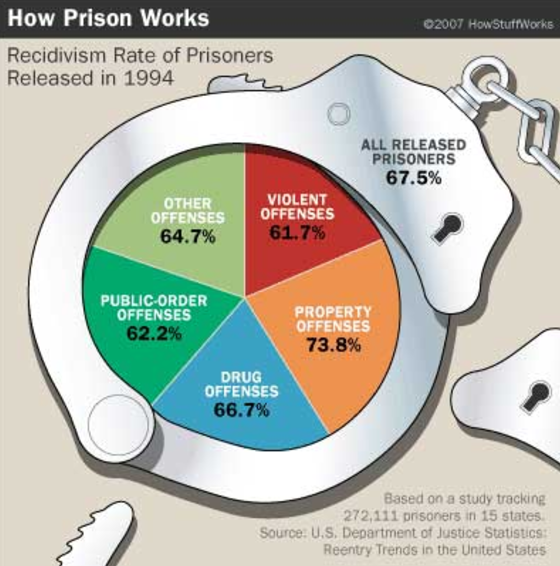
\includegraphics[width=0.5\textwidth,height=\textheight]{src/../images/badviz3.png}

}

\caption{Source: http://viz.wtf/}

\end{figure}%

\hfill\break
\hfill\break
\hfill\break

\begin{figure}[H]

{\centering 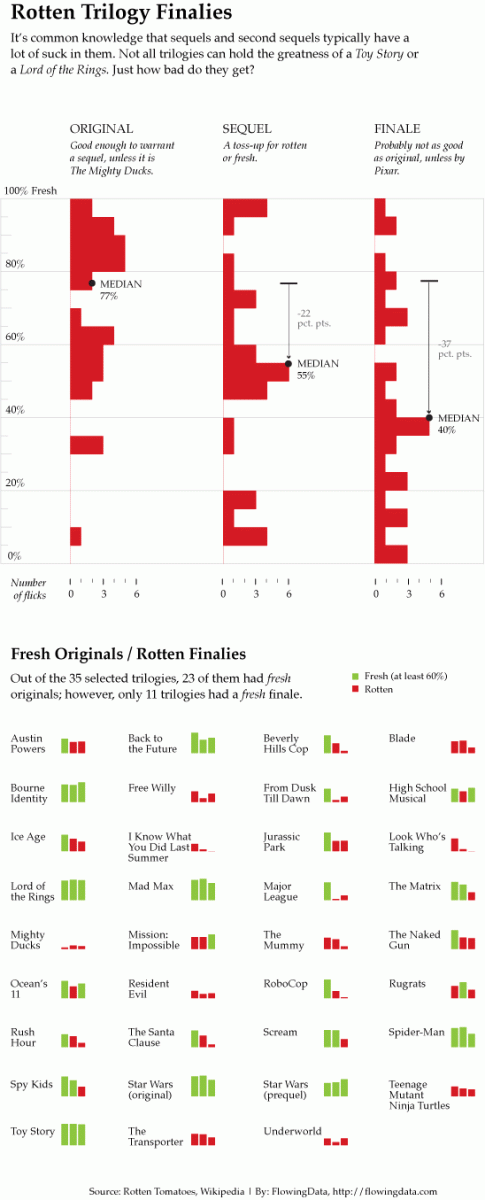
\includegraphics[width=0.5\textwidth,height=\textheight]{src/../images/trilogies.png}

}

\caption{Source: N. Yau, \emph{Visualize This}, 2011, p.~223-225.}

\end{figure}%

\hfill\break
\hfill\break
\hfill\break

\begin{figure}[H]

{\centering 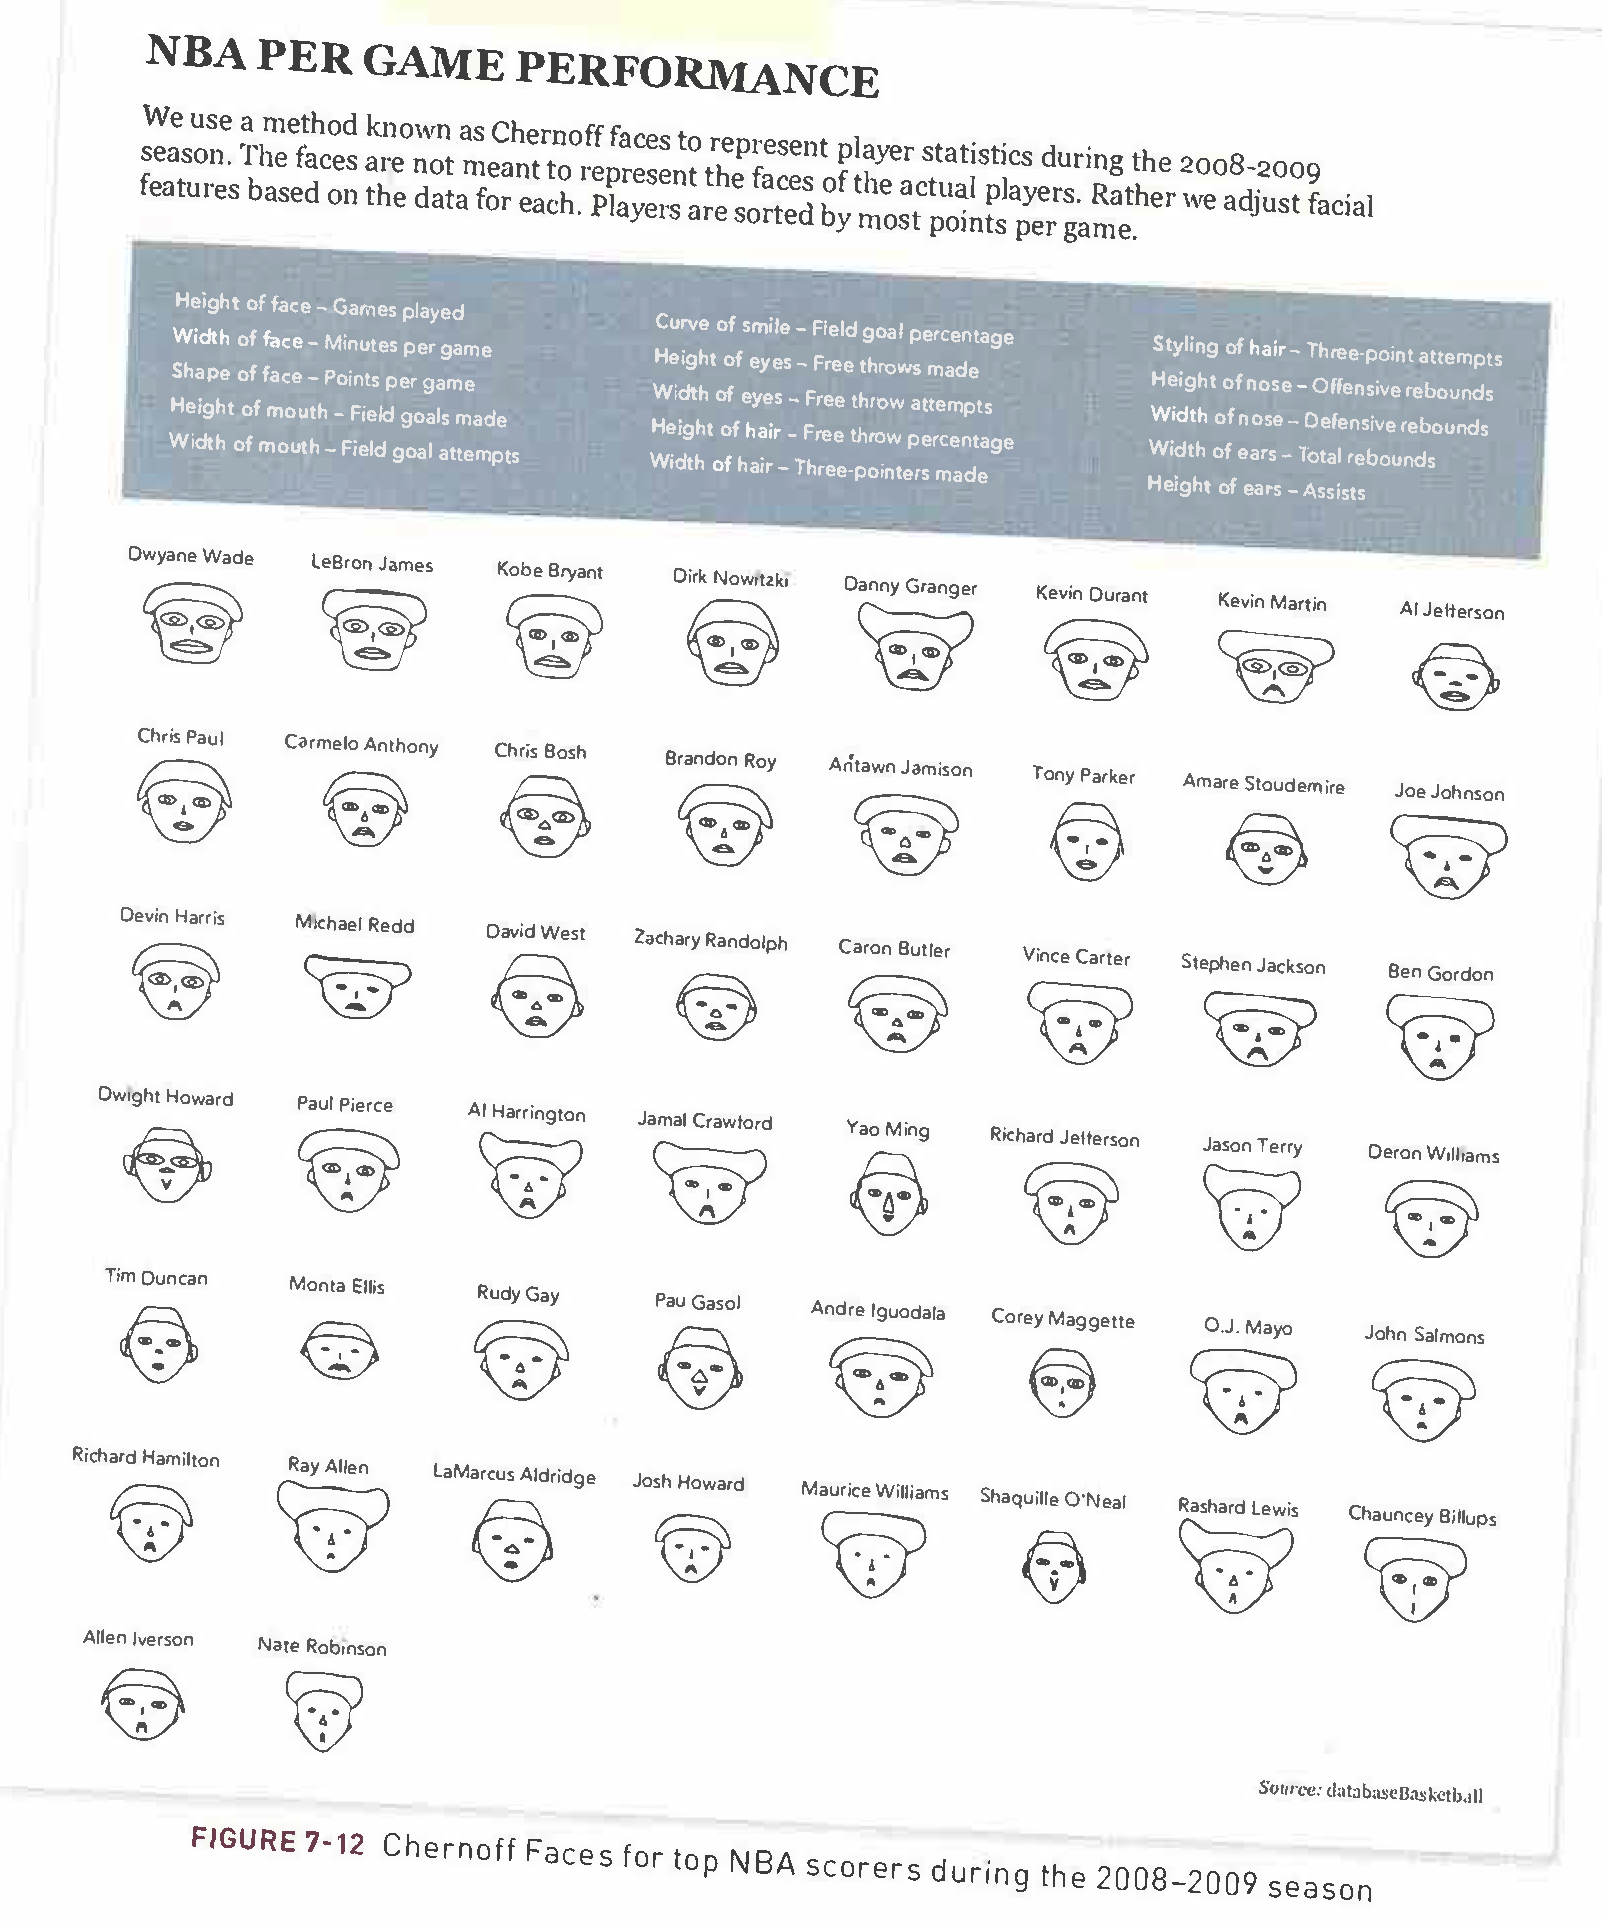
\includegraphics[width=0.6\textwidth,height=\textheight]{src/../images/chernoff.png}

}

\caption{Source: N. Yau, \emph{Visualize This}, 2011, p.~242.}

\end{figure}%

\hfill\break
\hfill\break
\hfill\break

\begin{figure}[H]

{\centering 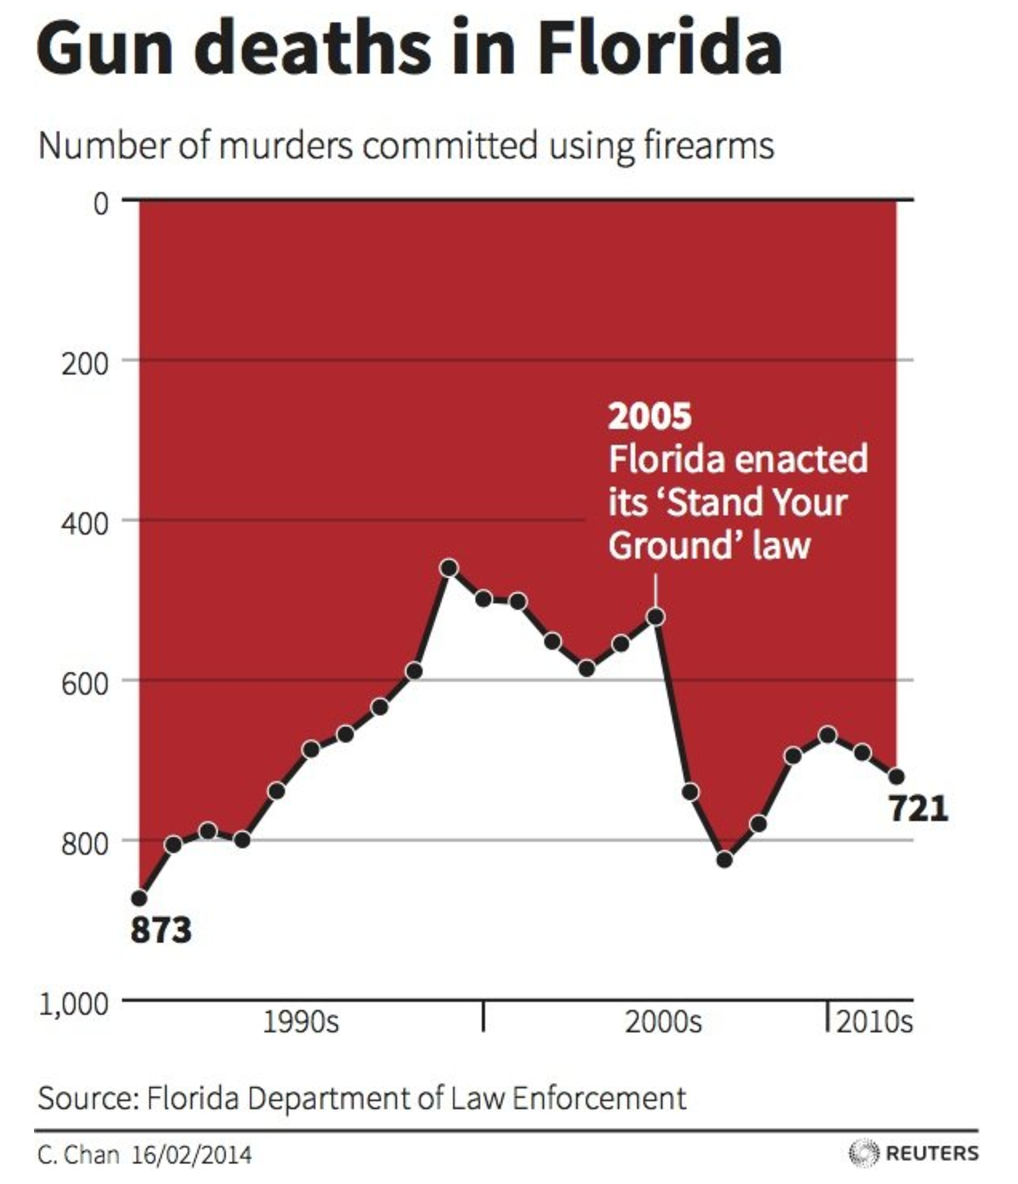
\includegraphics[width=0.7\textwidth,height=\textheight]{src/../images/badviz2.png}

}

\caption{Gun deaths.}

\end{figure}%

\hfill\break
\hfill\break
\hfill\break

\begin{figure}[H]

{\centering 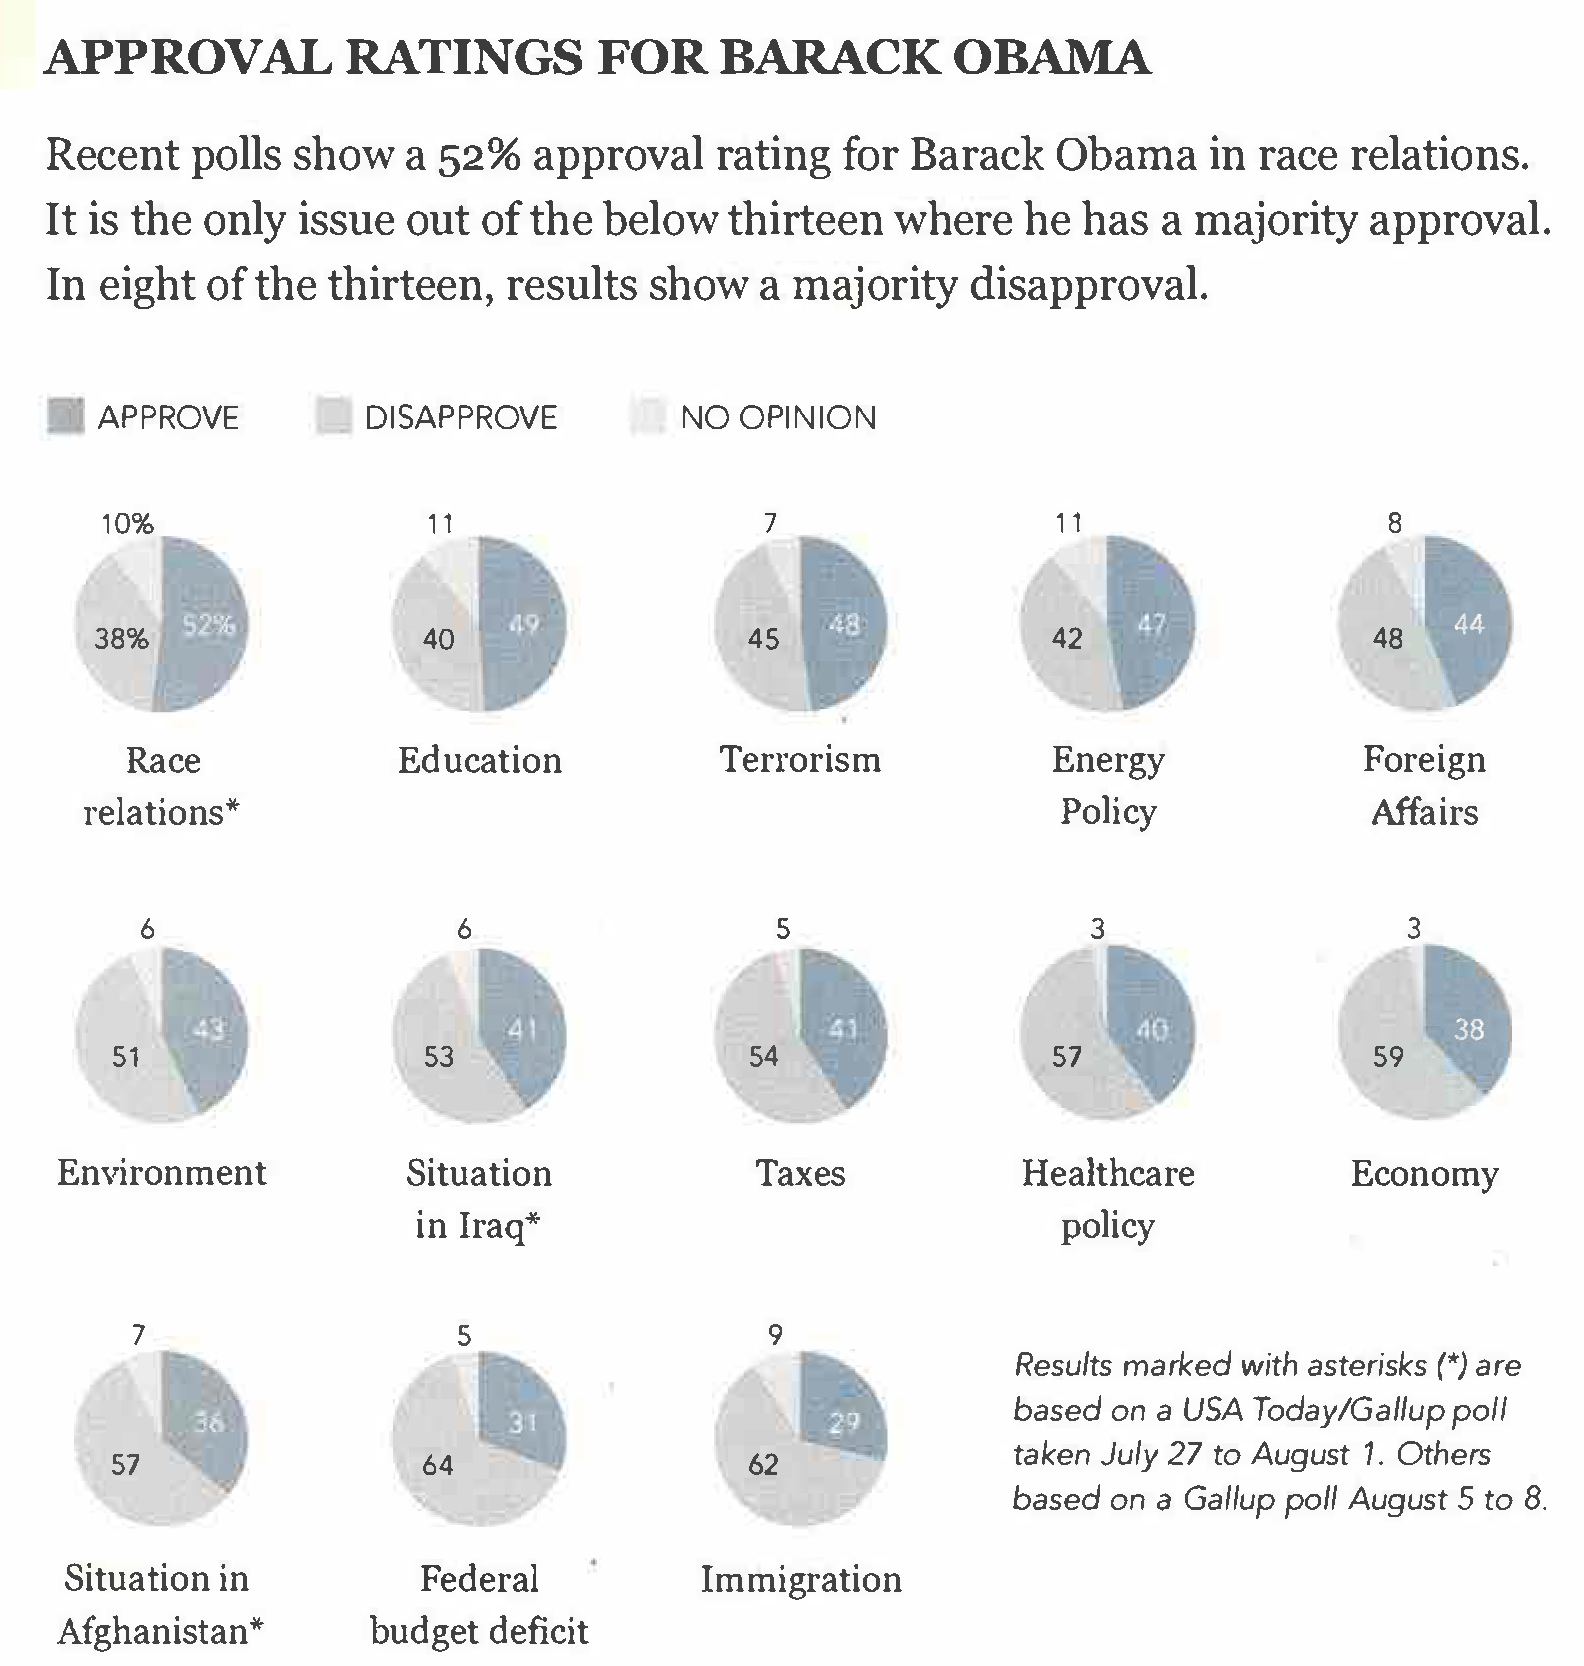
\includegraphics[width=0.8\textwidth,height=\textheight]{src/../images/obama1.png}

}

\caption{Source: N. Yau, \emph{Visualize This}, 2011, p.~150.}

\end{figure}%

\hfill\break
\hfill\break
\hfill\break

\begin{figure}[H]

{\centering 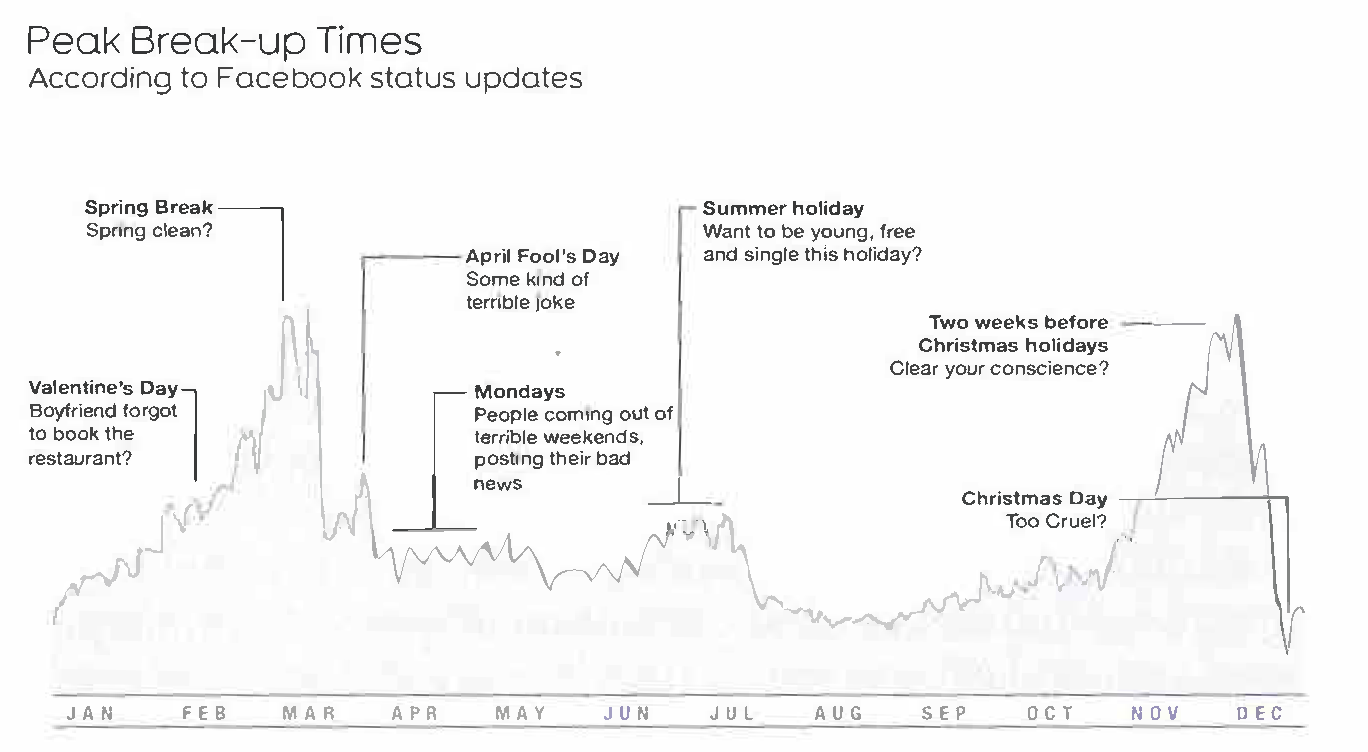
\includegraphics[width=0.8\textwidth,height=\textheight]{src/../images/breakup.png}

}

\caption{Source: C. N. Knaflic, \emph{Storytelling with Data}, 2015,
p.~142.}

\end{figure}%

\hfill\break
\hfill\break
\hfill\break

\begin{figure}[H]

{\centering 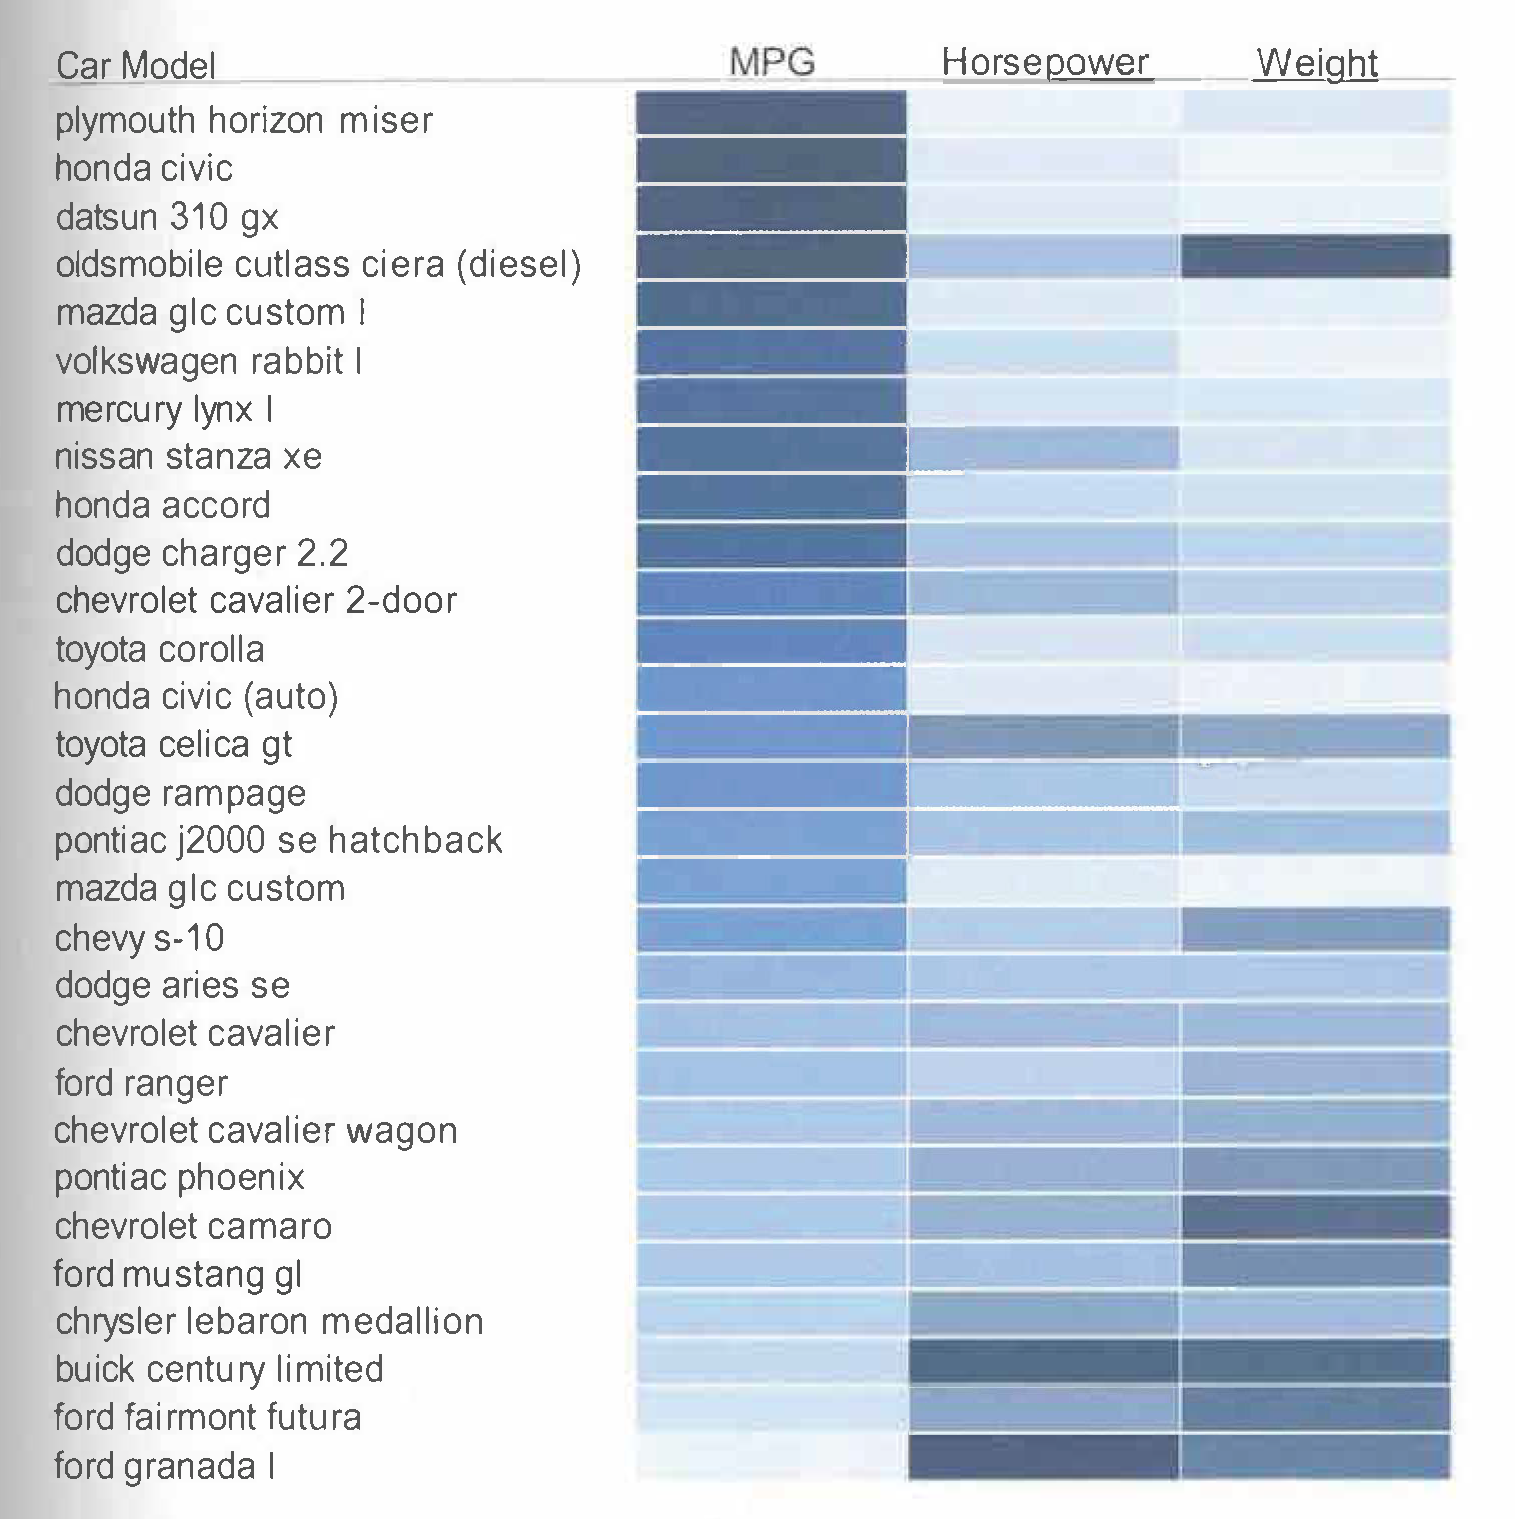
\includegraphics[width=0.6\textwidth,height=\textheight]{src/../images/heatmap.png}

}

\caption{Source: S. Few, \emph{Now You See It}, 2009, p.~45.}

\end{figure}%

\hfill\break
\hfill\break
\hfill\break

\begin{figure}[H]

{\centering 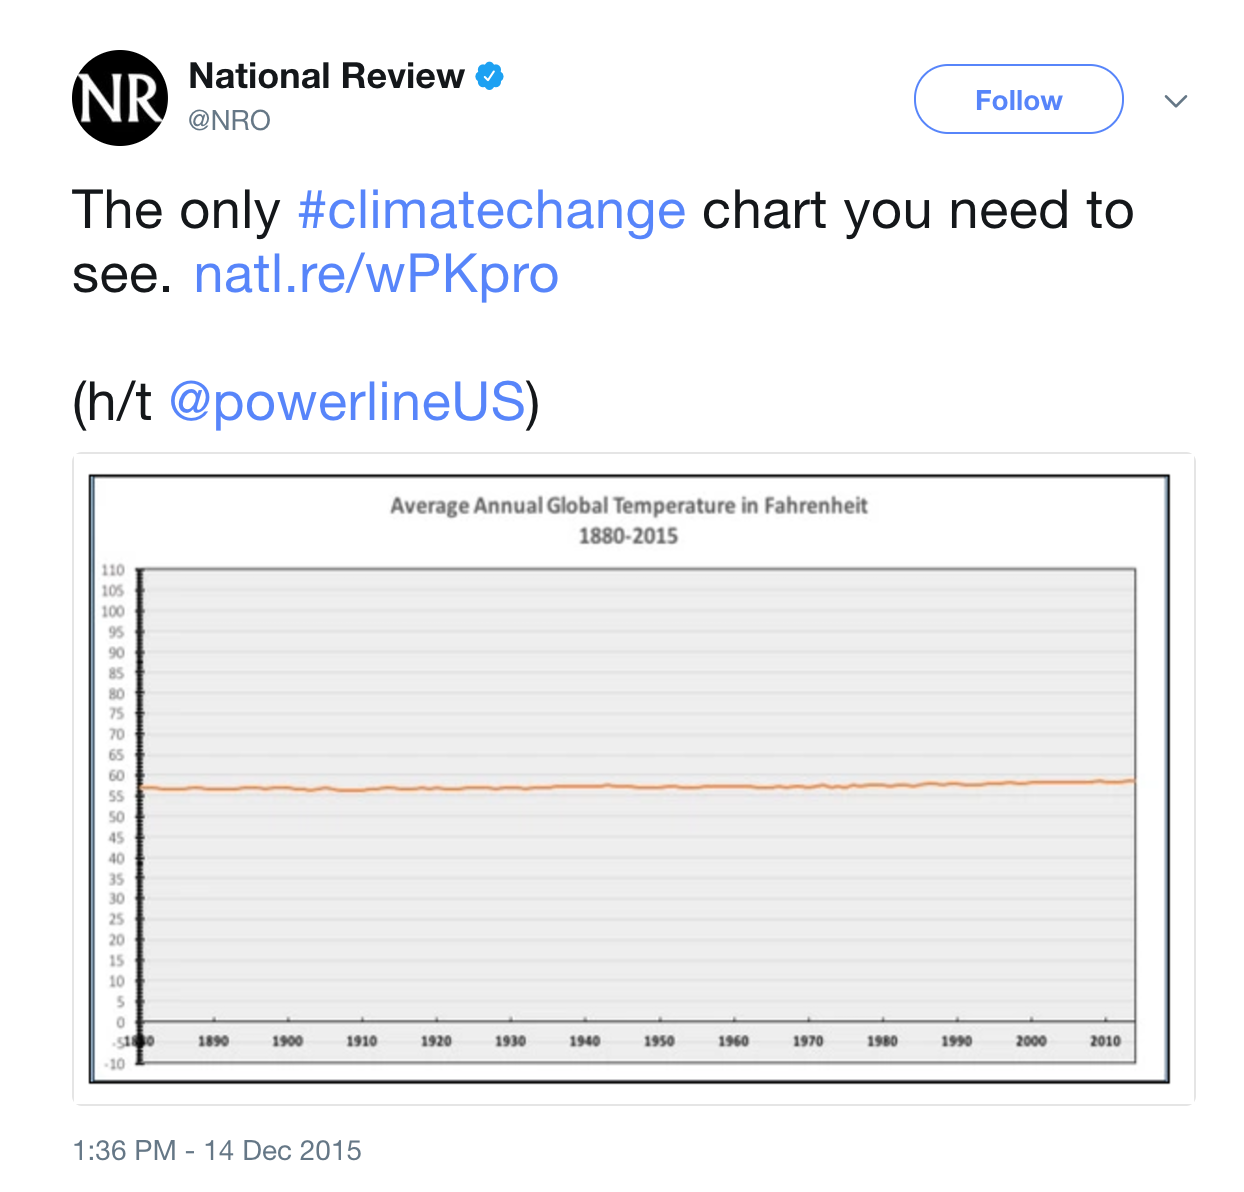
\includegraphics[width=0.6\textwidth,height=\textheight]{src/../images/badviz1.png}

}

\caption{Climate change.}

\end{figure}%

\hfill\break
\hfill\break
\hfill\break

\begin{figure}[H]

{\centering 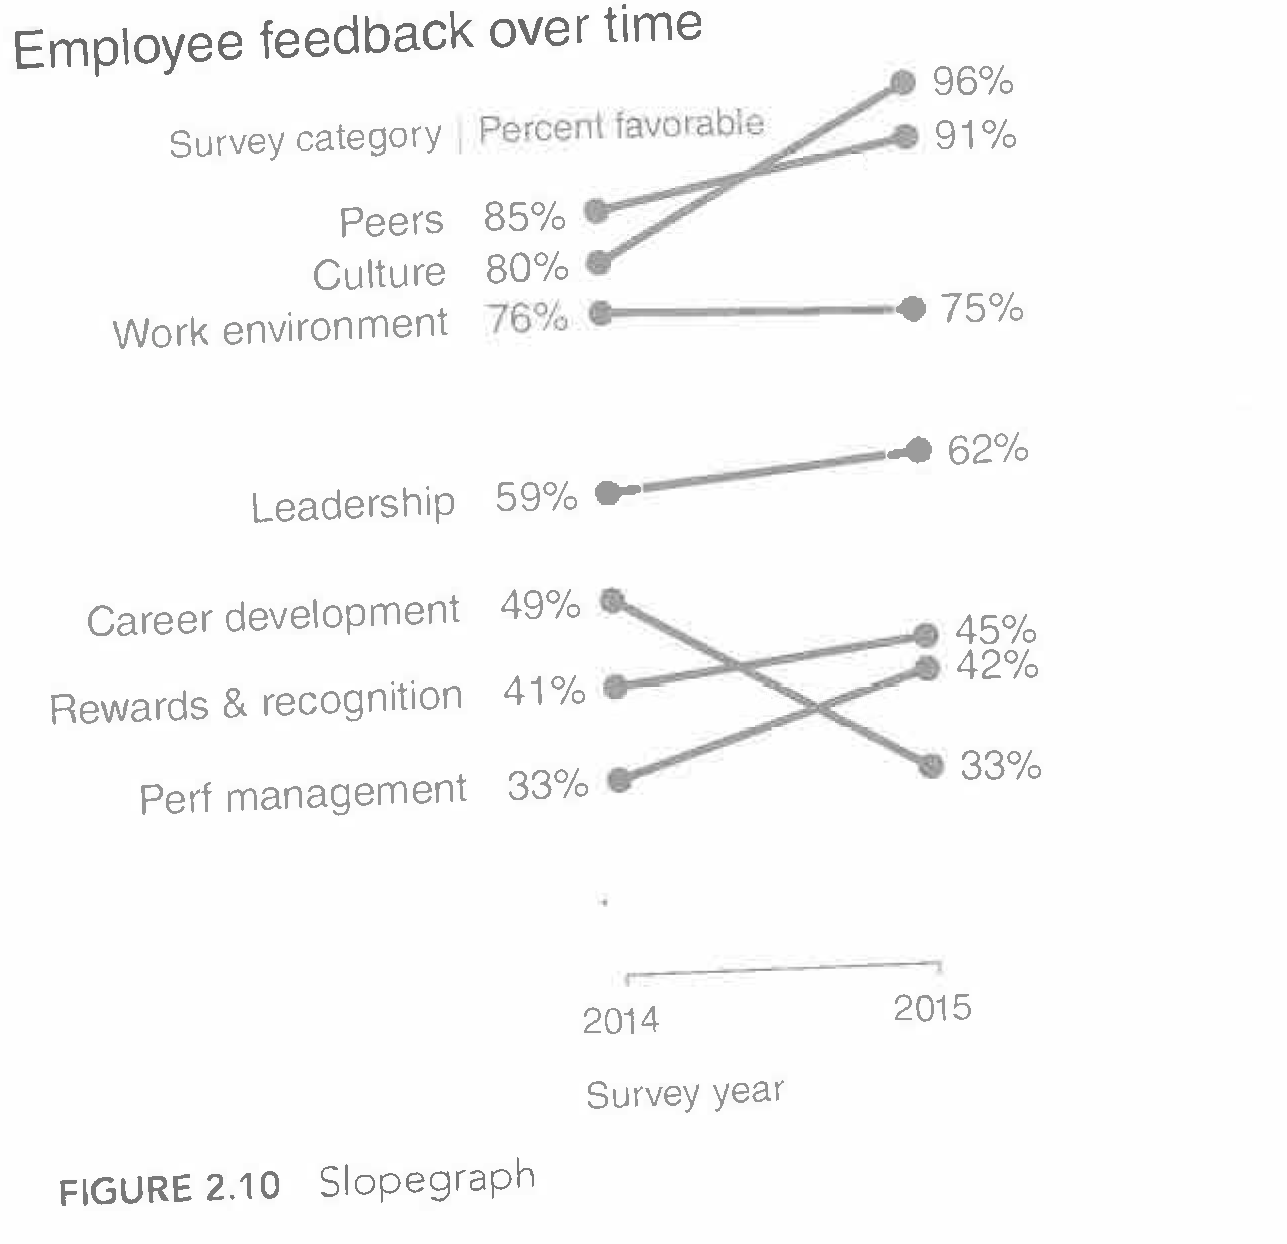
\includegraphics[width=0.5\textwidth,height=\textheight]{src/../images/slopegraph1.png}

}

\caption{Source: C. N. Knaflic, \emph{Storytelling with Data}, 2015,
p.~48.}

\end{figure}%

\hfill\break
\hfill\break
\hfill\break

\begin{figure}[H]

{\centering 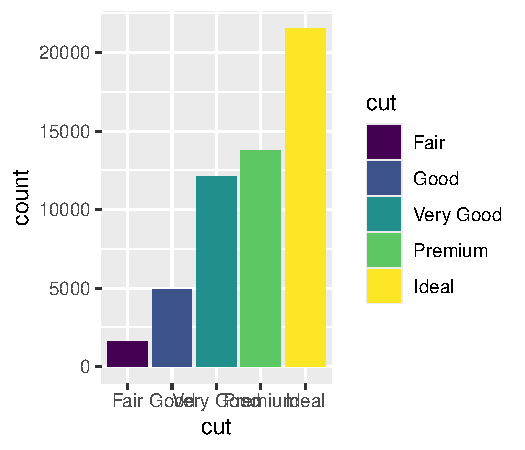
\includegraphics{src/03-Effective_Viz_files/figure-pdf/unnamed-chunk-11-1.pdf}

}

\caption{Diamond data visualizations from
\href{http://r4ds.had.co.nz/data-visualisation.html\#position-adjustments}{\emph{R
for Data Science}}, 2017}

\end{figure}%

\begin{figure}[H]

{\centering 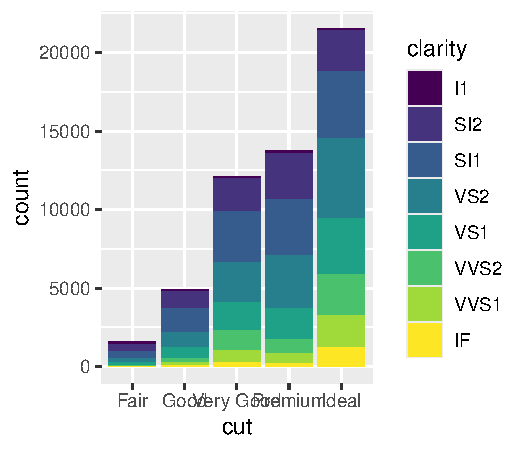
\includegraphics{src/03-Effective_Viz_files/figure-pdf/unnamed-chunk-11-2.pdf}

}

\caption{Diamond data visualizations from
\href{http://r4ds.had.co.nz/data-visualisation.html\#position-adjustments}{\emph{R
for Data Science}}, 2017}

\end{figure}%

\begin{figure}[H]

{\centering 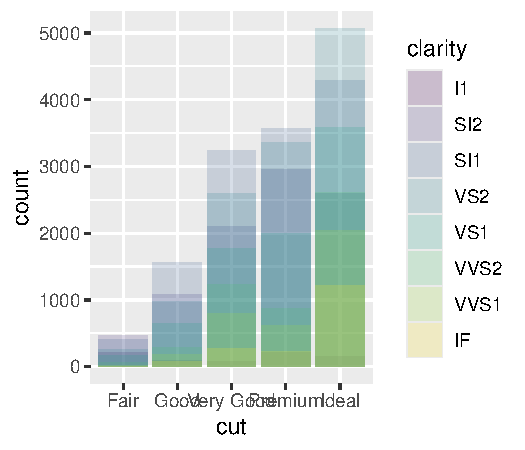
\includegraphics{src/03-Effective_Viz_files/figure-pdf/unnamed-chunk-11-3.pdf}

}

\caption{Diamond data visualizations from
\href{http://r4ds.had.co.nz/data-visualisation.html\#position-adjustments}{\emph{R
for Data Science}}, 2017}

\end{figure}%

\begin{figure}[H]

{\centering 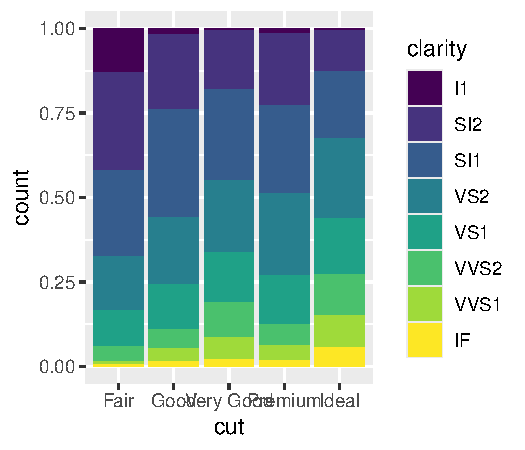
\includegraphics{src/03-Effective_Viz_files/figure-pdf/unnamed-chunk-11-4.pdf}

}

\caption{Diamond data visualizations from
\href{http://r4ds.had.co.nz/data-visualisation.html\#position-adjustments}{\emph{R
for Data Science}}, 2017}

\end{figure}%

\begin{figure}[H]

{\centering 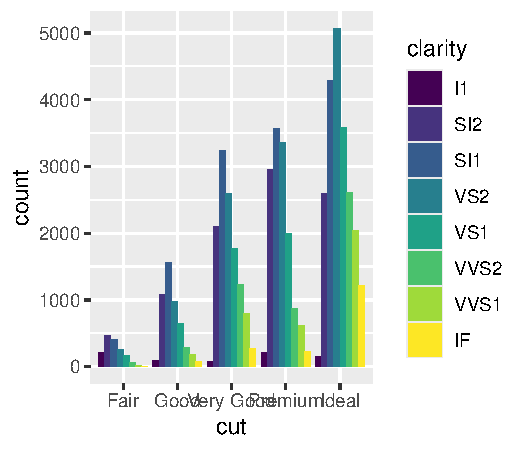
\includegraphics{src/03-Effective_Viz_files/figure-pdf/unnamed-chunk-11-5.pdf}

}

\caption{Diamond data visualizations from
\href{http://r4ds.had.co.nz/data-visualisation.html\#position-adjustments}{\emph{R
for Data Science}}, 2017}

\end{figure}%

\hfill\break
\hfill\break
\hfill\break

\begin{figure}[H]

{\centering 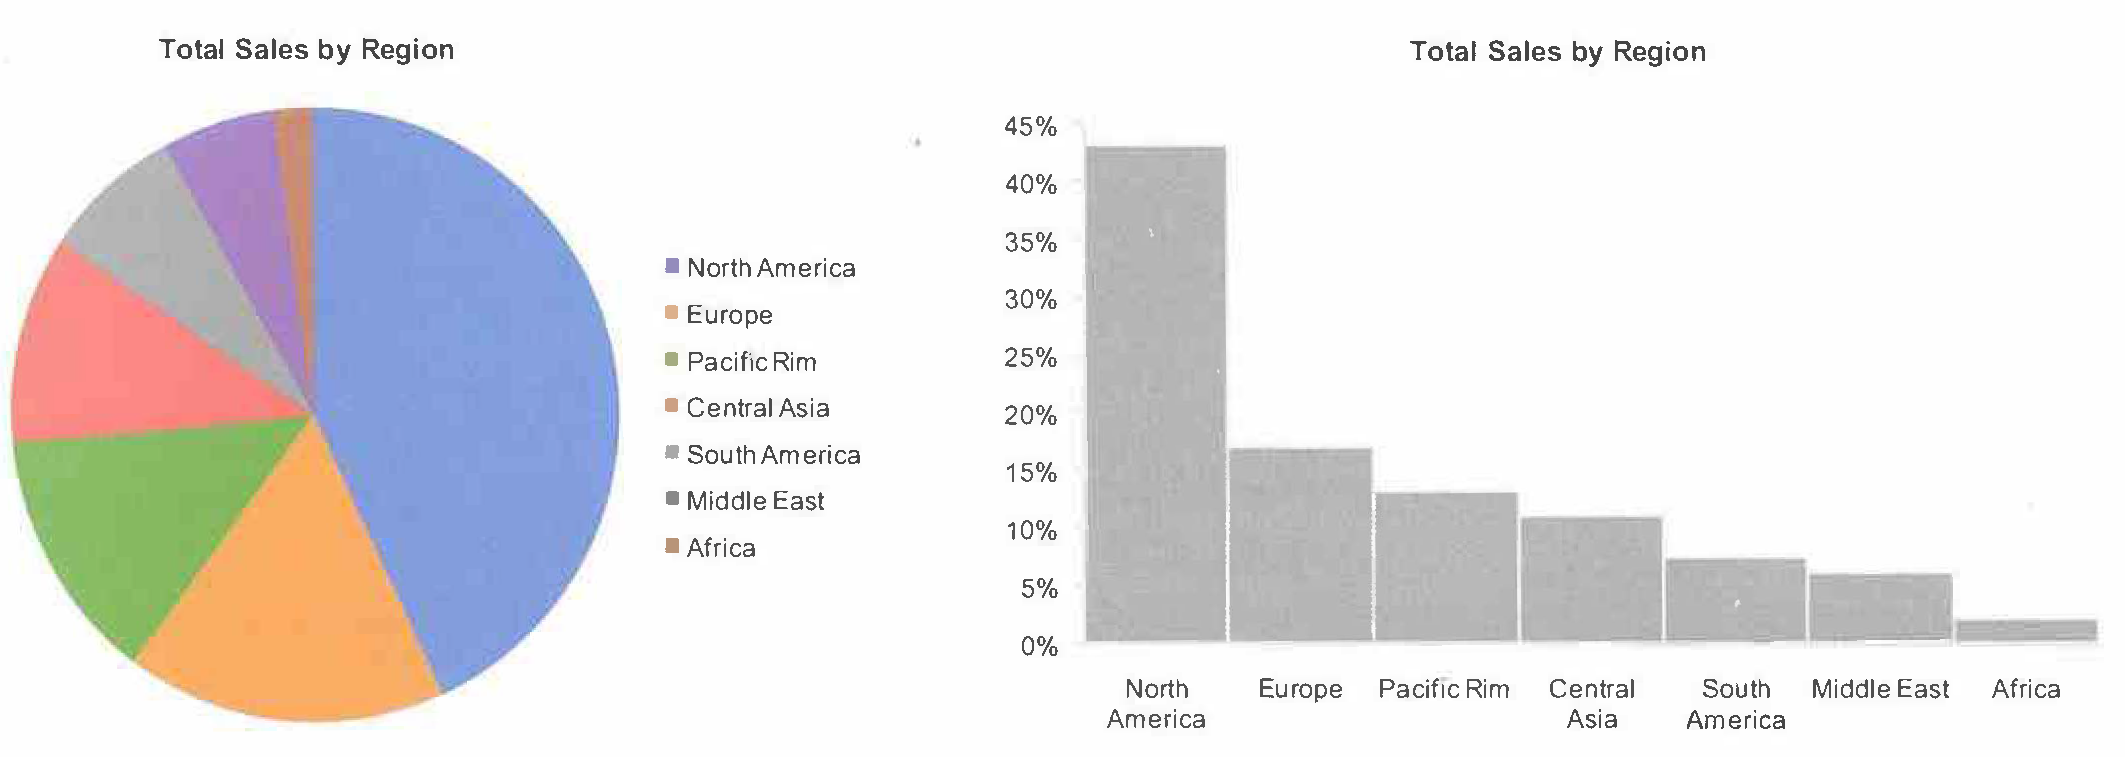
\includegraphics[width=1\textwidth,height=\textheight]{src/../images/piechart.png}

}

\caption{Source: S. Few, \emph{Now You See It}, 2009, p.~37.}

\end{figure}%

\hfill\break
\hfill\break
\hfill\break

\begin{figure}[H]

{\centering 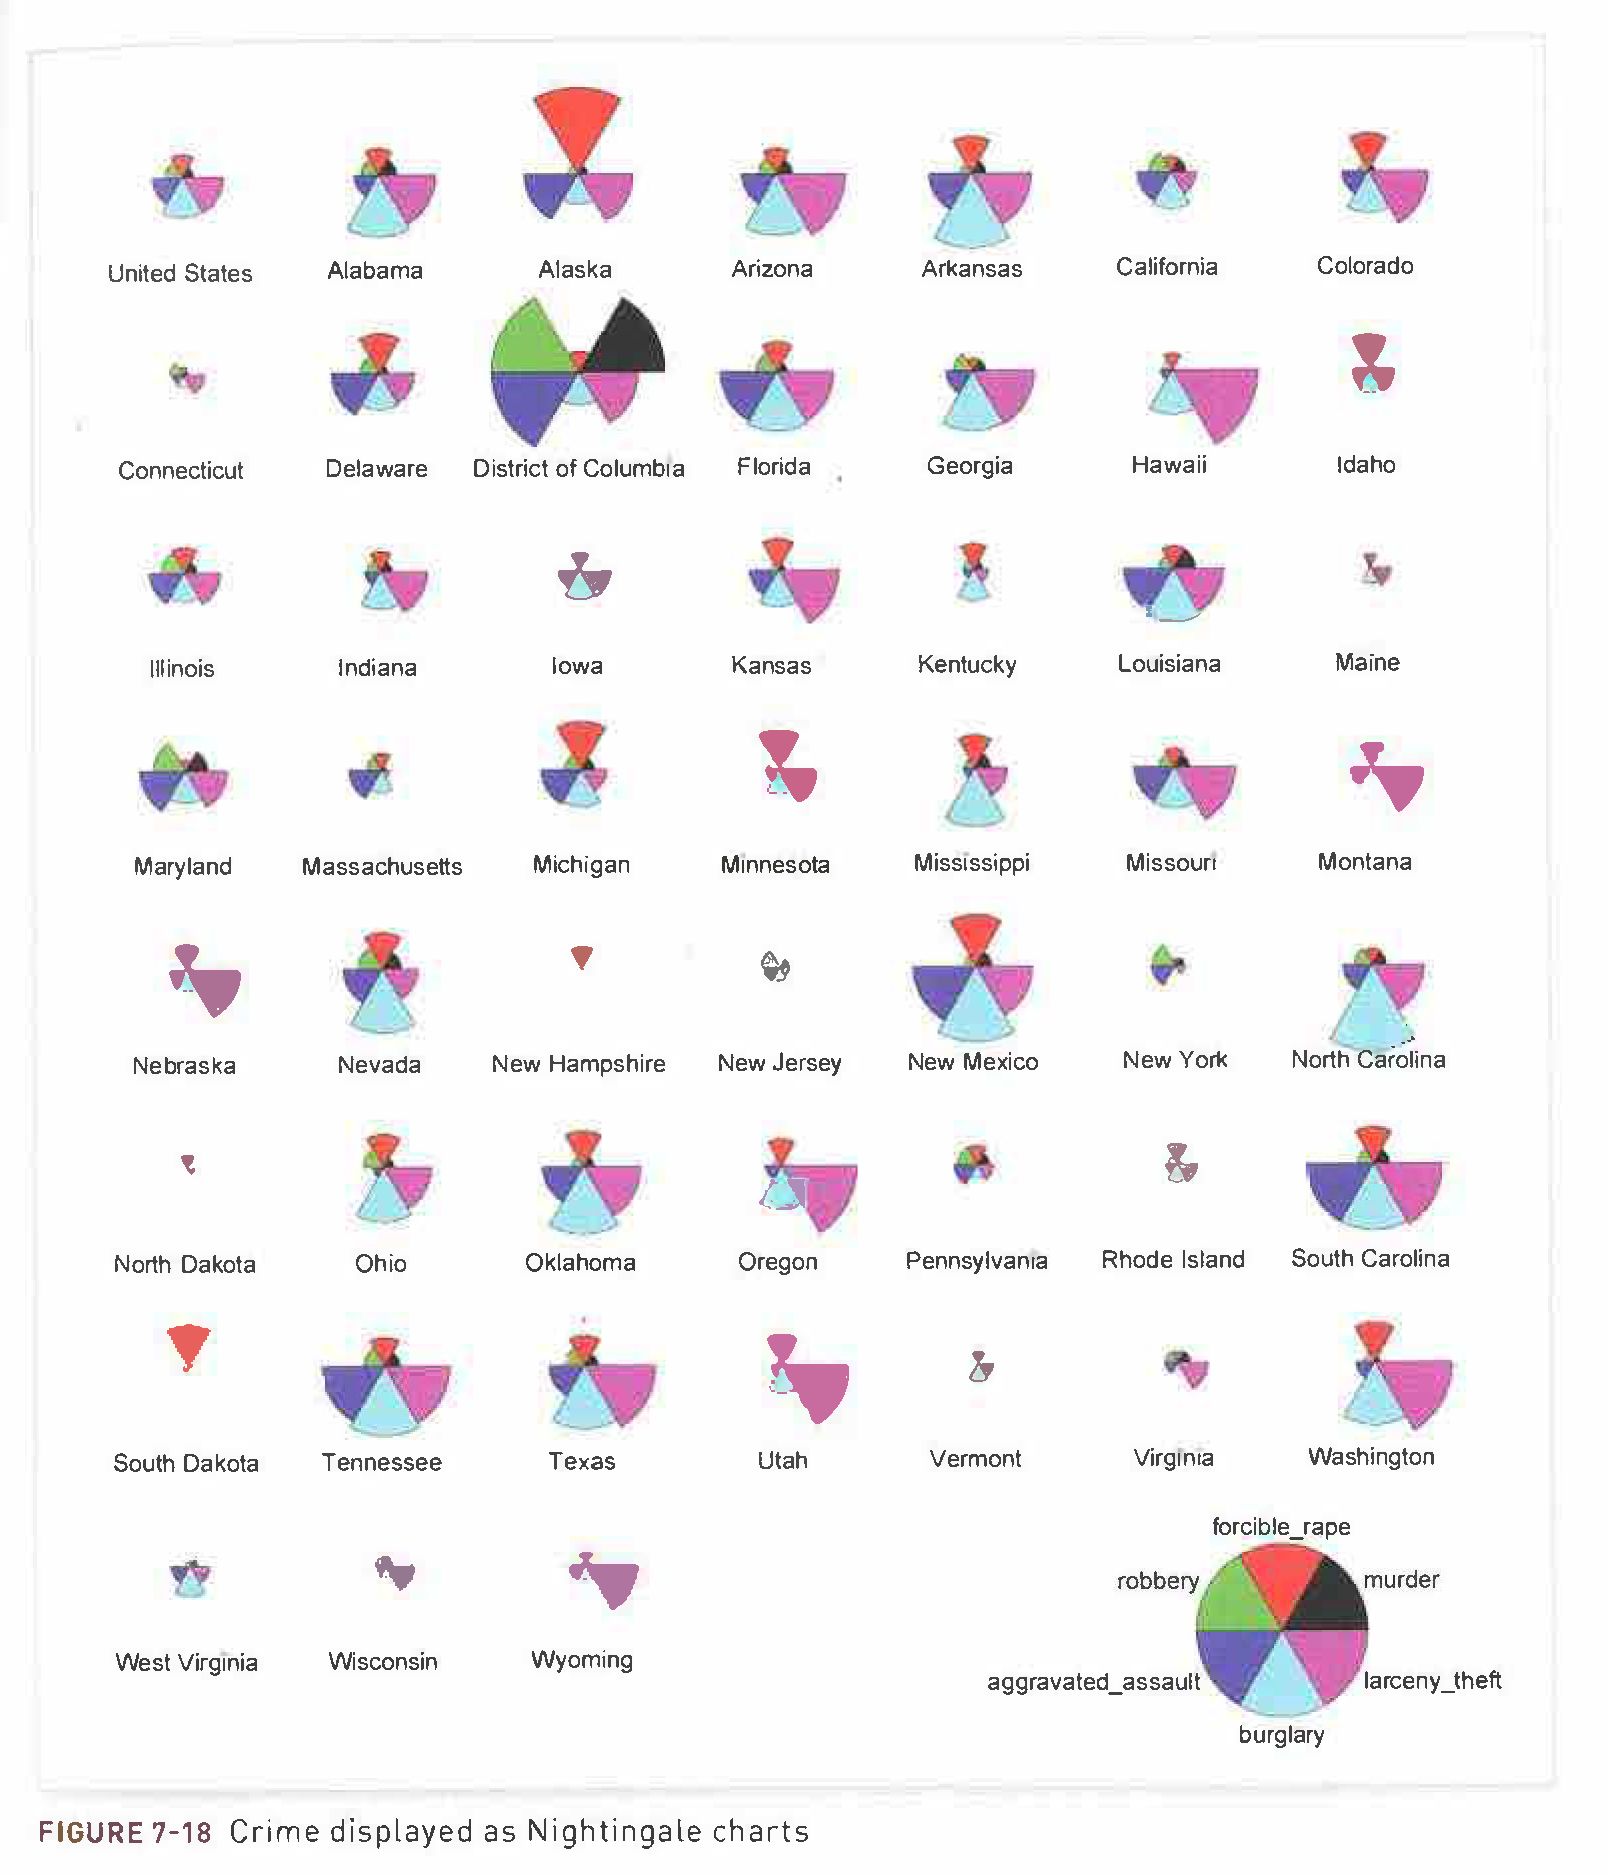
\includegraphics[width=0.7\textwidth,height=\textheight]{src/../images/Nightingale.png}

}

\caption{Source: N. Yau, \emph{Visualize This}, 2011, p.~249.}

\end{figure}%

\hfill\break
\hfill\break
\hfill\break

\begin{figure}[H]

{\centering \includegraphics[width=0.8\textwidth,height=\textheight]{src/../images/compensation.png}

}

\caption{Source: S. Few, \emph{Now You See It}, 2009, p.~61.}

\end{figure}%

\hfill\break
\hfill\break
\hfill\break

\begin{figure}[H]

{\centering \includegraphics[width=1\textwidth,height=\textheight]{src/../images/employees.png}

}

\caption{Source: C. N. Knaflic, \emph{Storytelling with Data}, 2015,
p.~68.}

\end{figure}%

\hfill\break
\hfill\break
\hfill\break

\begin{figure}[H]

{\centering \includegraphics[width=0.7\textwidth,height=\textheight]{src/../images/clutter.png}

}

\caption{Source: C. N. Knaflic, \emph{Storytelling with Data}, 2015,
p.~81.}

\end{figure}%

\hfill\break
\hfill\break
\hfill\break

\begin{figure}[H]

{\centering \includegraphics[width=0.6\textwidth,height=\textheight]{src/../images/badviz4.png}

}

\caption{Source: http://viz.wtf/}

\end{figure}%

\hfill\break
\hfill\break
\hfill\break

\begin{figure}[H]

{\centering \includegraphics[width=0.85\textwidth,height=\textheight]{src/../images/plagiarism.png}

}

\caption{Source: A. Cairo, \emph{The Functional Art}, 2013, p.~340.}

\end{figure}%

\hfill\break
\hfill\break
\hfill\break

\begin{figure}[H]

{\centering \includegraphics[width=0.7\textwidth,height=\textheight]{src/../images/tv-size-by-year1.png}

}

\caption{Source: N. Yau, \emph{Visualize This}, 2011, p.~220.}

\end{figure}%

\hfill\break
\hfill\break
\hfill\break

\textbf{More examples}:

\begin{itemize}
\tightlist
\item
  FlowingData: \href{http://flowingdata.com/}{blog} and
  \href{https://flowingdata.com/2016/12/29/best-data-visualization-projects-of-2016/}{Best
  visualizations of 2016}
\item
  \href{http://viz.wtf/}{WTF Visualizations}
\end{itemize}

\subsection*{Properties of Effective
Visualizations}\label{properties-of-effective-visualizations}
\addcontentsline{toc}{subsection}{Properties of Effective
Visualizations}

\subsubsection*{Storytelling / Context}\label{storytelling-context}
\addcontentsline{toc}{subsubsection}{Storytelling / Context}

Remember \ldots{}

\begin{quote}
Graphics are designed by the human expert (you!) in order to reveal
information that's in the data.
\end{quote}

Your choices depend on what information you want to reveal and convey.
So before you complete a graphic, you should clearly identify what story
you want the graphic to tell to the audience, and double check that this
story is being told.\footnote{A ``negative'' result (e.g., there is no
  correlation between two variables) is a perfectly fine story to tell.}

\href{https://fivethirtyeight.com/features/six-charts-to-help-americans-understand-the-upcoming-german-election/}{Here}
is a nice example from \texttt{FiveThirtyEight} where each chart tells a
story in answer to a particular question about the {[}then{]} upcoming
German election.

\href{https://fivethirtyeight.com/features/gun-deaths/}{Here} is an
interactive visualization that tells a story about gun violence.

Another important contextual question to ask is whether the graphic is
for an explanatory (\emph{explain why}) or exploratory
(\emph{discovering something new}) analysis.

\subsubsection*{Accessibility}\label{accessibility}
\addcontentsline{toc}{subsubsection}{Accessibility}

In addition to considering the story you are telling, you need to
consider what audiences can access your story.

\textbf{Alternative (Alt) Text}: In order for data visualizations to be
accessible to people who are blind and use screen readers, we can
provide alt text. Alt text should concisely articulate (1) what your
visualization is (e.g.~a bar chart showing which the harvest rate of
cucumbers), (2) a one sentence description of the what you think is the
most important takeaway your visualization is showing, and (3) a link to
your data source if it's not already in the caption (check out this
\href{https://medium.com/nightingale/writing-alt-text-for-data-visualization-2a218ef43f81}{great
resource on writing alt text for data visualizations}).

To add the alt text to your the HTML created from knitting the Rmd, you
can include it as an option at the top of your r chunk. For example:
\{r, fig.alt = ``Bar chart showing the daily harvest of cucumbers. The
peak cucumber collection day is August 18th''\}. To see the alt text in
the knitted html file, you can hover over the image.

\textbf{Color-blind friendly color palettes}: In order for data
visualizations to be accessible to people with
\href{https://www.nei.nih.gov/learn-about-eye-health/eye-conditions-and-diseases/color-blindness\#:~:text=What\%20is\%20color\%20blindness\%3F,and\%20contact\%20lenses\%20can\%20help.}{color
blindness}, we need to be thoughtful about the colors we use in our data
visualizations. The most common variety of color-blindness makes it hard
for individuals to detect differences between red and green. Some types
make it hard detect differences between blue and yellow. Other types
make it hard to see different shades of a color.

This \href{https://asada.website/webCVS/}{Chromatic Vision Simulator}
can give you a sense of how this could impact your perception of colors
(see image below). You could also upload a visualization to this
simulator to see how well your chosen color palette works.

\includegraphics[width=5.42in,height=\textheight]{src/../images/colorblind.jpg}

Try to use a color-blind friendly / safe palette whenever possible. One
easy way to do this is to include \texttt{+\ scale\_fill\_viridis\_d()}
or \texttt{+\ scale\_color\_viridis\_d()} when you are filling or
coloring by a discrete or categorical variable and
\texttt{+\ scale\_fill\_viridis\_c()} or
\texttt{+\ scale\_color\_viridis\_c()} when you are filling or coloring
by a continuous or quantitative variable. There are many other
color-blind friendly palettes in R; you can check out other resources
\href{https://cran.r-project.org/web/packages/colorBlindness/vignettes/colorBlindness.html}{here}.

\subsubsection*{Ethics}\label{ethics}
\addcontentsline{toc}{subsubsection}{Ethics}

Michael Correll of Tableau Research writes ``Data visualizations have a
potentially enormous influence on how data are used to make decisions
across all areas of human endeavor.'' in his
\href{https://arxiv.org/pdf/1811.07271.pdf}{article from 2018}.

Visualization operates at the intersection of science, communication,
and data science \& statistics. There are professional standards of
ethics in these fields of the power they hold over other people as it
relates to making data-driven decisions.

Correll describes three ethical challenges of visualization work:

\begin{enumerate}
\def\labelenumi{\arabic{enumi}.}
\tightlist
\item
  \textbf{Visibility} Make the invisible visible
\end{enumerate}

\begin{itemize}
\tightlist
\item
  Visualize hidden labor
\item
  Visualize hidden uncertainty
\item
  Visualize hidden impacts
\end{itemize}

\emph{Visualizations can be complex and one must consider the
accessibility of the visualization to the audience. Managing complexity
is, therefore, a virtue in design that can be in direct opposition with
the desire to visualize the invisible.}

\begin{enumerate}
\def\labelenumi{\arabic{enumi}.}
\setcounter{enumi}{1}
\tightlist
\item
  \textbf{Privacy} Collect data with empathy
\end{enumerate}

\begin{itemize}
\tightlist
\item
  Encourage Small Data
\item
  Anthropomorphize data
\item
  Obfuscate data to protect privacy
\end{itemize}

\emph{Restricting the type and amount of data that is collected has a
direct impact on the quality and scope of the analyses hence obligation
to provide context, and analytical power can, therefore, stand in direct
opposition to the empathic collection of data.}

\begin{enumerate}
\def\labelenumi{\arabic{enumi}.}
\setcounter{enumi}{2}
\tightlist
\item
  \textbf{Power} Challenge structures of power
\end{enumerate}

\begin{itemize}
\tightlist
\item
  Support data due process.
\item
  Act as data advocates.
\item
  Pressure unethical analytical behavior.
\end{itemize}

\emph{The goal of promoting truth and suppressing falsehood may require
amplifying existing structures of expertise and power, and suppressing
conflicts for the sake of rhetorical impact.}

At a minimum, you should always

\begin{enumerate}
\def\labelenumi{\arabic{enumi}.}
\item
  Present data in a way that avoids misleading the audience.
\item
  Always include your data source. Doing so attributes credit for labor,
  provides credibility to your work, and provides context for your
  graphic.
\end{enumerate}

\subsubsection*{Design}\label{design}
\addcontentsline{toc}{subsubsection}{Design}

A basic principle is that a graphic is about \emph{comparison}. Good
graphics make it easy for people to perceive things that are similar and
things that are different. Good graphics put the things to be compared
``side-by-side,'' that is, in perceptual proximity to one another. The
following aesthetics are listed in roughly descending order of human
ability to perceive and compare nearby objects:\footnote{This list is
  from B. S. Baumer, D. T. Kaplan, and N. J. Horton, \emph{Modern Data
  Science with R}, 2017, p.~15. For more of the theory of perception,
  see also W.S. Cleveland and R. McGill,
  ``\href{http://www.math.pku.edu.cn/teachers/xirb/Courses/biostatistics/Biostatistics2016/GraphicalPerception_Jasa1984.pdf}{Graphical
  perception: Theory, experimentation, and application to the
  development of graphical methods},'' \emph{Journal of the American
  Statistical Association}, 1984.}

\begin{enumerate}
\def\labelenumi{\arabic{enumi}.}
\tightlist
\item
  Position
\item
  Length
\item
  Angle
\item
  Direction
\item
  Shape (but only a very few different shapes)
\item
  Area
\item
  Volume
\item
  Shade
\item
  Color
\end{enumerate}

Color is the most difficult, because it is a 3-dimensional quantity. We
are pretty good at color gradients, but discrete colors must be selected
carefully. We need to be particularly aware of red/green color blindness
issues.

\textbf{Visual perception and effective visualizations}

Here are some facts to keep in mind about visual perception from
\href{https://www.amazon.com/Now-You-See-Visualization-Quantitative/dp/0970601980}{Now
You See It}:

\begin{enumerate}
\def\labelenumi{\arabic{enumi}.}
\tightlist
\item
  Visual perception is selective, and our attention is often drawn to
  constrasts from the norm.
\end{enumerate}

\begin{figure}[H]

{\centering \includegraphics[width=1\textwidth,height=\textheight]{src/../images/contrast.png}

}

\caption{Our attention is drawn to contrasts to the norm. What stands
out in this example image?, which is originally from C. Ware,
\emph{Information Visualization: Perception for Design}, 2004? Source:
S. Few, \emph{Now You See It}, 2009, p.~33.}

\end{figure}%

\begin{quote}
\textbf{Implication}: We should design visualizations so that the
features we want to highlight stand out in contrast from those that are
not worth the audience's attention.
\end{quote}

\begin{enumerate}
\def\labelenumi{\arabic{enumi}.}
\setcounter{enumi}{1}
\tightlist
\item
  Our eyes are drawn to familiar patterns. We see what we know and
  expect.
\end{enumerate}

\begin{figure}[H]

{\centering \includegraphics[width=0.9\textwidth,height=\textheight]{src/../images/rose1.png}

}

\caption{Do you see anything embedded in this rose image from
coolbubble.com? Source: S. Few, \emph{Now You See It}, 2009, p.~34.}

\end{figure}%

\begin{quote}
\textbf{Implication}: Visualizations work best when they display
information as patterns that familiar and easy to spot.
\end{quote}

\begin{enumerate}
\def\labelenumi{\arabic{enumi}.}
\setcounter{enumi}{2}
\tightlist
\item
  Memory plays an important role in human cognition, but working memory
  is extremely limited.
\end{enumerate}

\begin{quote}
\textbf{Implication}: Visualizations must serve as external aids to
augment working memory. If a visualization is unfamiliar, then it won't
be as effective.
\end{quote}

\textbf{Gestalt principles}

The Gestalt principles (more info
\href{https://en.wikipedia.org/wiki/Principles_of_grouping}{here} or
\href{https://www.smashingmagazine.com/2014/03/design-principles-visual-perception-and-the-principles-of-gestalt/}{here})
were developed by psychologists including Max Wertheimer in the early
1900s to explain how humans perceive organized patterns and objects.

In a design setting, they help us understand how to incorporate
\textbf{preattentive features} into visualizations. The figure below
shows some preattentive features, all of which are processed prior to
conscious attention (``at a glance'') and can help the reader focus on
relevant information in a visualization.

\begin{figure}[H]

{\centering \includegraphics[width=1\textwidth,height=\textheight]{src/../images/gestalt.png}

}

\caption{Preattentive features based on the Gestalt principles. Source:
I. Meirelles, \emph{Design for Information}, 2013, p.~23.}

\end{figure}%

\textbf{Other design tips} from
\href{https://www.amazon.com/Visualize-This-FlowingData-Visualization-Statistics/dp/0470944889/}{Visualize
This} and
\href{https://www.amazon.com/Storytelling-Data-Visualization-Business-Professionals/dp/1119002257}{Storytelling
with Data}:

\begin{itemize}
\tightlist
\item
  Put yourself in a reader's shoes when you design data graphics. What
  parts of the data need explanation? We can minimize ambiguity by
  providing guides, label axes, etc.
\item
  Data graphics are meant to shine a light on your data. Try to remove
  any elements that don't help you do that. That is, eliminate ``chart
  junk'' (distracting and unnecessary adornments).
\item
  Vary color and stroke styles to emphasize the parts in your graphic
  that are most important to the story you're telling
\item
  It is easier to judge length than it is to judge area or angles
\item
  Be thoughtful about how your categories (levels) are ordered for
  categorical data. There may be a natural ordering
\item
  Pie charts, donut charts, and 3D are evil
\end{itemize}

\subsection*{Basic Rules for Constructing
Graphics}\label{basic-rules-for-constructing-graphics}
\addcontentsline{toc}{subsection}{Basic Rules for Constructing Graphics}

Instead of memorizing which plot is appropriate for which situation,
it's best to simply start to recognize patterns in constructing
graphics:

\begin{itemize}
\tightlist
\item
  Each quantitative variable requires a new axis.\\
\item
  Each categorical variable requires a new way to ``group'' the graphic
  (eg: using colors, shapes, separate facets, etc to capture the
  grouping).
\item
  For visualizations in which overlap in glyphs or plots obscures the
  patterns, try faceting or transparency.
\end{itemize}

\subsection*{Still to Come}\label{still-to-come}
\addcontentsline{toc}{subsection}{Still to Come}

While we will not cover all of visualization theory -- you can take a
whole course on that at Macalester and it is a proper field in its own
right -- we will touch on the following types of visualizations in the
coming weeks:

\begin{itemize}
\tightlist
\item
  Bivariate visualizations
\item
  Visualizations of higher dimensional data
\item
  Temporal structures: timelines and flows
\item
  Hierarchical structures: trees
\item
  Relational structures: networks
\item
  Spatial structures: maps
\item
  Spatio-temporal structures
\item
  Textual structures
\item
  Interactive graphics (e.g., \texttt{gganimate}, \texttt{shiny})
\end{itemize}

\section*{Practice}\label{practice-2}
\addcontentsline{toc}{section}{Practice}

\markright{Practice}

\begin{Shaded}
\begin{Highlighting}[]
\NormalTok{Consider one of the more complicated data graphics listed at (http://mdsr{-}book.github.io/exercises.html\#exercise\_25):}

\NormalTok{a. What story does the data graphic tell? What is the main message that you take away from it?}
\NormalTok{b. Can the data graphic be described in terms of the Grammar of Graphics (frame, glyphs, aesthetics, facet, scale, guide)? If so, please describe.}
\NormalTok{c. Critique and/or praise the visualization choices made by the designer. Do they work? Are they misleading? Thought{-}provoking? Brilliant? Are there things that you would have done differently? Justify your response.}
\end{Highlighting}
\end{Shaded}

Solution

Example: http://hint.fm/wind/

\begin{enumerate}
\def\labelenumi{\alph{enumi}.}
\item
  The dynamic visual shows the chaos and beauty of the wind. Since the
  graphic is updated regularly, the exact wind patterns will be
  different so the overall message is that there is an interesting
  relationship between topography and wind with a large amount of
  uncertainty and chaos.
\item
  frame: longitude (x) and latitude (y); glyph: paths/lines, geography
  boundaries (lower 48 states), circles for cities, text for city names;
  aesthetics: white color of paths/lines, speed of animation path/line,
  size of white city circles corresponds to population, dark grey color
  for geographic polygon boundary, white outlined black text of city
  names; no facets; guide for speed of animation of paths, no guide for
  city circle size.
\item
  Since the graphic is only for one time and date, you can't compare how
  the patterns change over time. It would be interesting to include
  elevation in the background map to see how the wind patterns are
  impacted by the topography.
\end{enumerate}

\chapter{Bivariate Visualizations}\label{bivariate-visualizations}

\section*{Learning Goals}\label{learning-goals-3}
\addcontentsline{toc}{section}{Learning Goals}

\markright{Learning Goals}

\begin{itemize}
\tightlist
\item
  Identify appropriate types of bivariate visualizations, depending on
  the type of variables (categorical, quantitative)
\item
  Create basic bivariate visualizations based on real data
\end{itemize}

You can download a template .Rmd of this activity
\href{template_rmd/04-Bivariate_Viz_Assign.Rmd}{here}. Put the file in
the existing \texttt{Assignment\_03} folder within your
\texttt{COMP\_STAT\_112} folder.

\section*{Alterative Text for
Visualizations}\label{alterative-text-for-visualizations}
\addcontentsline{toc}{section}{Alterative Text for Visualizations}

\markright{Alterative Text for Visualizations}

You should write alt text for every visualization to create.

From the last activity: Alt text should concisely articulate (1) what
your visualization is (e.g.~a bar chart showing which the harvest rate
of cucumbers), (2) a one sentence description of the what you think is
the most important takeaway your visualization is showing, and (3) a
link to your data source if it's not already in the caption (check out
this
\href{https://medium.com/nightingale/writing-alt-text-for-data-visualization-2a218ef43f81}{great
resource on writing alt text for data visualizations}).

To add the alt text to your the HTML created from knitting the Rmd, you
can include it as an option at the top of your R chunk. For example:
\{r, fig.alt = ``Bar chart showing the daily harvest of cucumbers. The
peak cucumber collection day is August 18th''\}. In this activity, there
will be prompts in the template Rmd but you should try to continue doing
this for future assignments.

\section*{Bivariate Visualizations}\label{bivariate-visualizations-1}
\addcontentsline{toc}{section}{Bivariate Visualizations}

\markright{Bivariate Visualizations}

The outcome of the 2016 presidential election surprised many people. In
this activity we will analyze data from the 2016 presidential election.
To better understand it ourselves, we'll explore county-level election
outcomes and demographics. The data set, prepared by Alicia Johnson,
combines 2008/2012/2016 county-level election returns from
\href{https://github.com/tonmcg/County_Level_Election_Results_12-16}{Tony
McGovern on github}, county-level demographics from the
\texttt{df\_county\_demographics} data set within the
\texttt{choroplethr} R package, and red/purple/blue state designations
from \url{http://www.270towin.com/}.

\subsection*{Getting to know the
dataset}\label{getting-to-know-the-dataset}
\addcontentsline{toc}{subsection}{Getting to know the dataset}

\begin{Shaded}
\begin{Highlighting}[]
\NormalTok{Begin by loading the [election data](data/electionDemographics16.csv) from "https://bcheggeseth.github.io/112\_spring\_2023/data/electionDemographics16.csv" and getting to know the data. Write out R functions to get to know the data using the prompts below to guide you.}
\end{Highlighting}
\end{Shaded}

\begin{Shaded}
\begin{Highlighting}[]
\CommentTok{\# Load data from "https://bcheggeseth.github.io/112\_spring\_2023/data/electionDemographics16.csv"}
\NormalTok{elect }\OtherTok{\textless{}{-}} \FunctionTok{read\_csv}\NormalTok{(}\StringTok{"https://bcheggeseth.github.io/112\_spring\_2023/data/electionDemographics16.csv"}\NormalTok{)}

\CommentTok{\# Check out the first rows of elect.  What are the units of observation?}


\CommentTok{\# How much data do we have?}


\CommentTok{\# What are the names of the variables?}
\end{Highlighting}
\end{Shaded}

Solution

\begin{Shaded}
\begin{Highlighting}[]
\CommentTok{\# Load data from "https://bcheggeseth.github.io/112\_spring\_2023/data/electionDemographics16.csv"}
\NormalTok{elect }\OtherTok{\textless{}{-}} \FunctionTok{read\_csv}\NormalTok{(}\StringTok{"https://bcheggeseth.github.io/112\_spring\_2023/data/electionDemographics16.csv"}\NormalTok{)}
\DocumentationTok{\#\# Error in open.connection(structure(4L, class = c("curl", "connection"), conn\_id = \textless{}pointer: 0x0000000000000267\textgreater{}), : Recv failure: Connection was reset}

\CommentTok{\# Check out the first rows of elect.}
\CommentTok{\# The units of observation are county election results}
\CommentTok{\#  The variables are county name, vote counts for parties and total for presidential elections, and more}
\FunctionTok{head}\NormalTok{(elect)}
\DocumentationTok{\#\# Error in eval(expr, envir, enclos): object \textquotesingle{}elect\textquotesingle{} not found}

\CommentTok{\# There are 3,112 counties and 34 variables}
\FunctionTok{dim}\NormalTok{(elect)}
\DocumentationTok{\#\# Error in eval(expr, envir, enclos): object \textquotesingle{}elect\textquotesingle{} not found}

\CommentTok{\# See the long list below}
\FunctionTok{names}\NormalTok{(elect)}
\DocumentationTok{\#\# Error in eval(expr, envir, enclos): object \textquotesingle{}elect\textquotesingle{} not found}
\end{Highlighting}
\end{Shaded}

\hfill\break

\begin{Shaded}
\begin{Highlighting}[]
\NormalTok{Explore the win column:}
\NormalTok{    The \textasciigrave{}winrep\_2016\textasciigrave{} variable indicates whether or not the Republican (Trump) won the county in 2016, thus is *categorical*.  Let\textquotesingle{}s construct both numerical and visual summaries of Trump wins/losses.  (Before you do, what do you anticipate?) }
\end{Highlighting}
\end{Shaded}

\begin{Shaded}
\begin{Highlighting}[]
\CommentTok{\# Construct a table (a numerical summary) of the number of counties that Trump won/lost}
\FunctionTok{table}\NormalTok{(xxx) }\CommentTok{\# fill in the xxx}

\CommentTok{\# Attach a library needed for ggplots}
\FunctionTok{library}\NormalTok{(xxx)}

\CommentTok{\# Construct a bar chart (a visual summary) of this variable.}
\FunctionTok{ggplot}\NormalTok{(xxx, }\FunctionTok{aes}\NormalTok{(xxx)) }\SpecialCharTok{+}
  \FunctionTok{geom\_xxx}\NormalTok{()}
\end{Highlighting}
\end{Shaded}

Solution

\begin{Shaded}
\begin{Highlighting}[]
\CommentTok{\# Construct a table (a numerical summary) of the number of counties that Trump won/lost}
\FunctionTok{table}\NormalTok{(elect}\SpecialCharTok{$}\NormalTok{winrep\_2016)}
\end{Highlighting}
\end{Shaded}

\begin{verbatim}
Error in eval(expr, envir, enclos): object 'elect' not found
\end{verbatim}

\begin{Shaded}
\begin{Highlighting}[]
\CommentTok{\# Attach a library needed for ggplots}
\FunctionTok{library}\NormalTok{(ggplot2)}
\end{Highlighting}
\end{Shaded}

\begin{Shaded}
\begin{Highlighting}[]
\CommentTok{\# Construct a bar chart (a visual summary) of this variable.}
\FunctionTok{ggplot}\NormalTok{(elect, }\FunctionTok{aes}\NormalTok{(}\AttributeTok{x =}\NormalTok{ winrep\_2016)) }\SpecialCharTok{+}
  \FunctionTok{geom\_bar}\NormalTok{()}
\end{Highlighting}
\end{Shaded}

\begin{verbatim}
Error in eval(expr, envir, enclos): object 'elect' not found
\end{verbatim}

\hfill\break

\begin{Shaded}
\begin{Highlighting}[]
\NormalTok{The \textasciigrave{}perrep\_2016\textasciigrave{} variable includes a bit more detail about Trump\textquotesingle{}s support in each county.    }
\end{Highlighting}
\end{Shaded}

\begin{enumerate}
\def\labelenumi{\alph{enumi}.}
\tightlist
\item
  Since it's \emph{quantitative} we need different tools to visually
  explore the variability in \texttt{perrep\_2016}. To this end,
  construct \& interpret both a histogram and density plot of
  \texttt{perrep\_2016}. (Before you do, what do you anticipate?)
\end{enumerate}

\begin{Shaded}
\begin{Highlighting}[]
\CommentTok{\# histogram}
\FunctionTok{ggplot}\NormalTok{(elect, }\FunctionTok{aes}\NormalTok{(xxx)) }\SpecialCharTok{+}
  \FunctionTok{geom\_xxx}\NormalTok{(}\AttributeTok{color =} \StringTok{"white"}\NormalTok{)}

\CommentTok{\# density plot}
\FunctionTok{ggplot}\NormalTok{(elect, }\FunctionTok{aes}\NormalTok{(xxx)) }\SpecialCharTok{+}
  \FunctionTok{geom\_xxx}\NormalTok{()}
\end{Highlighting}
\end{Shaded}

Solution

\begin{Shaded}
\begin{Highlighting}[]
\CommentTok{\# histogram}
\FunctionTok{ggplot}\NormalTok{(elect, }\FunctionTok{aes}\NormalTok{(}\AttributeTok{x =}\NormalTok{ perrep\_2016)) }\SpecialCharTok{+}
  \FunctionTok{geom\_histogram}\NormalTok{(}\AttributeTok{color =} \StringTok{"white"}\NormalTok{)}
\end{Highlighting}
\end{Shaded}

\begin{verbatim}
Error in eval(expr, envir, enclos): object 'elect' not found
\end{verbatim}

\begin{Shaded}
\begin{Highlighting}[]
\CommentTok{\# density plot}
\FunctionTok{ggplot}\NormalTok{(elect, }\FunctionTok{aes}\NormalTok{(}\AttributeTok{x =}\NormalTok{ perrep\_2016)) }\SpecialCharTok{+}
  \FunctionTok{geom\_density}\NormalTok{()}
\end{Highlighting}
\end{Shaded}

\begin{verbatim}
Error in eval(expr, envir, enclos): object 'elect' not found
\end{verbatim}

The vast majority of counties in the U.S. had a Republican majority vote
(\textgreater{} 50\%) within that county.

\begin{enumerate}
\def\labelenumi{\alph{enumi}.}
\setcounter{enumi}{1}
\tightlist
\item
  Thus far, we have a good sense for how Trump's support varied from
  county to county. We don't yet have a good sense for \emph{why}. What
  other variables (ie. county features) might explain some of the
  variability in Trump's support from county to county? Which of these
  variables do you think will be the best predictors of support? The
  worst?
\end{enumerate}

Solution

Maybe past election history and information about the people that live
there and the social culture and values. Let's see\ldots{}

\subsection*{Background on visualizing
relationships}\label{background-on-visualizing-relationships}
\addcontentsline{toc}{subsection}{Background on visualizing
relationships}

We've come up with a list of variables that might explain some of the
variability in Trump's support from county to county. Thus we're
interested in the relationship between:

\begin{itemize}
\tightlist
\item
  \textbf{{response variable}}: the variable whose variability we would
  like to explain (Trump's percent of the vote)\\
\item
  \textbf{{predictors}}: variables that might explain some of the
  variability in the response (percent white, per capita income, state
  color, etc)
\end{itemize}

Our goal is to construct visualizations that allow us to
examine/identify the following features of the relationships among these
variables:

\begin{itemize}
\tightlist
\item
  relationship \emph{trends} (direction and form)\\
\item
  relationship \emph{strength} (degree of variability from the trend)\\
\item
  \emph{outliers} in the relationship
\end{itemize}

Before constructing visualizations of the relationship among any set of
these variables, we need to understand what features these should have.
As with univariate plots, the appropriate visualization also depends
upon whether the variables are quantitative or categorical.

Recall some \textbf{basic rules in constructing graphics:}

\begin{itemize}
\tightlist
\item
  Each \textbf{quantitative variable} requires a new axis. (We'll
  discuss later what to do when we run out of axes!)\\
\item
  Each \textbf{categorical variable} requires a new way to ``group'' the
  graphic (eg: using colors, shapes, separate facets, etc to capture the
  grouping)\\
\item
  For visualizations in which \textbf{overlap} in glyphs or plots
  obscures the patterns, try faceting or transparency.
\end{itemize}

\begin{Shaded}
\begin{Highlighting}[]
\NormalTok{Consider a subset  of the variables: }
\end{Highlighting}
\end{Shaded}

\begin{verbatim}
Error in eval(expr, envir, enclos): object 'elect' not found
\end{verbatim}

\begin{verbatim}
Error in eval(expr, envir, enclos): object 'fd' not found
\end{verbatim}

In groups, sketch on paper a mock-up of a visualization of the
relationship between the given pair of variables (i.e., what type of
chart is appropriate to demonstrate the relationship?):

\begin{enumerate}
\def\labelenumi{\alph{enumi}.}
\item
  The relationship between \texttt{perrep\_2016} (the response) and
  \texttt{perrep\_2012} (the predictor).
\item
  The relationship between \texttt{perrep\_2016} (the response) and
  \texttt{StateColor} (the predictor). Think: how might we modify the
  below density plot of \texttt{perrep\_2016} to distinguish between
  counties in red/purple/blue states?
\end{enumerate}

\begin{Shaded}
\begin{Highlighting}[]
\FunctionTok{ggplot}\NormalTok{(elect, }\FunctionTok{aes}\NormalTok{(}\AttributeTok{x =}\NormalTok{ perrep\_2016)) }\SpecialCharTok{+}
  \FunctionTok{geom\_density}\NormalTok{()}
\end{Highlighting}
\end{Shaded}

\begin{verbatim}
Error in eval(expr, envir, enclos): object 'elect' not found
\end{verbatim}

\begin{enumerate}
\def\labelenumi{\alph{enumi}.}
\setcounter{enumi}{2}
\tightlist
\item
  The relationship between Trump's county-levels wins/losses
  \texttt{winrep\_2016} (the response) and \texttt{StateColor} (the
  predictor). Think: how might we modify the below bar plot of
  \texttt{winrep\_2016} to distinguish between counties in
  red/purple/blue states?
\end{enumerate}

\begin{Shaded}
\begin{Highlighting}[]
\FunctionTok{ggplot}\NormalTok{(elect, }\FunctionTok{aes}\NormalTok{(}\AttributeTok{x =}\NormalTok{ winrep\_2016)) }\SpecialCharTok{+}
  \FunctionTok{geom\_bar}\NormalTok{()}
\end{Highlighting}
\end{Shaded}

\begin{verbatim}
Error in eval(expr, envir, enclos): object 'elect' not found
\end{verbatim}

\subsection*{Visualizing quantitiative vs quantitative
relationships}\label{visualizing-quantitiative-vs-quantitative-relationships}
\addcontentsline{toc}{subsection}{Visualizing quantitiative vs
quantitative relationships}

Let's start by exploring the relationship between Trump's 2016 support
(\texttt{perrep\_2016}) and Romney's 2012 support
(\texttt{perrep\_2012}), both quantitative variables.

\begin{Shaded}
\begin{Highlighting}[]
\NormalTok{Both \textasciigrave{}perrep\_2016\textasciigrave{} and \textasciigrave{}perrep\_2012\textasciigrave{} are quantitative, thus require their own axes.  Traditionally, the response variable (what we are trying to predict or explain) is placed on the y{-}axis.  Once the axes are set up, each case is represented by a "glyph" at the coordinates defined by these axes.    }
\end{Highlighting}
\end{Shaded}

\begin{enumerate}
\def\labelenumi{\alph{enumi}.}
\tightlist
\item
  Make a scatterplot of \texttt{perrep\_2016} vs \texttt{perrep\_2012}
  with different glyphs: points or text.
\end{enumerate}

\begin{Shaded}
\begin{Highlighting}[]
\CommentTok{\# just a graphics frame}
\FunctionTok{ggplot}\NormalTok{(elect, }\FunctionTok{aes}\NormalTok{(}\AttributeTok{y =}\NormalTok{ perrep\_2016, }\AttributeTok{x =}\NormalTok{ perrep\_2012))}

\CommentTok{\# add a layer with "point" glyphs}
\FunctionTok{ggplot}\NormalTok{(elect, }\FunctionTok{aes}\NormalTok{(}\AttributeTok{y =}\NormalTok{ perrep\_2016, }\AttributeTok{x =}\NormalTok{ perrep\_2012)) }\SpecialCharTok{+}
  \FunctionTok{geom\_point}\NormalTok{()}

\CommentTok{\# add a layer with symbol glyphs}
\FunctionTok{ggplot}\NormalTok{(elect, }\FunctionTok{aes}\NormalTok{(}\AttributeTok{y =}\NormalTok{ perrep\_2016, }\AttributeTok{x =}\NormalTok{ perrep\_2012)) }\SpecialCharTok{+}
  \FunctionTok{geom\_point}\NormalTok{(}\AttributeTok{shape =} \DecValTok{3}\NormalTok{)}

\CommentTok{\# add a layer with "text" glyphs}
\FunctionTok{ggplot}\NormalTok{(elect, }\FunctionTok{aes}\NormalTok{(}\AttributeTok{y =}\NormalTok{ perrep\_2016, }\AttributeTok{x =}\NormalTok{ perrep\_2012)) }\SpecialCharTok{+}
  \FunctionTok{geom\_text}\NormalTok{(}\FunctionTok{aes}\NormalTok{(}\AttributeTok{label =}\NormalTok{ abb))}
\end{Highlighting}
\end{Shaded}

Solution

\begin{Shaded}
\begin{Highlighting}[]
\CommentTok{\# just a graphics frame}
\FunctionTok{ggplot}\NormalTok{(elect, }\FunctionTok{aes}\NormalTok{(}\AttributeTok{y =}\NormalTok{ perrep\_2016, }\AttributeTok{x =}\NormalTok{ perrep\_2012))}
\end{Highlighting}
\end{Shaded}

\begin{verbatim}
Error in eval(expr, envir, enclos): object 'elect' not found
\end{verbatim}

\begin{Shaded}
\begin{Highlighting}[]
\CommentTok{\# add a layer with "point" glyphs}
\FunctionTok{ggplot}\NormalTok{(elect, }\FunctionTok{aes}\NormalTok{(}\AttributeTok{y =}\NormalTok{ perrep\_2016, }\AttributeTok{x =}\NormalTok{ perrep\_2012)) }\SpecialCharTok{+}
  \FunctionTok{geom\_point}\NormalTok{()}
\end{Highlighting}
\end{Shaded}

\begin{verbatim}
Error in eval(expr, envir, enclos): object 'elect' not found
\end{verbatim}

\begin{Shaded}
\begin{Highlighting}[]
\CommentTok{\# add a layer with symbol glyphs}
\FunctionTok{ggplot}\NormalTok{(elect, }\FunctionTok{aes}\NormalTok{(}\AttributeTok{y =}\NormalTok{ perrep\_2016, }\AttributeTok{x =}\NormalTok{ perrep\_2012)) }\SpecialCharTok{+}
  \FunctionTok{geom\_point}\NormalTok{(}\AttributeTok{shape =} \DecValTok{3}\NormalTok{)}
\end{Highlighting}
\end{Shaded}

\begin{verbatim}
Error in eval(expr, envir, enclos): object 'elect' not found
\end{verbatim}

\begin{Shaded}
\begin{Highlighting}[]
\CommentTok{\# add a layer with "text" glyphs}
\FunctionTok{ggplot}\NormalTok{(elect, }\FunctionTok{aes}\NormalTok{(}\AttributeTok{y =}\NormalTok{ perrep\_2016, }\AttributeTok{x =}\NormalTok{ perrep\_2012)) }\SpecialCharTok{+}
  \FunctionTok{geom\_text}\NormalTok{(}\FunctionTok{aes}\NormalTok{(}\AttributeTok{label =}\NormalTok{ abb))}
\end{Highlighting}
\end{Shaded}

\begin{verbatim}
Error in eval(expr, envir, enclos): object 'elect' not found
\end{verbatim}

\hfill\break

\begin{enumerate}
\def\labelenumi{\alph{enumi}.}
\setcounter{enumi}{1}
\tightlist
\item
  Summarize the relationship between the Republican candidates' support
  in 2016 and 2012. Be sure to comment on:\\
  - the strength of the relationship (weak/moderate/strong)\\
  - the direction of the relationship (positive/negative)\\
  - outliers (In what state do counties deviate from the national trend?
  Explain why this might be the case)
\end{enumerate}

Solution

There is a strong positive relationship between the Republican support
from 2012 to 2016, meaning that if a county highly favors a Republican
candidate in 2012, they were likely to highly favor a Republican in
2016. Counties in Utah seems to not quite follow this pattern with lower
support in 2016 than what you'd expect given the support in 2012. This
is because the 2012 candidate was from Utah (data context!).

\hfill\break

\begin{Shaded}
\begin{Highlighting}[]
\NormalTok{The trend of the relationship between \textasciigrave{}perrep\_2016\textasciigrave{} and \textasciigrave{}perrep\_2012\textasciigrave{} is clearly positive and (mostly) linear.  We can highlight this trend by adding a model "smooth" to the plot.    }
\end{Highlighting}
\end{Shaded}

\begin{enumerate}
\def\labelenumi{\alph{enumi}.}
\tightlist
\item
  Add a layer with a model smooth:
\end{enumerate}

\begin{Shaded}
\begin{Highlighting}[]
\FunctionTok{ggplot}\NormalTok{(elect, }\FunctionTok{aes}\NormalTok{(}\AttributeTok{y =}\NormalTok{ perrep\_2016, }\AttributeTok{x =}\NormalTok{ perrep\_2012)) }\SpecialCharTok{+}
  \FunctionTok{geom\_point}\NormalTok{() }\SpecialCharTok{+}
  \FunctionTok{geom\_smooth}\NormalTok{()}
\end{Highlighting}
\end{Shaded}

Solution

\begin{Shaded}
\begin{Highlighting}[]
\FunctionTok{ggplot}\NormalTok{(elect, }\FunctionTok{aes}\NormalTok{(}\AttributeTok{y =}\NormalTok{ perrep\_2016, }\AttributeTok{x =}\NormalTok{ perrep\_2012)) }\SpecialCharTok{+}
  \FunctionTok{geom\_point}\NormalTok{() }\SpecialCharTok{+}
  \FunctionTok{geom\_smooth}\NormalTok{()}
\end{Highlighting}
\end{Shaded}

\begin{verbatim}
Error in eval(expr, envir, enclos): object 'elect' not found
\end{verbatim}

~

\begin{enumerate}
\def\labelenumi{\alph{enumi}.}
\setcounter{enumi}{1}
\tightlist
\item
  Construct a new plot that contains the model smooth but does not
  include the individual cases (eg: point glyphs).
\end{enumerate}

Solution

\begin{Shaded}
\begin{Highlighting}[]
\FunctionTok{ggplot}\NormalTok{(elect, }\FunctionTok{aes}\NormalTok{(}\AttributeTok{y =}\NormalTok{ perrep\_2016, }\AttributeTok{x =}\NormalTok{ perrep\_2012)) }\SpecialCharTok{+}
  \FunctionTok{geom\_smooth}\NormalTok{()}
\DocumentationTok{\#\# Error in eval(expr, envir, enclos): object \textquotesingle{}elect\textquotesingle{} not found}
\end{Highlighting}
\end{Shaded}

\hfill\break

\begin{enumerate}
\def\labelenumi{\alph{enumi}.}
\setcounter{enumi}{2}
\tightlist
\item
  Notice that there are gray bands surrounding the blue model smooth
  line. What do these gray bars illustrate/capture and why are they
  widest at the ``ends'' of the model?
\end{enumerate}

Solution

There are fewer data points at the ``ends'' so there is more uncertainty
about the relationship.

\begin{enumerate}
\def\labelenumi{\alph{enumi}.}
\setcounter{enumi}{3}
\tightlist
\item
  By default, \texttt{geom\_smooth} adds a smooth, localized model line.
  To examine the ``best'' \emph{linear model}, we can specify
  \texttt{method="lm"}:
\end{enumerate}

\begin{Shaded}
\begin{Highlighting}[]
\FunctionTok{ggplot}\NormalTok{(elect, }\FunctionTok{aes}\NormalTok{(}\AttributeTok{y =}\NormalTok{ perrep\_2016, }\AttributeTok{x =}\NormalTok{ perrep\_2012)) }\SpecialCharTok{+}
  \FunctionTok{geom\_point}\NormalTok{() }\SpecialCharTok{+}
  \FunctionTok{geom\_smooth}\NormalTok{(}\AttributeTok{method =} \StringTok{"lm"}\NormalTok{)}
\end{Highlighting}
\end{Shaded}

Solution

\begin{Shaded}
\begin{Highlighting}[]
\FunctionTok{ggplot}\NormalTok{(elect, }\FunctionTok{aes}\NormalTok{(}\AttributeTok{y =}\NormalTok{ perrep\_2016, }\AttributeTok{x =}\NormalTok{ perrep\_2012)) }\SpecialCharTok{+}
  \FunctionTok{geom\_point}\NormalTok{() }\SpecialCharTok{+}
  \FunctionTok{geom\_smooth}\NormalTok{(}\AttributeTok{method =} \StringTok{"lm"}\NormalTok{)}
\end{Highlighting}
\end{Shaded}

\begin{verbatim}
Error in eval(expr, envir, enclos): object 'elect' not found
\end{verbatim}

\begin{Shaded}
\begin{Highlighting}[]
\NormalTok{As with univariate plots, we can change the aesthetics of scatterplots.    }
\end{Highlighting}
\end{Shaded}

\begin{enumerate}
\def\labelenumi{\alph{enumi}.}
\tightlist
\item
  Add appropriate axis labels to your scatterplot. Label the y-axis
  ``Trump 2016 support (\%)'' and label the x-axis ``Romney 2012 support
  (\%)''.\\
\item
  Change the color of the points.\\
\item
  Add some \emph{transparency} to the points. NOTE: \texttt{alpha} can
  be between 0 (complete transparency) and 1 (no transparency).\\
\item
  Why is transparency useful in this particular graphic?
\end{enumerate}

Solution

\begin{Shaded}
\begin{Highlighting}[]
\FunctionTok{ggplot}\NormalTok{(elect, }\FunctionTok{aes}\NormalTok{(}\AttributeTok{y =}\NormalTok{ perrep\_2016, }\AttributeTok{x =}\NormalTok{ perrep\_2012)) }\SpecialCharTok{+}
  \FunctionTok{geom\_point}\NormalTok{(}\AttributeTok{color =} \StringTok{"red"}\NormalTok{, }\AttributeTok{alpha =} \FloatTok{0.1}\NormalTok{) }\SpecialCharTok{+}
  \FunctionTok{labs}\NormalTok{(}\AttributeTok{x =} \StringTok{"Romney 2012 support (\%)"}\NormalTok{, }\AttributeTok{y =} \StringTok{"Trump 2016 support (\%)"}\NormalTok{) }\SpecialCharTok{+} 
  \FunctionTok{theme\_classic}\NormalTok{()}
\end{Highlighting}
\end{Shaded}

\begin{verbatim}
Error in eval(expr, envir, enclos): object 'elect' not found
\end{verbatim}

\hfill\break

\begin{Shaded}
\begin{Highlighting}[]
\NormalTok{2012 results aren\textquotesingle{}t the only possible predictor of 2016 results.  Consider two more possibilities.    }
\end{Highlighting}
\end{Shaded}

\begin{enumerate}
\def\labelenumi{\alph{enumi}.}
\tightlist
\item
  Construct a scatterplot of \texttt{perrep\_2016} and
  \texttt{median\_rent}. Summarize the relationship between these two
  variables.\\
\item
  Construct a scatterplot of \texttt{perrep\_2016} and
  \texttt{percent\_white}. Summarize the relationship between these two
  variables.\\
\item
  Among \texttt{perrep\_2012}, \texttt{median\_rent} and
  \texttt{percent\_white}, which is the best predictor of
  \texttt{perrep\_2016}? Why?
\end{enumerate}

\subsection*{Visualizing quantitative vs.~categorical
relationships}\label{visualizing-quantitative-vs.-categorical-relationships}
\addcontentsline{toc}{subsection}{Visualizing quantitative
vs.~categorical relationships}

Consider a univariate histogram and density plot of
\texttt{perrep\_2016}:

\begin{verbatim}
Error in eval(expr, envir, enclos): object 'elect' not found
\end{verbatim}

\begin{verbatim}
Error in eval(expr, envir, enclos): object 'elect' not found
\end{verbatim}

\begin{verbatim}
Error in eval(expr, envir, enclos): object 'g1' not found
\end{verbatim}

To visualize the relationship between Trump's 2016 support
(\texttt{perrep\_2016}) and the \texttt{StateColor} (categorical) we
need to incorporate a grouping mechanism. Work through the several
options below.

\begin{Shaded}
\begin{Highlighting}[]
\NormalTok{We can show density plots for each state color next to each other:}
\end{Highlighting}
\end{Shaded}

\begin{enumerate}
\def\labelenumi{\alph{enumi}.}
\tightlist
\item
  Construct a density plot for each group.
\end{enumerate}

\begin{Shaded}
\begin{Highlighting}[]
\FunctionTok{ggplot}\NormalTok{(elect, }\FunctionTok{aes}\NormalTok{(}\AttributeTok{x =}\NormalTok{ perrep\_2016, }\AttributeTok{fill =}\NormalTok{ StateColor)) }\SpecialCharTok{+}
  \FunctionTok{geom\_density}\NormalTok{()}
\end{Highlighting}
\end{Shaded}

\begin{enumerate}
\def\labelenumi{\alph{enumi}.}
\setcounter{enumi}{1}
\tightlist
\item
  Notice that \texttt{ggplot} randomly assigns colors to group based on
  alphabetical order. In this example, the random color doesn't match
  the group itself (red/purple/blue)! We can fix this:
\end{enumerate}

\begin{Shaded}
\begin{Highlighting}[]
\FunctionTok{ggplot}\NormalTok{(elect, }\FunctionTok{aes}\NormalTok{(}\AttributeTok{x =}\NormalTok{ perrep\_2016, }\AttributeTok{fill =}\NormalTok{ StateColor)) }\SpecialCharTok{+}
  \FunctionTok{geom\_density}\NormalTok{() }\SpecialCharTok{+}
  \FunctionTok{scale\_fill\_manual}\NormalTok{(}\AttributeTok{values =} \FunctionTok{c}\NormalTok{(}\StringTok{"blue"}\NormalTok{, }\StringTok{"purple"}\NormalTok{, }\StringTok{"red"}\NormalTok{))}
\end{Highlighting}
\end{Shaded}

\begin{enumerate}
\def\labelenumi{\alph{enumi}.}
\setcounter{enumi}{2}
\tightlist
\item
  The overlap between the groups makes it difficult to explore the
  features of each. One option is to add \emph{transparency} to the
  density plots:
\end{enumerate}

\begin{Shaded}
\begin{Highlighting}[]
\FunctionTok{ggplot}\NormalTok{(elect, }\FunctionTok{aes}\NormalTok{(}\AttributeTok{x =}\NormalTok{ perrep\_2016, }\AttributeTok{fill =}\NormalTok{ StateColor)) }\SpecialCharTok{+}
  \FunctionTok{geom\_density}\NormalTok{(}\AttributeTok{alpha =} \FloatTok{0.5}\NormalTok{) }\SpecialCharTok{+}
  \FunctionTok{scale\_fill\_manual}\NormalTok{(}\AttributeTok{values =} \FunctionTok{c}\NormalTok{(}\StringTok{"blue"}\NormalTok{, }\StringTok{"purple"}\NormalTok{, }\StringTok{"red"}\NormalTok{))}
\end{Highlighting}
\end{Shaded}

\begin{enumerate}
\def\labelenumi{\alph{enumi}.}
\setcounter{enumi}{3}
\tightlist
\item
  Yet another option is to separate the density plots into separate
  ``facets'' defined by group:
\end{enumerate}

\begin{Shaded}
\begin{Highlighting}[]
\FunctionTok{ggplot}\NormalTok{(elect, }\FunctionTok{aes}\NormalTok{(}\AttributeTok{x =}\NormalTok{ perrep\_2016, }\AttributeTok{fill =}\NormalTok{ StateColor)) }\SpecialCharTok{+}
  \FunctionTok{geom\_density}\NormalTok{(}\AttributeTok{alpha =} \FloatTok{0.5}\NormalTok{) }\SpecialCharTok{+}
  \FunctionTok{scale\_fill\_manual}\NormalTok{(}\AttributeTok{values =} \FunctionTok{c}\NormalTok{(}\StringTok{"blue"}\NormalTok{, }\StringTok{"purple"}\NormalTok{, }\StringTok{"red"}\NormalTok{)) }\SpecialCharTok{+}
  \FunctionTok{facet\_wrap}\NormalTok{(}\SpecialCharTok{\textasciitilde{}}\NormalTok{ StateColor)}
\end{Highlighting}
\end{Shaded}

\begin{Shaded}
\begin{Highlighting}[]
\NormalTok{Let\textquotesingle{}s try a similar strategy using histograms to illustrate the relationship between \textasciigrave{}perrep\_2016\textasciigrave{} and \textasciigrave{}StateColor\textasciigrave{}.    }
\end{Highlighting}
\end{Shaded}

\begin{enumerate}
\def\labelenumi{\alph{enumi}.}
\tightlist
\item
  Start with the default histogram:
\end{enumerate}

\begin{Shaded}
\begin{Highlighting}[]
\FunctionTok{ggplot}\NormalTok{(elect, }\FunctionTok{aes}\NormalTok{(}\AttributeTok{x =}\NormalTok{ perrep\_2016, }\AttributeTok{fill =}\NormalTok{ StateColor)) }\SpecialCharTok{+}
\FunctionTok{geom\_histogram}\NormalTok{(}\AttributeTok{color =} \StringTok{"white"}\NormalTok{)}
\end{Highlighting}
\end{Shaded}

\begin{enumerate}
\def\labelenumi{\alph{enumi}.}
\setcounter{enumi}{1}
\tightlist
\item
  That's not very helpful! Separate the histograms into separate facets
  for each \texttt{StateColor} group.
\end{enumerate}

\begin{Shaded}
\begin{Highlighting}[]
\NormalTok{Density plots and histograms aren\textquotesingle{}t the only type of viz we might use...    }
\end{Highlighting}
\end{Shaded}

\begin{enumerate}
\def\labelenumi{\alph{enumi}.}
\tightlist
\item
  Construct side-by-side violins and side-by-side boxplots (see
  description below).
\end{enumerate}

\begin{Shaded}
\begin{Highlighting}[]
\CommentTok{\# violins instead}
\FunctionTok{ggplot}\NormalTok{(elect, }\FunctionTok{aes}\NormalTok{(}\AttributeTok{y =}\NormalTok{ perrep\_2016, }\AttributeTok{x =}\NormalTok{ StateColor)) }\SpecialCharTok{+}
  \FunctionTok{geom\_violin}\NormalTok{()}

\CommentTok{\# boxes instead}
\FunctionTok{ggplot}\NormalTok{(elect, }\FunctionTok{aes}\NormalTok{(}\AttributeTok{y =}\NormalTok{ perrep\_2016, }\AttributeTok{x =}\NormalTok{ StateColor)) }\SpecialCharTok{+}
  \FunctionTok{geom\_boxplot}\NormalTok{()}
\end{Highlighting}
\end{Shaded}

Box plots are constructed from five numbers - the minimum, 25th
percentile, median, 75th percentile, and maximum value of a quantitative
variable:

\begin{verbatim}
Error in knitr::include_graphics("images/Boxplot.png"): Cannot find the file(s): "images/Boxplot.png"
\end{verbatim}

\begin{enumerate}
\def\labelenumi{\alph{enumi}.}
\setcounter{enumi}{1}
\tightlist
\item
  In the future, we'll typically use \emph{density plots} instead of
  histograms, violins, and boxes. Explain at least one pro and one con
  of the density plot.
\end{enumerate}

\begin{Shaded}
\begin{Highlighting}[]
\NormalTok{Let\textquotesingle{}s not forget the most important purpose of these visualizations!  Summarize the relationship between Trump\textquotesingle{}s 2016 county{-}level support among red/purple/blue states.  }
\end{Highlighting}
\end{Shaded}

\subsection*{Visualizing categorical vs categorical
relationships}\label{visualizing-categorical-vs-categorical-relationships}
\addcontentsline{toc}{subsection}{Visualizing categorical vs categorical
relationships}

Finally, suppose that instead of Trump's percentage support, we simply
want to explore his county-level wins/losses:

\begin{verbatim}
Error in eval(expr, envir, enclos): object 'elect' not found
\end{verbatim}

Specifically, let's explore the relationship between
\texttt{winrep\_2016} and \texttt{StateColor}, another categorical
variable.

\begin{Shaded}
\begin{Highlighting}[]
\NormalTok{We saw above that we can incorporate a new categorical variable into a visualization by using grouping features such as color or facets.  Let\textquotesingle{}s add information about \textasciigrave{}StateColor\textasciigrave{} to our bar plot of \textasciigrave{}winrep\_2016\textasciigrave{}.    }
\end{Highlighting}
\end{Shaded}

\begin{enumerate}
\def\labelenumi{\alph{enumi}.}
\item
  Construct the following 4 bar plot visualizations.

  ::: \{.cell\}

\begin{Shaded}
\begin{Highlighting}[]
\CommentTok{\# a stacked bar plot}
\FunctionTok{ggplot}\NormalTok{(elect, }\FunctionTok{aes}\NormalTok{(}\AttributeTok{x =}\NormalTok{ StateColor, }\AttributeTok{fill =}\NormalTok{ winrep\_2016)) }\SpecialCharTok{+}
  \FunctionTok{geom\_bar}\NormalTok{()}

\CommentTok{\# a side{-}by{-}side bar plot}
\FunctionTok{ggplot}\NormalTok{(elect, }\FunctionTok{aes}\NormalTok{(}\AttributeTok{x =}\NormalTok{ StateColor, }\AttributeTok{fill =}\NormalTok{ winrep\_2016)) }\SpecialCharTok{+}
  \FunctionTok{geom\_bar}\NormalTok{(}\AttributeTok{position =} \StringTok{"dodge"}\NormalTok{)}

\CommentTok{\# a proportional bar plot}
\FunctionTok{ggplot}\NormalTok{(elect, }\FunctionTok{aes}\NormalTok{(}\AttributeTok{x =}\NormalTok{ StateColor, }\AttributeTok{fill =}\NormalTok{ winrep\_2016)) }\SpecialCharTok{+}
  \FunctionTok{geom\_bar}\NormalTok{(}\AttributeTok{position =} \StringTok{"fill"}\NormalTok{)}

\CommentTok{\# faceted bar plot}
\FunctionTok{ggplot}\NormalTok{(elect, }\FunctionTok{aes}\NormalTok{(}\AttributeTok{x =}\NormalTok{ StateColor, }\AttributeTok{fill =}\NormalTok{ winrep\_2016)) }\SpecialCharTok{+}
  \FunctionTok{geom\_bar}\NormalTok{() }\SpecialCharTok{+}
  \FunctionTok{facet\_wrap}\NormalTok{(}\SpecialCharTok{\textasciitilde{}}\NormalTok{winrep\_2016)}
\end{Highlighting}
\end{Shaded}

  :::
\item
  Name one pro and one con of using the ``proportional bar plot''
  instead of one of the other three options.
\item
  What's your favorite bar plot from part (a)? Why?
\end{enumerate}

\subsection*{Practice}\label{practice-3}
\addcontentsline{toc}{subsection}{Practice}

\subsubsection*{Hot Dogs}\label{hot-dogs}
\addcontentsline{toc}{subsubsection}{Hot Dogs}

In the annual Nathan's hot dog eating contest, people compete to eat as
many hot dogs as possible in ten minutes. Data on past competitions were
compiled by Nathan Yau for ``Visualize This: The FlowingData Guide to
Design, Visualization, and Statistics'':

\begin{Shaded}
\begin{Highlighting}[]
\NormalTok{hotdogs }\OtherTok{\textless{}{-}} \FunctionTok{read\_csv}\NormalTok{(}\StringTok{"http://datasets.flowingdata.com/hot{-}dog{-}contest{-}winners.csv"}\NormalTok{)}
\end{Highlighting}
\end{Shaded}

\begin{Shaded}
\begin{Highlighting}[]
\NormalTok{Address the following:}
   
\NormalTok{a. Construct a visualization of the winning number of hot dogs by year. THINK: Which is the response variable?      }
\NormalTok{b. Temporal trends are often visualized using a line plot.  Add a \textasciigrave{}geom\_line()\textasciigrave{} layer to your plot from part (a).       }
\NormalTok{c. Summarize your observations about the temporal trends in the hot dog contest.    }
\end{Highlighting}
\end{Shaded}

\begin{Shaded}
\begin{Highlighting}[]
\NormalTok{All but two of the past winners are from the U.S. or Japan:}
\end{Highlighting}
\end{Shaded}

\begin{Shaded}
\begin{Highlighting}[]
\FunctionTok{table}\NormalTok{(hotdogs}\SpecialCharTok{$}\NormalTok{Country)}
\end{Highlighting}
\end{Shaded}

\begin{verbatim}

      Germany         Japan        Mexico United States 
            1             9             1            20 
\end{verbatim}

Use the following code to \emph{filter} out just the winners from U.S.
and Japan and name this \texttt{hotdogsSub}. (Don't worry about the code
itself - we'll discuss similar syntax later in the semester!)

\begin{Shaded}
\begin{Highlighting}[]
\FunctionTok{library}\NormalTok{(dplyr)}
\NormalTok{hotdogsSub }\OtherTok{\textless{}{-}}\NormalTok{ hotdogs }\SpecialCharTok{\%\textgreater{}\%}
  \FunctionTok{filter}\NormalTok{(Country }\SpecialCharTok{\%in\%} \FunctionTok{c}\NormalTok{(}\StringTok{"Japan"}\NormalTok{, }\StringTok{"United States"}\NormalTok{))}
\end{Highlighting}
\end{Shaded}

\begin{enumerate}
\def\labelenumi{\alph{enumi}.}
\tightlist
\item
  Using a density plot approach \emph{without} facets, construct a
  visualization of how the number of hot dogs eaten varies by country.
\item
  Repeat part a using a density plot approach \emph{with} facets.\\
\item
  Repeat part a using \emph{something other than} a density plot
  approach. (There are a few options!)\\
\item
  Summarize your observations about the number of hot dogs eaten by
  country.
\end{enumerate}

\subsubsection*{The Bechdel Test}\label{the-bechdel-test}
\addcontentsline{toc}{subsubsection}{The Bechdel Test}

Recall the ``Bechdel test'' data from the previous activity. As a
reminder, the ``Bechdel test'' tests whether movies meet the following
criteria:

\begin{itemize}
\tightlist
\item
  there are \(\ge\) 2 female characters\\
\item
  the female characters talk to each other\\
\item
  at least 1 time, they talk about something other than a male character
\end{itemize}

In the fivethirtyeight.com article
\href{http://fivethirtyeight.com/features/the-dollar-and-cents-case-against-hollywoods-exclusion-of-women/}{``The
Dollar-And-Cents Case Against Hollywood's Exclusion of Women''}, the
authors analyze which Hollywood movies do/don't pass the test. Their
data are available in the \texttt{fivethirtyeight} package:

\begin{Shaded}
\begin{Highlighting}[]
\FunctionTok{library}\NormalTok{(fivethirtyeight)}
\FunctionTok{data}\NormalTok{(bechdel)}
\end{Highlighting}
\end{Shaded}

In investigating budgets and profits, the authors ``focus on films
released from 1990 to 2013, since the data has significantly more depth
since then.'' Use the following code to filter out just the movies in
these years and name the resulting data set \texttt{Beyond1990} (don't
worry about the syntax):

\begin{Shaded}
\begin{Highlighting}[]
\FunctionTok{library}\NormalTok{(dplyr)}
\NormalTok{Beyond1990 }\OtherTok{\textless{}{-}}\NormalTok{ bechdel }\SpecialCharTok{\%\textgreater{}\%}
  \FunctionTok{filter}\NormalTok{(year }\SpecialCharTok{\textgreater{}=} \DecValTok{1990}\NormalTok{)}
\end{Highlighting}
\end{Shaded}

\begin{Shaded}
\begin{Highlighting}[]
\NormalTok{Address the following:}
  
\NormalTok{a. Construct a visualization that addresses the following research question: Do bigger budgets (\textasciigrave{}budget\_2013\textasciigrave{}) pay off with greater box office returns (\textasciigrave{}domgross\_2013\textasciigrave{})?  In constructing this visualization, add a smooth to highlight trends and pay attention to which of these variables is the response.       }
\NormalTok{b. Using your visualization as supporting evidence, answer the research question.          }
\NormalTok{c. Part of the fivethirtyeight article focuses on how budgets (\textasciigrave{}budget\_2013\textasciigrave{}) differ among movies with different degrees of female character development (\textasciigrave{}clean\_test\textasciigrave{}).  Construct a visualization that highlights the relationship between these two variables.  There are many options {-} some are better than others!       }
\NormalTok{d. Using your visualization as supporting evidence, address fivethirtyeight\textquotesingle{}s concerns.  }
\end{Highlighting}
\end{Shaded}

\begin{Shaded}
\begin{Highlighting}[]
\NormalTok{NOTE: The following exercise is inspired by a similar exercise proposed by Albert Kim, one of the \textasciigrave{}fivethirtyeight\textasciigrave{} package authors.    }
\NormalTok{    Return to the fivethirtyeight.com article and examine the plot titled "The Bechdel Test Over Time".    }
\end{Highlighting}
\end{Shaded}

\begin{enumerate}
\def\labelenumi{\alph{enumi}.}
\tightlist
\item
  Summarize the trends captured by this plot. (How has the
  representation of women in movies evolved over time?)\\
\item
  Recreate this plot from the article!
\end{enumerate}

To do so, you'll need to create a new data set named \texttt{newbechdel}
in which the order of the Bechdel categories (\texttt{clean\_test}) and
the year categories (\texttt{yearCat}) match those used by
fivethirtyeight. Don't worry about the syntax:

\begin{Shaded}
\begin{Highlighting}[]
\FunctionTok{library}\NormalTok{(dplyr)}
\NormalTok{newbechdel }\OtherTok{\textless{}{-}}\NormalTok{ bechdel }\SpecialCharTok{\%\textgreater{}\%}
\FunctionTok{mutate}\NormalTok{(}\AttributeTok{clean\_test =} \FunctionTok{factor}\NormalTok{(bechdel}\SpecialCharTok{$}\NormalTok{clean\_test, }\FunctionTok{c}\NormalTok{(}\StringTok{"nowomen"}\NormalTok{, }\StringTok{"notalk"}\NormalTok{, }\StringTok{"men"}\NormalTok{, }\StringTok{"dubious"}\NormalTok{, }\StringTok{"ok"}\NormalTok{))) }\SpecialCharTok{\%\textgreater{}\%}
\FunctionTok{mutate}\NormalTok{(}\AttributeTok{yearCat =} \FunctionTok{cut}\NormalTok{(year, }\AttributeTok{breaks =} \FunctionTok{seq}\NormalTok{(}\DecValTok{1969}\NormalTok{, }\DecValTok{2014}\NormalTok{, }\AttributeTok{by =} \DecValTok{5}\NormalTok{)))}
\end{Highlighting}
\end{Shaded}

Further, you'll need to add the following layer in order to get a color
scheme that's close to that in the article:

\begin{Shaded}
\begin{Highlighting}[]
\FunctionTok{scale\_fill\_manual}\NormalTok{(}\AttributeTok{values =} \FunctionTok{c}\NormalTok{(}\StringTok{"red"}\NormalTok{, }\StringTok{"salmon"}\NormalTok{, }\StringTok{"pink"}\NormalTok{, }\StringTok{"steelblue1"}\NormalTok{, }\StringTok{"steelblue4"}\NormalTok{))}
\end{Highlighting}
\end{Shaded}

NOTE: that your plot won't look \emph{exactly} like the authors', but
should be close to this:

\begin{verbatim}
Error in knitr::include_graphics("images/bechdel_hist.jpeg"): Cannot find the file(s): "images/bechdel_hist.jpeg"
\end{verbatim}

\section*{Appendix: R Functions}\label{appendix-r-functions-2}
\addcontentsline{toc}{section}{Appendix: R Functions}

\markright{Appendix: R Functions}

\subsection*{Data Wrangling R
functions}\label{data-wrangling-r-functions}
\addcontentsline{toc}{subsection}{Data Wrangling R functions}

\begin{longtable}[]{@{}
  >{\raggedright\arraybackslash}p{(\columnwidth - 4\tabcolsep) * \real{0.3425}}
  >{\centering\arraybackslash}p{(\columnwidth - 4\tabcolsep) * \real{0.3973}}
  >{\raggedleft\arraybackslash}p{(\columnwidth - 4\tabcolsep) * \real{0.2603}}@{}}
\toprule\noalign{}
\begin{minipage}[b]{\linewidth}\raggedright
Function/Operator
\end{minipage} & \begin{minipage}[b]{\linewidth}\centering
Action
\end{minipage} & \begin{minipage}[b]{\linewidth}\raggedleft
Example
\end{minipage} \\
\midrule\noalign{}
\endhead
\bottomrule\noalign{}
\endlastfoot
\texttt{filter(data,condition)} & Provide rows of a data set that
satisfy a condition &
\texttt{bechdel\ \%\textgreater{}\%\ filter(year\ \textgreater{}=\ 1990)} \\
\texttt{mutate(data,varname\ =)} & Create a new variable &
\texttt{bechdel\ \%\textgreater{}\%\ mutate(yearCat\ =\ cut(year,\ breaks\ =\ seq(1969,\ 2014,\ by\ =\ 5)))} \\
\texttt{cut(x,breaks)} & Cut a quantitative variable into categories by
the break points &
\texttt{bechdel\ \%\textgreater{}\%\ mutate(yearCat\ =\ cut(year,\ breaks\ =\ seq(1969,\ 2014,\ by\ =\ 5)))} \\
\end{longtable}

\subsection*{ggplot2 foundation
functions}\label{ggplot2-foundation-functions-1}
\addcontentsline{toc}{subsection}{ggplot2 foundation functions}

\begin{longtable}[]{@{}
  >{\raggedright\arraybackslash}p{(\columnwidth - 4\tabcolsep) * \real{0.3425}}
  >{\centering\arraybackslash}p{(\columnwidth - 4\tabcolsep) * \real{0.3973}}
  >{\raggedleft\arraybackslash}p{(\columnwidth - 4\tabcolsep) * \real{0.2603}}@{}}
\toprule\noalign{}
\begin{minipage}[b]{\linewidth}\raggedright
Function/Operator
\end{minipage} & \begin{minipage}[b]{\linewidth}\centering
Action
\end{minipage} & \begin{minipage}[b]{\linewidth}\raggedleft
Example
\end{minipage} \\
\midrule\noalign{}
\endhead
\bottomrule\noalign{}
\endlastfoot
\texttt{ggplot(data)} & Create a blank canvas that can create a
visualization based on data & \texttt{ggplot(data\ =\ elect)} \\
\texttt{+\ geom\_bar(aes(x))} & Add a bar plot &
\texttt{geom\_bar(aes(x\ =\ winrep\_2016))} \\
\texttt{+\ geom\_bar(aes(x,fill),position=\textquotesingle{}fill\textquotesingle{})}
& Add a propotional bar plot &
\texttt{geom\_bar(aes(x\ =\ winrep\_2016,fill\ =\ StateColor),position=\textquotesingle{}fill\textquotesingle{})} \\
\texttt{+\ geom\_bar(aes(x,fill),position=\textquotesingle{}dodge\textquotesingle{})}
& Add a side-by-side bar plot &
\texttt{geom\_bar(aes(x\ =\ winrep\_2016,fill\ =\ StateColor),position=\textquotesingle{}dodge\textquotesingle{})} \\
\texttt{+\ geom\_smooth(aes(x,y))} & Add a smoothed average curve of
scatterplot & \texttt{geom\_smooth()} \\
\texttt{+\ geom\_smooth(aes(x,y),method=\textquotesingle{}lm\textquotesingle{})}
& Add a best fit line to a scatterplot &
\texttt{geom\_smooth(method=\textquotesingle{}lm\textquotesingle{})} \\
\texttt{+\ geom\_point(aes(x,y))} & Add a scatterplot &
\texttt{geom\_bar(aes(x\ =\ year,y=budget\_2013))} \\
\texttt{+\ geom\_text(aes(x,y,label))} & Add a text to a plot &
\texttt{geom\_text(aes(label=abb))} \\
\texttt{+\ facet\_wrap(\textasciitilde{}x)} & Facet a plot (break into
subplots based on groups) &
\texttt{facet\_wrap(\textasciitilde{}StateColor)} \\
\end{longtable}

\chapter{Multivariate Visualizations}\label{multivariate-visualizations}

\section*{Learning Goals}\label{learning-goals-4}
\addcontentsline{toc}{section}{Learning Goals}

\markright{Learning Goals}

\begin{itemize}
\tightlist
\item
  Understand how we can use additional aesthetics such as color and size
  to incorporate a third (or more variables) to a bivariate plot
\item
  Develop comfort with interpreting heat maps and star plots, which
  allow you to look for patterns in variation in many variables.
\end{itemize}

You can download a template .Rmd of this activity
\href{template_rmd/05-Multivariate_Viz_Assign.Rmd}{here}. Put this in a
new folder called \texttt{Assignment\_04} in your folder for
\texttt{COMP\_STAT\_112}.

\section*{Adding More Aesthetic
Attributes}\label{adding-more-aesthetic-attributes}
\addcontentsline{toc}{section}{Adding More Aesthetic Attributes}

\markright{Adding More Aesthetic Attributes}

\subsection*{Exploring SAT Scores}\label{exploring-sat-scores}
\addcontentsline{toc}{subsection}{Exploring SAT Scores}

Though far from a perfect assessment of academic preparedness, SAT
scores have historically been used as one measurement of a state's
education system. The \texttt{education} \href{data/sat.csv}{data}
contain various education variables for each state:

\begin{Shaded}
\begin{Highlighting}[]
\NormalTok{education }\OtherTok{\textless{}{-}} \FunctionTok{read.csv}\NormalTok{(}\StringTok{"https://bcheggeseth.github.io/112\_spring\_2023/data/sat.csv"}\NormalTok{)}
\end{Highlighting}
\end{Shaded}

\begin{verbatim}
Error in eval(expr, envir, enclos): object 'education' not found
\end{verbatim}

A codebook is provided by Danny Kaplan who also made these data
accessible:

\begin{verbatim}
Error in knitr::include_graphics("images/SATcodebook.png"): Cannot find the file(s): "images/SATcodebook.png"
\end{verbatim}

To examine the variability in average SAT scores from state to state,
let's start with a univariate density plot:

\begin{Shaded}
\begin{Highlighting}[]
\FunctionTok{ggplot}\NormalTok{(education, }\FunctionTok{aes}\NormalTok{(}\AttributeTok{x =}\NormalTok{ sat)) }\SpecialCharTok{+}
  \FunctionTok{geom\_density}\NormalTok{(}\AttributeTok{fill =} \StringTok{"blue"}\NormalTok{, }\AttributeTok{alpha =}\NormalTok{ .}\DecValTok{5}\NormalTok{) }\SpecialCharTok{+} 
  \FunctionTok{theme\_classic}\NormalTok{()}
\end{Highlighting}
\end{Shaded}

\begin{verbatim}
Error in eval(expr, envir, enclos): object 'education' not found
\end{verbatim}

The first question we'd like to answer is to what degree do per pupil
spending (\texttt{expend}) and teacher \texttt{salary} \emph{explain}
this variability? We can start by plotting each against \texttt{sat},
along with a best fit linear regression model:

\begin{Shaded}
\begin{Highlighting}[]
\FunctionTok{ggplot}\NormalTok{(education, }\FunctionTok{aes}\NormalTok{(}\AttributeTok{y =}\NormalTok{ sat, }\AttributeTok{x =}\NormalTok{ salary)) }\SpecialCharTok{+}
  \FunctionTok{geom\_point}\NormalTok{() }\SpecialCharTok{+}
  \FunctionTok{geom\_smooth}\NormalTok{(}\AttributeTok{se =} \ConstantTok{FALSE}\NormalTok{, }\AttributeTok{method =} \StringTok{"lm"}\NormalTok{) }\SpecialCharTok{+} 
  \FunctionTok{theme\_classic}\NormalTok{()}
\end{Highlighting}
\end{Shaded}

\begin{verbatim}
Error in eval(expr, envir, enclos): object 'education' not found
\end{verbatim}

\begin{Shaded}
\begin{Highlighting}[]
\FunctionTok{ggplot}\NormalTok{(education, }\FunctionTok{aes}\NormalTok{(}\AttributeTok{y =}\NormalTok{ sat, }\AttributeTok{x =}\NormalTok{ expend)) }\SpecialCharTok{+}
  \FunctionTok{geom\_point}\NormalTok{() }\SpecialCharTok{+}
  \FunctionTok{geom\_smooth}\NormalTok{(}\AttributeTok{se =} \ConstantTok{FALSE}\NormalTok{, }\AttributeTok{method =} \StringTok{"lm"}\NormalTok{) }\SpecialCharTok{+} 
  \FunctionTok{theme\_classic}\NormalTok{()}
\end{Highlighting}
\end{Shaded}

\begin{verbatim}
Error in eval(expr, envir, enclos): object 'education' not found
\end{verbatim}

\begin{Shaded}
\begin{Highlighting}[]
\NormalTok{Is there anything that surprises you in the above plots? What are the relationship trends?}
\end{Highlighting}
\end{Shaded}

Solution

These seem to suggest that spending more money on students or teacher
salaries correlates with lower SAT scores. Say it ain't so!

\hfill\break

\begin{Shaded}
\begin{Highlighting}[]
\NormalTok{Make a single scatterplot visualization that demonstrates the relationship between \textasciigrave{}sat\textasciigrave{}, \textasciigrave{}salary\textasciigrave{}, and \textasciigrave{}expend\textasciigrave{}. Summarize the trivariate relationship between \textasciigrave{}sat\textasciigrave{}, \textasciigrave{}salary\textasciigrave{}, and \textasciigrave{}expend\textasciigrave{}. }
\end{Highlighting}
\end{Shaded}

\emph{Hints: 1. Try using the color or size aesthetics to incorporate
the expenditure data. 2. Include some model smooths with
\texttt{geom\_smooth()} to help highlight the trends.}

Solution

Below are four different plots that one could make. There seems to be a
high correlation between \texttt{expend} and \texttt{salary}, and both
seem to be negatively correlated with \texttt{sat}.

\begin{Shaded}
\begin{Highlighting}[]
\CommentTok{\#plot 1}
\NormalTok{g1 }\OtherTok{\textless{}{-}} \FunctionTok{ggplot}\NormalTok{(education, }\FunctionTok{aes}\NormalTok{(}\AttributeTok{y=}\NormalTok{sat, }\AttributeTok{x=}\NormalTok{salary, }\AttributeTok{color=}\NormalTok{expend)) }\SpecialCharTok{+} 
    \FunctionTok{geom\_point}\NormalTok{() }\SpecialCharTok{+} 
    \FunctionTok{geom\_smooth}\NormalTok{(}\AttributeTok{se=}\ConstantTok{FALSE}\NormalTok{, }\AttributeTok{method=}\StringTok{"lm"}\NormalTok{) }\SpecialCharTok{+} \FunctionTok{theme\_classic}\NormalTok{()}
\end{Highlighting}
\end{Shaded}

\begin{verbatim}
Error in eval(expr, envir, enclos): object 'education' not found
\end{verbatim}

\begin{Shaded}
\begin{Highlighting}[]
\CommentTok{\#plot 2}
\NormalTok{g2 }\OtherTok{\textless{}{-}} \FunctionTok{ggplot}\NormalTok{(education, }\FunctionTok{aes}\NormalTok{(}\AttributeTok{y=}\NormalTok{sat, }\AttributeTok{x=}\NormalTok{salary, }\AttributeTok{size=}\NormalTok{expend)) }\SpecialCharTok{+} 
    \FunctionTok{geom\_point}\NormalTok{() }\SpecialCharTok{+} 
    \FunctionTok{geom\_smooth}\NormalTok{(}\AttributeTok{se=}\ConstantTok{FALSE}\NormalTok{, }\AttributeTok{method=}\StringTok{"lm"}\NormalTok{) }\SpecialCharTok{+} \FunctionTok{theme\_classic}\NormalTok{()}
\end{Highlighting}
\end{Shaded}

\begin{verbatim}
Error in eval(expr, envir, enclos): object 'education' not found
\end{verbatim}

\begin{Shaded}
\begin{Highlighting}[]
\CommentTok{\#plot 3}
\NormalTok{g3 }\OtherTok{\textless{}{-}} \FunctionTok{ggplot}\NormalTok{(education, }\FunctionTok{aes}\NormalTok{(}\AttributeTok{y=}\NormalTok{sat, }\AttributeTok{x=}\NormalTok{salary, }\AttributeTok{color=}\FunctionTok{cut}\NormalTok{(expend,}\DecValTok{2}\NormalTok{))) }\SpecialCharTok{+} 
    \FunctionTok{geom\_point}\NormalTok{() }\SpecialCharTok{+} 
    \FunctionTok{geom\_smooth}\NormalTok{(}\AttributeTok{se=}\ConstantTok{FALSE}\NormalTok{, }\AttributeTok{method=}\StringTok{"lm"}\NormalTok{) }\SpecialCharTok{+} \FunctionTok{theme\_classic}\NormalTok{()}
\end{Highlighting}
\end{Shaded}

\begin{verbatim}
Error in eval(expr, envir, enclos): object 'education' not found
\end{verbatim}

\begin{Shaded}
\begin{Highlighting}[]
\CommentTok{\#plot 4}
\NormalTok{g4 }\OtherTok{\textless{}{-}} \FunctionTok{ggplot}\NormalTok{(education, }\FunctionTok{aes}\NormalTok{(}\AttributeTok{y=}\NormalTok{sat, }\AttributeTok{x=}\NormalTok{salary, }\AttributeTok{color=}\FunctionTok{cut}\NormalTok{(expend,}\DecValTok{3}\NormalTok{))) }\SpecialCharTok{+} 
    \FunctionTok{geom\_point}\NormalTok{() }\SpecialCharTok{+} 
    \FunctionTok{geom\_smooth}\NormalTok{(}\AttributeTok{se=}\ConstantTok{FALSE}\NormalTok{, }\AttributeTok{method=}\StringTok{"lm"}\NormalTok{) }\SpecialCharTok{+} \FunctionTok{theme\_classic}\NormalTok{()}
\end{Highlighting}
\end{Shaded}

\begin{verbatim}
Error in eval(expr, envir, enclos): object 'education' not found
\end{verbatim}

\begin{Shaded}
\begin{Highlighting}[]
\FunctionTok{library}\NormalTok{(gridExtra)}
\FunctionTok{grid.arrange}\NormalTok{(g1, g2, g3, g4, }\AttributeTok{ncol=}\DecValTok{2}\NormalTok{)}
\end{Highlighting}
\end{Shaded}

\begin{verbatim}
Error in eval(expr, envir, enclos): object 'g1' not found
\end{verbatim}

\hfill\break

\begin{Shaded}
\begin{Highlighting}[]
\NormalTok{The \textasciigrave{}fracCat\textasciigrave{} variable in the \textasciigrave{}education\textasciigrave{} data categorizes the fraction of the state\textquotesingle{}s students that take the SAT into \textasciigrave{}low\textasciigrave{} (below 15\%), \textasciigrave{}medium\textasciigrave{} (15{-}45\%), and \textasciigrave{}high\textasciigrave{} (at least 45\%).}
\end{Highlighting}
\end{Shaded}

\begin{enumerate}
\def\labelenumi{\alph{enumi}.}
\tightlist
\item
  Make a univariate visualization of the \texttt{fracCat} variable to
  better understand how many states fall into each category.\\
\item
  Make a bivariate visualization that demonstrates the relationship
  between \texttt{fracCat} and \texttt{sat}. What story does your
  graphic tell?
\item
  Make a trivariate visualization that demonstrates the relationship
  between \texttt{fracCat}, \texttt{sat}, and \texttt{expend}.
  Incorporate \texttt{fracCat} as the color of each point, and use a
  single call to \texttt{geom\_smooth} to add three trendlines (one for
  each \texttt{fracCat}). What story does your graphic tell?\\
\item
  Putting all of this together, explain this example of
  \textbf{Simpson's Paradox}. That is, why does it appear that SAT
  scores decrease as spending increases even though the opposite is
  true?
\end{enumerate}

Solution

\begin{enumerate}
\def\labelenumi{\alph{enumi}.}
\tightlist
\item
\end{enumerate}

\begin{Shaded}
\begin{Highlighting}[]
\FunctionTok{ggplot}\NormalTok{(education, }\FunctionTok{aes}\NormalTok{(}\AttributeTok{x =}\NormalTok{ fracCat)) }\SpecialCharTok{+}
  \FunctionTok{geom\_bar}\NormalTok{() }\SpecialCharTok{+} \FunctionTok{theme\_classic}\NormalTok{()}
\end{Highlighting}
\end{Shaded}

\begin{verbatim}
Error in eval(expr, envir, enclos): object 'education' not found
\end{verbatim}

\begin{enumerate}
\def\labelenumi{\alph{enumi}.}
\setcounter{enumi}{1}
\tightlist
\item
\end{enumerate}

\begin{Shaded}
\begin{Highlighting}[]
\FunctionTok{ggplot}\NormalTok{(education, }\FunctionTok{aes}\NormalTok{(}\AttributeTok{x =}\NormalTok{ fracCat, }\AttributeTok{y =}\NormalTok{ sat)) }\SpecialCharTok{+}
  \FunctionTok{geom\_boxplot}\NormalTok{() }\SpecialCharTok{+} \FunctionTok{theme\_classic}\NormalTok{()}
\end{Highlighting}
\end{Shaded}

\begin{verbatim}
Error in eval(expr, envir, enclos): object 'education' not found
\end{verbatim}

\begin{enumerate}
\def\labelenumi{\alph{enumi}.}
\setcounter{enumi}{2}
\tightlist
\item
\end{enumerate}

\begin{Shaded}
\begin{Highlighting}[]
\FunctionTok{ggplot}\NormalTok{(education, }\FunctionTok{aes}\NormalTok{(}\AttributeTok{color =}\NormalTok{ fracCat, }\AttributeTok{y =}\NormalTok{ sat, }\AttributeTok{x =}\NormalTok{ expend)) }\SpecialCharTok{+}
  \FunctionTok{geom\_point}\NormalTok{() }\SpecialCharTok{+} \FunctionTok{geom\_smooth}\NormalTok{(}\AttributeTok{se =} \ConstantTok{FALSE}\NormalTok{, }\AttributeTok{method =} \StringTok{\textquotesingle{}lm\textquotesingle{}}\NormalTok{) }\SpecialCharTok{+} \FunctionTok{theme\_classic}\NormalTok{()}
\end{Highlighting}
\end{Shaded}

\begin{verbatim}
Error in eval(expr, envir, enclos): object 'education' not found
\end{verbatim}

\begin{enumerate}
\def\labelenumi{\alph{enumi}.}
\setcounter{enumi}{3}
\tightlist
\item
  Among student participation tends to be lower among states with lower
  expenditures. Those same states tend to have higher SAT scores because
  of the self-selection of who participates; only those most prepared
  take the SAT in those states.
\end{enumerate}

\hfill\break

\section*{Other Multivariate Visualization
Techniques}\label{other-multivariate-visualization-techniques}
\addcontentsline{toc}{section}{Other Multivariate Visualization
Techniques}

\markright{Other Multivariate Visualization Techniques}

\subsection*{Heat maps}\label{heat-maps}
\addcontentsline{toc}{subsection}{Heat maps}

Note that each variable (column) is scaled to indicate states (rows)
with high values (yellow) to low values (purple/blue). With this in mind
you can scan across rows \& across columns to visually assess which
states \& variables are related, respectively. You can also play with
the color scheme. Type \texttt{?cm.colors} in the console to see various
options.

\begin{Shaded}
\begin{Highlighting}[]
\NormalTok{ed }\OtherTok{\textless{}{-}} \FunctionTok{as.data.frame}\NormalTok{(education) }\CommentTok{\# convert from tibble to data frame}
\end{Highlighting}
\end{Shaded}

\begin{verbatim}
Error in eval(expr, envir, enclos): object 'education' not found
\end{verbatim}

\begin{Shaded}
\begin{Highlighting}[]
\CommentTok{\# convert to a matrix with State names as the row names}
\FunctionTok{row.names}\NormalTok{(ed) }\OtherTok{\textless{}{-}}\NormalTok{ ed}\SpecialCharTok{$}\NormalTok{State  }\CommentTok{\#added state names as the row names rather than a variable}
\end{Highlighting}
\end{Shaded}

\begin{verbatim}
Error in eval(expr, envir, enclos): object 'ed' not found
\end{verbatim}

\begin{Shaded}
\begin{Highlighting}[]
\NormalTok{ed }\OtherTok{\textless{}{-}}\NormalTok{ ed }\SpecialCharTok{\%\textgreater{}\%} \FunctionTok{select}\NormalTok{(}\DecValTok{2}\SpecialCharTok{:}\DecValTok{8}\NormalTok{) }\CommentTok{\#select the 2nd through 8th columns}
\end{Highlighting}
\end{Shaded}

\begin{verbatim}
Error in eval(expr, envir, enclos): object 'ed' not found
\end{verbatim}

\begin{Shaded}
\begin{Highlighting}[]
\NormalTok{ed\_mat }\OtherTok{\textless{}{-}} \FunctionTok{data.matrix}\NormalTok{(ed) }\CommentTok{\#convert to a matrix format}
\end{Highlighting}
\end{Shaded}

\begin{verbatim}
Error in eval(expr, envir, enclos): object 'ed' not found
\end{verbatim}

\begin{Shaded}
\begin{Highlighting}[]
\FunctionTok{heatmap.2}\NormalTok{(ed\_mat,}
  \AttributeTok{Rowv =} \ConstantTok{NA}\NormalTok{, }\AttributeTok{Colv =} \ConstantTok{NA}\NormalTok{, }\AttributeTok{scale =} \StringTok{"column"}\NormalTok{,}
  \AttributeTok{keysize =} \FloatTok{0.7}\NormalTok{, }\AttributeTok{density.info =} \StringTok{"none"}\NormalTok{,}
  \AttributeTok{col =} \FunctionTok{hcl.colors}\NormalTok{(}\DecValTok{256}\NormalTok{), }\AttributeTok{margins =} \FunctionTok{c}\NormalTok{(}\DecValTok{10}\NormalTok{, }\DecValTok{20}\NormalTok{),}
  \AttributeTok{colsep =} \FunctionTok{c}\NormalTok{(}\DecValTok{1}\SpecialCharTok{:}\DecValTok{7}\NormalTok{), }\AttributeTok{rowsep =}\NormalTok{ (}\DecValTok{1}\SpecialCharTok{:}\DecValTok{50}\NormalTok{), }\AttributeTok{sepwidth =} \FunctionTok{c}\NormalTok{(}\FloatTok{0.05}\NormalTok{, }\FloatTok{0.05}\NormalTok{),}
  \AttributeTok{sepcolor =} \StringTok{"white"}\NormalTok{, }\AttributeTok{cexRow =} \DecValTok{2}\NormalTok{, }\AttributeTok{cexCol =} \DecValTok{2}\NormalTok{, }\AttributeTok{trace =} \StringTok{"none"}\NormalTok{,}
  \AttributeTok{dendrogram =} \StringTok{"none"}
\NormalTok{)}
\end{Highlighting}
\end{Shaded}

\begin{verbatim}
Error in eval(expr, envir, enclos): object 'ed_mat' not found
\end{verbatim}

\begin{Shaded}
\begin{Highlighting}[]
\NormalTok{What do you notice? What insight do you gain about the variation across U.S. states?}
\end{Highlighting}
\end{Shaded}

\textbf{Heat map with row clusters}

It can be tough to identify interesting patterns by visually comparing
across rows and columns. Including \emph{dendrograms} helps to identify
interesting clusters.

\begin{Shaded}
\begin{Highlighting}[]
\FunctionTok{heatmap.2}\NormalTok{(ed\_mat,}
  \AttributeTok{Rowv =} \ConstantTok{TRUE}\NormalTok{, }\CommentTok{\#this argument changed}
  \AttributeTok{Colv =} \ConstantTok{NA}\NormalTok{, }\AttributeTok{scale =} \StringTok{"column"}\NormalTok{, }\AttributeTok{keysize =}\NormalTok{ .}\DecValTok{7}\NormalTok{,}
  \AttributeTok{density.info =} \StringTok{"none"}\NormalTok{, }\AttributeTok{col =} \FunctionTok{hcl.colors}\NormalTok{(}\DecValTok{256}\NormalTok{),}
  \AttributeTok{margins =} \FunctionTok{c}\NormalTok{(}\DecValTok{10}\NormalTok{, }\DecValTok{20}\NormalTok{),}
  \AttributeTok{colsep =} \FunctionTok{c}\NormalTok{(}\DecValTok{1}\SpecialCharTok{:}\DecValTok{7}\NormalTok{), }\AttributeTok{rowsep =}\NormalTok{ (}\DecValTok{1}\SpecialCharTok{:}\DecValTok{50}\NormalTok{), }\AttributeTok{sepwidth =} \FunctionTok{c}\NormalTok{(}\FloatTok{0.05}\NormalTok{, }\FloatTok{0.05}\NormalTok{),}
  \AttributeTok{sepcolor =} \StringTok{"white"}\NormalTok{, }\AttributeTok{cexRow =} \DecValTok{2}\NormalTok{, }\AttributeTok{cexCol =} \DecValTok{2}\NormalTok{, }\AttributeTok{trace =} \StringTok{"none"}\NormalTok{,}
  \AttributeTok{dendrogram =} \StringTok{"row"} \CommentTok{\#this argument changed}
\NormalTok{)}
\end{Highlighting}
\end{Shaded}

\begin{verbatim}
Error in eval(expr, envir, enclos): object 'ed_mat' not found
\end{verbatim}

\begin{Shaded}
\begin{Highlighting}[]
\NormalTok{What new insight do you gain about the variation across U.S. states, now that states are grouped and ordered by similarity?}
\end{Highlighting}
\end{Shaded}

\textbf{Heat map with column clusters}

We can also construct a heat map which identifies interesting clusters
of columns (variables).

\begin{Shaded}
\begin{Highlighting}[]
\FunctionTok{heatmap.2}\NormalTok{(ed\_mat,}
  \AttributeTok{Colv =} \ConstantTok{TRUE}\NormalTok{, }\CommentTok{\#this argument changed}
  \AttributeTok{Rowv =} \ConstantTok{NA}\NormalTok{, }\AttributeTok{scale =} \StringTok{"column"}\NormalTok{, }\AttributeTok{keysize =}\NormalTok{ .}\DecValTok{7}\NormalTok{,}
  \AttributeTok{density.info =} \StringTok{"none"}\NormalTok{, }\AttributeTok{col =} \FunctionTok{hcl.colors}\NormalTok{(}\DecValTok{256}\NormalTok{),}
  \AttributeTok{margins =} \FunctionTok{c}\NormalTok{(}\DecValTok{10}\NormalTok{, }\DecValTok{20}\NormalTok{),}
  \AttributeTok{colsep =} \FunctionTok{c}\NormalTok{(}\DecValTok{1}\SpecialCharTok{:}\DecValTok{7}\NormalTok{), }\AttributeTok{rowsep =}\NormalTok{ (}\DecValTok{1}\SpecialCharTok{:}\DecValTok{50}\NormalTok{), }\AttributeTok{sepwidth =} \FunctionTok{c}\NormalTok{(}\FloatTok{0.05}\NormalTok{, }\FloatTok{0.05}\NormalTok{),}
  \AttributeTok{sepcolor =} \StringTok{"white"}\NormalTok{, }\AttributeTok{cexRow =} \DecValTok{2}\NormalTok{, }\AttributeTok{cexCol =} \DecValTok{2}\NormalTok{, }\AttributeTok{trace =} \StringTok{"none"}\NormalTok{,}
  \AttributeTok{dendrogram =} \StringTok{"column"} \CommentTok{\#this argument changed}
\NormalTok{)}
\end{Highlighting}
\end{Shaded}

\begin{verbatim}
Error in eval(expr, envir, enclos): object 'ed_mat' not found
\end{verbatim}

\begin{Shaded}
\begin{Highlighting}[]
\NormalTok{What new insight do you gain about the variation across U.S. states, now that variables are grouped and ordered by similarity?}
\end{Highlighting}
\end{Shaded}

\subsection*{Star plots}\label{star-plots}
\addcontentsline{toc}{subsection}{Star plots}

There's more than one way to visualize multivariate patterns. Like heat
maps, these star plot visualizations indicate the relative scale of each
variable for each state. With this in mind, you can use the star maps to
identify which state is the most ``unusual.'' You can also do a quick
scan of the second image to try to cluster states. How does that
clustering compare to the one generated in the heat map with row
clusters above?

\begin{Shaded}
\begin{Highlighting}[]
\FunctionTok{stars}\NormalTok{(ed\_mat,}
  \AttributeTok{flip.labels =} \ConstantTok{FALSE}\NormalTok{,}
  \AttributeTok{locations =} \FunctionTok{data.matrix}\NormalTok{(}\FunctionTok{as.data.frame}\NormalTok{(state.center)), }\CommentTok{\#added external data to arrange by geo location}
  \AttributeTok{key.loc =} \FunctionTok{c}\NormalTok{(}\SpecialCharTok{{-}}\DecValTok{70}\NormalTok{, }\DecValTok{30}\NormalTok{), }\AttributeTok{cex =} \DecValTok{1}
\NormalTok{)}
\end{Highlighting}
\end{Shaded}

\begin{verbatim}
Error in eval(expr, envir, enclos): object 'ed_mat' not found
\end{verbatim}

\begin{Shaded}
\begin{Highlighting}[]
\FunctionTok{stars}\NormalTok{(ed\_mat,}
  \AttributeTok{flip.labels =} \ConstantTok{FALSE}\NormalTok{,}
  \AttributeTok{locations =} \FunctionTok{data.matrix}\NormalTok{(}\FunctionTok{as.data.frame}\NormalTok{(state.center)), }\CommentTok{\#added external data to arrange by geo location}
  \AttributeTok{key.loc =} \FunctionTok{c}\NormalTok{(}\SpecialCharTok{{-}}\DecValTok{70}\NormalTok{, }\DecValTok{30}\NormalTok{), }\AttributeTok{cex =} \DecValTok{1}\NormalTok{, }
  \AttributeTok{draw.segments =} \ConstantTok{TRUE} \CommentTok{\#changed argument}
\NormalTok{)}
\end{Highlighting}
\end{Shaded}

\begin{verbatim}
Error in eval(expr, envir, enclos): object 'ed_mat' not found
\end{verbatim}

\begin{Shaded}
\begin{Highlighting}[]
\NormalTok{What new insight do you gain about the variation across U.S. states with the star plots (arranged geographically) as compared to heat plots?}
\end{Highlighting}
\end{Shaded}

\chapter{Spatial Visualization}\label{spatial-visualization}

\section*{Learning Goals}\label{learning-goals-5}
\addcontentsline{toc}{section}{Learning Goals}

\markright{Learning Goals}

\begin{itemize}
\tightlist
\item
  Plot data points on top of a map using the \texttt{ggmap()} function
  along with \texttt{ggplot2} functions\\
\item
  Create choropleth maps using \texttt{geom\_map()}\\
\item
  Add points and other \texttt{ggplot2} features to a map created from
  \texttt{geom\_map()}\\
\item
  Understand the basics of creating a map using \texttt{leaflet},
  including adding points and choropleths to a base map
\end{itemize}

You can download a template .Rmd of this activity
\href{template_rmd/06-Spatial_Viz_Assign.Rmd}{here}. Put this in the
existing folder called \texttt{Assignment\_04} in your folder for
\texttt{COMP\_STAT\_112}.

\section*{Motivation}\label{motivation}
\addcontentsline{toc}{section}{Motivation}

\markright{Motivation}

Take a look at these to get motivated/inspired to make your own:

\begin{itemize}
\tightlist
\item
  \href{https://www.nytimes.com/interactive/2020/08/24/climate/racism-redlining-cities-global-warming.html?fbclid=IwAR1iX20gZcHt-HERYeJs0t2fjSXRJh2aBYYSfSkpc50dBvfByBCWezTSXbw}{NYT
  article on effects of redlining}
\item
  \href{http://www.nytimes.com/projects/elections/2013/nyc-primary/mayor/map.html}{NY
  Times mayoral primaries}
\item
  \href{http://shiny.rstudio.com/gallery/superzip-example.html}{Super
  zip shiny app}
\end{itemize}

\section*{Plotting Points on a Map}\label{plotting-points-on-a-map}
\addcontentsline{toc}{section}{Plotting Points on a Map}

\markright{Plotting Points on a Map}

There are many ways we could visually represent data on a map. The first
we'll talk about it in terms of points in a coordinate system
(longitudinal, latitude).

\subsection*{Starbucks Example}\label{starbucks-example}
\addcontentsline{toc}{subsection}{Starbucks Example}

The \texttt{Starbucks} \href{data/starbucks.csv}{data}, compiled by
Danny Kaplan, contains information about every Starbucks in the world at
the time the data were collected. It includes the \texttt{Latitude} and
\texttt{Longitude} of each location. Let's start by using familiar
ggplot plotting tools.

\begin{Shaded}
\begin{Highlighting}[]
\CommentTok{\# Starbucks locations}
\NormalTok{Starbucks }\OtherTok{\textless{}{-}} \FunctionTok{read\_csv}\NormalTok{(}\StringTok{"https://bcheggeseth.github.io/112\_spring\_2023/data/starbucks.csv"}\NormalTok{)}
\end{Highlighting}
\end{Shaded}

\begin{Shaded}
\begin{Highlighting}[]
\FunctionTok{ggplot}\NormalTok{(}\AttributeTok{data =}\NormalTok{ Starbucks) }\SpecialCharTok{+}
  \FunctionTok{geom\_point}\NormalTok{(}\FunctionTok{aes}\NormalTok{(}\AttributeTok{x =}\NormalTok{ Longitude, }\AttributeTok{y =}\NormalTok{ Latitude),}
    \AttributeTok{alpha =} \FloatTok{0.2}\NormalTok{,}
    \AttributeTok{size =} \FloatTok{0.2}
\NormalTok{  ) }\SpecialCharTok{+}
  \FunctionTok{theme\_classic}\NormalTok{()}
\end{Highlighting}
\end{Shaded}

\includegraphics{src/06-Spatial_Viz_files/figure-pdf/unnamed-chunk-3-1.pdf}

The code for a point pattern probably looks familiar. To highlight the
geographical nature of this scatterplot, we can superimpose the points
on top of a background map, using the \texttt{ggmap()} function from the
\texttt{ggmap} library.

\emph{NOTE: We used to be able to easily bring in Google maps. As of
mid-2018, in order to bring those in, you need to have a registered API
key with Google. If you want to do that, see \texttt{google\_key} in the
help. Then, see the documentation for \texttt{get\_map()}. We will bring
in other types of maps since Google maps are harder to do now and
require you to submit credit card information.}

We will use a stamen map as our background. You can also take a look at
stamen maps on their
\href{http://maps.stamen.com/\#watercolor/12/37.7706/-122.3782}{website}.
First, let's look at an example.

\begin{Shaded}
\begin{Highlighting}[]
\CommentTok{\# Get the map information}
\NormalTok{world }\OtherTok{\textless{}{-}} \FunctionTok{get\_stadiamap}\NormalTok{(}
  \AttributeTok{bbox =} \FunctionTok{c}\NormalTok{(}\AttributeTok{left =} \SpecialCharTok{{-}}\DecValTok{180}\NormalTok{, }\AttributeTok{bottom =} \SpecialCharTok{{-}}\DecValTok{57}\NormalTok{, }\AttributeTok{right =} \DecValTok{179}\NormalTok{, }\AttributeTok{top =} \FloatTok{82.1}\NormalTok{),}
  \AttributeTok{maptype =} \StringTok{"stamen\_terrain"}\NormalTok{,}
  \AttributeTok{zoom =} \DecValTok{2}
\NormalTok{)}
\end{Highlighting}
\end{Shaded}

\begin{verbatim}
Error in `get_stamen_url()`:
! Stadia Maps requires an API key; see `ggmap::register_stadiamaps()`.
\end{verbatim}

\begin{Shaded}
\begin{Highlighting}[]
\CommentTok{\# Plot the points on the map}
\FunctionTok{ggmap}\NormalTok{(world) }\SpecialCharTok{+} \CommentTok{\# creates the map "background"}
  \FunctionTok{geom\_point}\NormalTok{(}
    \AttributeTok{data =}\NormalTok{ Starbucks,}
    \FunctionTok{aes}\NormalTok{(}\AttributeTok{x =}\NormalTok{ Longitude, }\AttributeTok{y =}\NormalTok{ Latitude),}
    \AttributeTok{alpha =}\NormalTok{ .}\DecValTok{3}\NormalTok{,}
    \AttributeTok{size =} \FloatTok{0.2}
\NormalTok{  ) }\SpecialCharTok{+}
  \FunctionTok{theme\_map}\NormalTok{()}
\end{Highlighting}
\end{Shaded}

\begin{verbatim}
Error in eval(expr, envir, enclos): object 'world' not found
\end{verbatim}

Next, we will walk through the \texttt{get\_stadiamap()} function inputs
or arguments. The code below is what was used to get the world map
information.

\begin{Shaded}
\begin{Highlighting}[]
\FunctionTok{get\_stadiamap}\NormalTok{(}
  \AttributeTok{bbox =} \FunctionTok{c}\NormalTok{(}\AttributeTok{left =} \SpecialCharTok{{-}}\DecValTok{180}\NormalTok{, }\AttributeTok{bottom =} \SpecialCharTok{{-}}\DecValTok{57}\NormalTok{, }\AttributeTok{right =} \DecValTok{179}\NormalTok{, }\AttributeTok{top =} \FloatTok{82.1}\NormalTok{),}
  \AttributeTok{maptype =} \StringTok{"stamen\_terrain"}\NormalTok{,}
  \AttributeTok{zoom =} \DecValTok{2}
\NormalTok{)}
\end{Highlighting}
\end{Shaded}

\textbf{\texttt{bbox}}

The \texttt{bbox} argument tells it the minimum and maximum latitude and
longitude points. So, left is the minimum longitude, right is the
maximum longitude, bottom is the minimum latitude, and top is the
maximum latitude.

\begin{itemize}
\tightlist
\item
  \textbf{Helpful Resource}: One helpful trick is to go to
  \href{https://www.openstreetmap.org}{openstreetmap}: zoom in on the
  area of interest, click export (you can customize the area you want to
  export), and you will see all the values you need (left, bottom,
  right, top). You may have to modify them slightly, which you can do
  after your initial plot.
\end{itemize}

\textbf{\texttt{maptype}}

The \texttt{maptype} tells it the style of the map. Check out the
different options by looking in the \texttt{get\_stadiamap} help (type
\texttt{?get\_stadiamap} in the console).

\textbf{\texttt{zoom}}

When you make a large area, you need to decrease the zoom, otherwise it
will take too long to load. So, it's a good idea to start with a small
zoom and you can always make it bigger if you want. This might seem
counter-intuitive at first. Think of the zoom level as the level of
detail. So, smaller numbers show less detail and larger numbers more
detail.

\begin{itemize}
\tightlist
\item
  \textbf{Helpful Trick} go to the stamanmaps webpage and search for the
  location you are mapping. Then, in the URL, you can see the zoom
  number. For example, this link is a map of St.~Paul:
  \url{http://maps.stamen.com/terrain/\#12/44.9531/-93.0904}. Notice the
  number \texttt{12} next to \texttt{/terrain/}. That means it is zoomed
  in at 12.
\end{itemize}

\textbf{\texttt{ggmap()}}

We save the the map information from \texttt{get\_stadiamap()} to a
named value and then use it in \texttt{ggmap()}.

The \texttt{ggmap()} function will print the ``background'' map. Think
of it as the providing the canvas on which we will plot. This takes the
place of our usual \texttt{ggplot()}.

\begin{Shaded}
\begin{Highlighting}[]
\FunctionTok{ggmap}\NormalTok{(world)}
\end{Highlighting}
\end{Shaded}

\begin{verbatim}
Error in eval(expr, envir, enclos): object 'world' not found
\end{verbatim}

After that, we can use the \texttt{geom\_XXX()} functions from
\texttt{ggplot2} that we are used to in order to put points, lines, etc.
on top of the map. But, we need to remember to also provide the data we
are using in the \texttt{geom\_XXX()} function(s) we use since we do not
have the \texttt{ggplot()} function in which to provide it.

\textbf{\texttt{theme\_map()}}

The last line of the code is \texttt{theme\_map()}. This is optional,
but it often makes it look nice. It removes excess axis lines and moves
guides/legends.

So, the final map as a world map as the background with points plotted
on top that show the Starbucks locations. The points are 20 percent
(0.2) of their usual size and have a transparency level of 0.3.

\subsection*{Resources}\label{resources}
\addcontentsline{toc}{subsection}{Resources}

\begin{itemize}
\tightlist
\item
  \href{https://www.youtube.com/embed/2k8O-Y_uiRU}{Prof.~Lendway's demo
  video}
\item
  \href{https://github.com/dkahle/ggmap}{ggmap examples} from
  \texttt{ggmap} maintainer David Kahle\\
\item
  \href{https://www.nceas.ucsb.edu/sites/default/files/2020-04/ggmapCheatsheet.pdf}{\texttt{ggmap}
  cheatsheet}
\end{itemize}

\subsection*{Examples: More with
Starbucks}\label{examples-more-with-starbucks}
\addcontentsline{toc}{subsection}{Examples: More with Starbucks}

\begin{Shaded}
\begin{Highlighting}[]
\NormalTok{Now it is your turn to work with the Starbucks data. }
\end{Highlighting}
\end{Shaded}

\begin{enumerate}
\def\labelenumi{\alph{enumi}.}
\tightlist
\item
  Add an aesthetic to the world map that sets the color of the points
  according to the ownership type. What, if anything, can you deduce
  from this visualization?
\item
  Construct a new map of Starbucks locations in the Twin Cities metro
  area (approximately the five county metro area).\\
\item
  In the Twin Cities plot, play with the zoom number. What does it do?
  (just describe what it does - don't actually include more than one
  map).\\
\item
  Try a couple different map types (see \texttt{get\_stadiamap()} in
  help and look at \texttt{maptype}). Include a map with one of the
  other map types.
\item
  Add a point to the map that indicates Macalester College and label it
  appropriately. There are many ways you can do this, but it may be
  easiest with the \texttt{annotate()} function (see \texttt{ggplot2}
  cheatsheet).
\end{enumerate}

Solution

\begin{Shaded}
\begin{Highlighting}[]
\CommentTok{\# a)}
\FunctionTok{ggmap}\NormalTok{(world) }\SpecialCharTok{+}
  \FunctionTok{geom\_point}\NormalTok{(}
    \AttributeTok{data =}\NormalTok{ Starbucks,}
    \FunctionTok{aes}\NormalTok{(}
      \AttributeTok{x =}\NormalTok{ Longitude,}
      \AttributeTok{y =}\NormalTok{ Latitude,}
      \AttributeTok{color =} \StringTok{\textasciigrave{}}\AttributeTok{Ownership Type}\StringTok{\textasciigrave{}}
\NormalTok{    ),}
    \AttributeTok{alpha =}\NormalTok{ .}\DecValTok{5}\NormalTok{,}
    \AttributeTok{size =}\NormalTok{ .}\DecValTok{2}
\NormalTok{  ) }\SpecialCharTok{+}
  \FunctionTok{scale\_color\_manual}\NormalTok{(}\AttributeTok{values =} \FunctionTok{c}\NormalTok{(}\StringTok{"blue"}\NormalTok{, }\StringTok{"red"}\NormalTok{, }\StringTok{"black"}\NormalTok{, }\StringTok{"purple"}\NormalTok{)) }\SpecialCharTok{+}
  \FunctionTok{theme\_map}\NormalTok{() }\SpecialCharTok{+}
  \FunctionTok{theme}\NormalTok{(}\AttributeTok{legend.background =} \FunctionTok{element\_blank}\NormalTok{()) }\SpecialCharTok{+}
  \FunctionTok{guides}\NormalTok{(}\AttributeTok{color =} \FunctionTok{guide\_legend}\NormalTok{(}\AttributeTok{override.aes =} \FunctionTok{list}\NormalTok{(}\AttributeTok{size =} \DecValTok{2}\NormalTok{,}\AttributeTok{alpha =} \DecValTok{1}\NormalTok{)))}
\end{Highlighting}
\end{Shaded}

\begin{verbatim}
Error in eval(expr, envir, enclos): object 'world' not found
\end{verbatim}

\begin{enumerate}
\def\labelenumi{\alph{enumi}.}
\tightlist
\item
  It appears that most of the locations in the western hemisphere are
  company owned or licensed, while franchising is more common in western
  Europe and joint ventures are more common in eastern Asia.
\end{enumerate}

\begin{Shaded}
\begin{Highlighting}[]
\CommentTok{\# b)}
\NormalTok{TwinCities }\OtherTok{\textless{}{-}} \FunctionTok{get\_stadiamap}\NormalTok{(}
  \AttributeTok{bbox =} \FunctionTok{c}\NormalTok{(}\AttributeTok{left =} \SpecialCharTok{{-}}\DecValTok{94}\NormalTok{, }\AttributeTok{bottom =} \FloatTok{44.5}\NormalTok{, }\AttributeTok{right =} \SpecialCharTok{{-}}\FloatTok{92.5}\NormalTok{, }\AttributeTok{top =} \FloatTok{45.5}\NormalTok{),}
  \AttributeTok{maptype =} \StringTok{"stamen\_toner"}\NormalTok{,}
  \AttributeTok{zoom =} \DecValTok{10}
\NormalTok{)}
\end{Highlighting}
\end{Shaded}

\begin{verbatim}
Error in `get_stamen_url()`:
! Stadia Maps requires an API key; see `ggmap::register_stadiamaps()`.
\end{verbatim}

\begin{Shaded}
\begin{Highlighting}[]
\FunctionTok{ggmap}\NormalTok{(TwinCities) }\SpecialCharTok{+}
  \FunctionTok{geom\_point}\NormalTok{(}
    \AttributeTok{data =}\NormalTok{ Starbucks,}
    \FunctionTok{aes}\NormalTok{(}\AttributeTok{x =}\NormalTok{ Longitude, }\AttributeTok{y =}\NormalTok{ Latitude),}
    \AttributeTok{alpha =}\NormalTok{ .}\DecValTok{7}\NormalTok{, }\AttributeTok{size =}\NormalTok{ .}\DecValTok{7}\NormalTok{,}
    \AttributeTok{color =} \StringTok{"red"}
\NormalTok{  )}
\end{Highlighting}
\end{Shaded}

\begin{verbatim}
Error in eval(expr, envir, enclos): object 'TwinCities' not found
\end{verbatim}

\begin{enumerate}
\def\labelenumi{\alph{enumi}.}
\setcounter{enumi}{2}
\tightlist
\item
  A higher zoom number leads to more detail.
\end{enumerate}

\begin{Shaded}
\begin{Highlighting}[]
\CommentTok{\# d)}

\NormalTok{TwinCities2 }\OtherTok{\textless{}{-}} \FunctionTok{get\_stadiamap}\NormalTok{(}
  \AttributeTok{bbox =} \FunctionTok{c}\NormalTok{(}\AttributeTok{left =} \SpecialCharTok{{-}}\FloatTok{94.5}\NormalTok{, }\AttributeTok{bottom =} \FloatTok{44.3}\NormalTok{, }\AttributeTok{right =} \SpecialCharTok{{-}}\FloatTok{91.94}\NormalTok{, }\AttributeTok{top =} \FloatTok{45.5}\NormalTok{),}
  \AttributeTok{maptype =} \StringTok{"alidade\_smooth\_dark"}\NormalTok{,}
  \AttributeTok{zoom =} \DecValTok{10}
\NormalTok{)}
\end{Highlighting}
\end{Shaded}

\begin{verbatim}
Error in `get_stamen_url()`:
! Stadia Maps requires an API key; see `ggmap::register_stadiamaps()`.
\end{verbatim}

\begin{Shaded}
\begin{Highlighting}[]
\FunctionTok{ggmap}\NormalTok{(TwinCities2) }\SpecialCharTok{+}
  \FunctionTok{geom\_point}\NormalTok{(}
    \AttributeTok{data =}\NormalTok{ Starbucks,}
    \FunctionTok{aes}\NormalTok{(}\AttributeTok{x =}\NormalTok{ Longitude, }\AttributeTok{y =}\NormalTok{ Latitude),}
    \AttributeTok{alpha =}\NormalTok{ .}\DecValTok{7}\NormalTok{, }\AttributeTok{size =} \DecValTok{1}\NormalTok{,}
    \AttributeTok{color =} \StringTok{"\#00704A"}
\NormalTok{  )}
\end{Highlighting}
\end{Shaded}

\begin{verbatim}
Error in eval(expr, envir, enclos): object 'TwinCities2' not found
\end{verbatim}

\begin{Shaded}
\begin{Highlighting}[]
\CommentTok{\# e)}

\FunctionTok{ggmap}\NormalTok{(TwinCities) }\SpecialCharTok{+}
  \FunctionTok{geom\_point}\NormalTok{(}
    \AttributeTok{data =}\NormalTok{ Starbucks,}
    \FunctionTok{aes}\NormalTok{(}\AttributeTok{x =}\NormalTok{ Longitude, }\AttributeTok{y =}\NormalTok{ Latitude),}
    \AttributeTok{alpha =}\NormalTok{ .}\DecValTok{8}\NormalTok{, }\AttributeTok{size =} \DecValTok{1}\NormalTok{,}
    \AttributeTok{color =} \StringTok{"\#00704A"}
\NormalTok{  ) }\SpecialCharTok{+}
  \FunctionTok{annotate}\NormalTok{(}
    \AttributeTok{geom =} \StringTok{"point"}\NormalTok{,}
    \AttributeTok{x =} \SpecialCharTok{{-}}\FloatTok{93.1712321}\NormalTok{,}
    \AttributeTok{y =} \FloatTok{44.9378965}\NormalTok{,}
    \AttributeTok{color =} \StringTok{"orange"}
\NormalTok{  ) }\SpecialCharTok{+}
  \FunctionTok{annotate}\NormalTok{(}
    \AttributeTok{geom =} \StringTok{"text"}\NormalTok{,}
    \AttributeTok{x =} \SpecialCharTok{{-}}\FloatTok{93.1712321}\NormalTok{,}
    \AttributeTok{y =} \FloatTok{44.91}\NormalTok{,}
    \AttributeTok{color =} \StringTok{"darkorange"}\NormalTok{,}
    \AttributeTok{label =} \StringTok{"MAC"}
\NormalTok{  ) }\SpecialCharTok{+}
  \FunctionTok{theme\_map}\NormalTok{() }\SpecialCharTok{+}
  \FunctionTok{theme}\NormalTok{(}\AttributeTok{legend.background =} \FunctionTok{element\_blank}\NormalTok{())}
\end{Highlighting}
\end{Shaded}

\begin{verbatim}
Error in eval(expr, envir, enclos): object 'TwinCities' not found
\end{verbatim}

\hfill\break

\section*{Contour Maps}\label{contour-maps}
\addcontentsline{toc}{section}{Contour Maps}

\markright{Contour Maps}

The \texttt{geom\_density\_2d} and \texttt{stat\_density\_2d} functions
are great for plotting distributions over spatial regions. Here are
examples that shows the densities of Starbucks in the North America.

\begin{Shaded}
\begin{Highlighting}[]
\NormalTok{US\_map2 }\OtherTok{\textless{}{-}} \FunctionTok{get\_stadiamap}\NormalTok{(}
  \AttributeTok{bbox =} \FunctionTok{c}\NormalTok{(}\AttributeTok{left =} \SpecialCharTok{{-}}\DecValTok{132}\NormalTok{, }\AttributeTok{bottom =} \DecValTok{20}\NormalTok{, }\AttributeTok{right =} \SpecialCharTok{{-}}\DecValTok{65}\NormalTok{, }\AttributeTok{top =} \DecValTok{55}\NormalTok{),}
  \AttributeTok{maptype =} \StringTok{"stamen\_toner\_lite"}\NormalTok{,}
  \AttributeTok{zoom =} \DecValTok{5}
\NormalTok{)}
\end{Highlighting}
\end{Shaded}

\begin{verbatim}
Error in `get_stamen_url()`:
! Stadia Maps requires an API key; see `ggmap::register_stadiamaps()`.
\end{verbatim}

\begin{Shaded}
\begin{Highlighting}[]
\CommentTok{\# Contour plot}
\FunctionTok{ggmap}\NormalTok{(US\_map2) }\SpecialCharTok{+}
  \FunctionTok{geom\_density\_2d}\NormalTok{(}\AttributeTok{data =}\NormalTok{ Starbucks, }\FunctionTok{aes}\NormalTok{(}\AttributeTok{x =}\NormalTok{ Longitude, }\AttributeTok{y =}\NormalTok{ Latitude), }\AttributeTok{size =} \FloatTok{0.3}\NormalTok{) }\SpecialCharTok{+} 
  \FunctionTok{theme\_map}\NormalTok{()}
\end{Highlighting}
\end{Shaded}

\begin{verbatim}
Error in eval(expr, envir, enclos): object 'US_map2' not found
\end{verbatim}

\begin{Shaded}
\begin{Highlighting}[]
\CommentTok{\# Density plot}
\FunctionTok{ggmap}\NormalTok{(US\_map2) }\SpecialCharTok{+}
  \FunctionTok{stat\_density\_2d}\NormalTok{(}
    \AttributeTok{data =}\NormalTok{ Starbucks,}
    \FunctionTok{aes}\NormalTok{(}\AttributeTok{x =}\NormalTok{ Longitude, }\AttributeTok{y =}\NormalTok{ Latitude, }\AttributeTok{fill =} \FunctionTok{stat}\NormalTok{(level)),}
    \AttributeTok{size =} \FloatTok{0.1}\NormalTok{, }\AttributeTok{alpha =}\NormalTok{ .}\DecValTok{2}\NormalTok{, }\AttributeTok{bins =} \DecValTok{20}\NormalTok{, }\AttributeTok{geom =} \StringTok{"polygon"}\NormalTok{, }\AttributeTok{color =} \StringTok{\textquotesingle{}darkblue\textquotesingle{}}
\NormalTok{  ) }\SpecialCharTok{+}
  \FunctionTok{scale\_alpha}\NormalTok{(}\AttributeTok{guide =} \StringTok{\textquotesingle{}none\textquotesingle{}}\NormalTok{) }\SpecialCharTok{+}
  \FunctionTok{scale\_fill\_gradient}\NormalTok{(}
    \AttributeTok{low =} \StringTok{"darkblue"}\NormalTok{, }\AttributeTok{high =} \StringTok{"red"}\NormalTok{,}
    \AttributeTok{guide =} \StringTok{\textquotesingle{}none\textquotesingle{}}
\NormalTok{  ) }\SpecialCharTok{+} 
  \FunctionTok{theme\_map}\NormalTok{()}
\end{Highlighting}
\end{Shaded}

\begin{verbatim}
Error in eval(expr, envir, enclos): object 'US_map2' not found
\end{verbatim}

\section*{Choropleths}\label{choropleths}
\addcontentsline{toc}{section}{Choropleths}

\markright{Choropleths}

Geographical data needn't be expressed by latitude and longitude. For
choropleth maps, instead of visualizing our data as points with
different aesthetics (size, color, transparency, etc.), we color
different regions (or mathematically, polygons) on the maps based on
data values. To do this we need to specify both the geometric regions on
which the data resides (counties, states, zip codes, etc.), and then
wrangle the data so that there is one value per region.

Let's return to the Starbucks data. First, we will create a new dataset,
\texttt{starbucks\_us\_by\_state} that limits the data to the US, finds
the number of Starbucks in each state, and creates a state name that is
in all lowercase letters that matches the state name in the
\texttt{region} variable of the \texttt{states\_map} dataset.

The \texttt{states\_map} dataset gives information about creating the
borders of the US states. The data is retrieved using the
\texttt{map\_data()} function. Run \texttt{?map\_data} in the console to
see more information about what other maps are available. There are also
other packages that provide different types of maps.

Then, we can use \texttt{geom\_map()} to create a choropleth map. Let's
take a look at the map and we'll go through the details after.

\begin{Shaded}
\begin{Highlighting}[]
\CommentTok{\# Create a new Starbucks dataset that}
\CommentTok{\# {-} filters to the US}
\CommentTok{\# {-} summarizes the number of Starbucks in each state}
\CommentTok{\# {-} has full names of states in lowercase letters (to match to states\_map data created next)}

\NormalTok{starbucks\_us\_by\_state }\OtherTok{\textless{}{-}}\NormalTok{ Starbucks }\SpecialCharTok{\%\textgreater{}\%}
  \FunctionTok{filter}\NormalTok{(Country }\SpecialCharTok{==} \StringTok{"US"}\NormalTok{) }\SpecialCharTok{\%\textgreater{}\%}
  \FunctionTok{count}\NormalTok{(}\StringTok{\textasciigrave{}}\AttributeTok{State/Province}\StringTok{\textasciigrave{}}\NormalTok{) }\SpecialCharTok{\%\textgreater{}\%}
  \FunctionTok{mutate}\NormalTok{(}\AttributeTok{state\_name =} \FunctionTok{str\_to\_lower}\NormalTok{(}\FunctionTok{abbr2state}\NormalTok{(}\StringTok{\textasciigrave{}}\AttributeTok{State/Province}\StringTok{\textasciigrave{}}\NormalTok{)))}

\CommentTok{\# US states map information {-} coordinates used to draw borders}
\NormalTok{states\_map }\OtherTok{\textless{}{-}} \FunctionTok{map\_data}\NormalTok{(}\StringTok{"state"}\NormalTok{)}

\CommentTok{\# map that colors state by number of Starbucks}
\NormalTok{starbucks\_us\_by\_state }\SpecialCharTok{\%\textgreater{}\%}
  \FunctionTok{ggplot}\NormalTok{() }\SpecialCharTok{+}
  \FunctionTok{geom\_map}\NormalTok{(}
    \AttributeTok{map =}\NormalTok{ states\_map,}
    \FunctionTok{aes}\NormalTok{(}
      \AttributeTok{map\_id =}\NormalTok{ state\_name,}
      \AttributeTok{fill =}\NormalTok{ n}
\NormalTok{    )}
\NormalTok{  ) }\SpecialCharTok{+}
  \CommentTok{\# This assures the map looks decently nice:}
  \FunctionTok{expand\_limits}\NormalTok{(}\AttributeTok{x =}\NormalTok{ states\_map}\SpecialCharTok{$}\NormalTok{long, }\AttributeTok{y =}\NormalTok{ states\_map}\SpecialCharTok{$}\NormalTok{lat) }\SpecialCharTok{+}
  \FunctionTok{theme\_map}\NormalTok{()}
\end{Highlighting}
\end{Shaded}

\includegraphics{src/06-Spatial_Viz_files/figure-pdf/unnamed-chunk-12-1.pdf}

Now, let's look more closely at what each piece of the code below is
doing.

\begin{Shaded}
\begin{Highlighting}[]
\NormalTok{starbucks\_us\_by\_state }\SpecialCharTok{\%\textgreater{}\%}
  \FunctionTok{ggplot}\NormalTok{() }\SpecialCharTok{+}
  \FunctionTok{geom\_map}\NormalTok{(}
    \AttributeTok{map =}\NormalTok{ states\_map,}
    \FunctionTok{aes}\NormalTok{(}
      \AttributeTok{map\_id =}\NormalTok{ state\_name,}
      \AttributeTok{fill =}\NormalTok{ n}
\NormalTok{    )}
\NormalTok{  ) }\SpecialCharTok{+}
  \FunctionTok{expand\_limits}\NormalTok{(}\AttributeTok{x =}\NormalTok{ states\_map}\SpecialCharTok{$}\NormalTok{long, }\AttributeTok{y =}\NormalTok{ states\_map}\SpecialCharTok{$}\NormalTok{lat) }\SpecialCharTok{+}
  \FunctionTok{theme\_map}\NormalTok{()}
\end{Highlighting}
\end{Shaded}

\subsection*{Choose a Map}\label{choose-a-map}
\addcontentsline{toc}{subsection}{Choose a Map}

The \texttt{map} argument tells R at which level to create the map.
Really, it tells it how to draw all the borders This is a very special
data set. According to the \texttt{geom\_map()} documentation, it is a
``data frame that contains the map coordinates \ldots{} It \textbf{must}
contain columns x or long, y or lat, and region or id.'' We are using
the \texttt{map\_data()} function to create the map file (see above for
more details. You can open the map data, \texttt{states\_map}, and see
that it adheres to the rules.

\subsection*{Connect Map ID/Region Variable to Data Being
Plotted}\label{connect-map-idregion-variable-to-data-being-plotted}
\addcontentsline{toc}{subsection}{Connect Map ID/Region Variable to Data
Being Plotted}

The \texttt{map\_id} inside of \texttt{aes()} is a required aesthetic
for the \texttt{geom\_map()} geom. It tells R which variable is the
region/id variable, in this case the state. It connects the
\texttt{region} or \texttt{id} from the map (\texttt{region} variable in
\texttt{states\_map} dataset, in this example) to the dataset being
plotted (\texttt{state\_name} in \texttt{starbucks\_us\_by\_state}, in
this example). So \texttt{state\_name} needs to have the same form as
\texttt{region}, which is why we modified the state names in
\texttt{starbucks\_us\_by\_state}.

\subsection*{\texorpdfstring{Use \texttt{ggplot2}
Features}{Use ggplot2 Features}}\label{use-ggplot2-features}
\addcontentsline{toc}{subsection}{Use \texttt{ggplot2} Features}

We tell it to fill in the states by the variable \texttt{n}, the number
of Starbucks in each state. With the \texttt{geom\_map()} geom, it will
fill in the borders of the regions we defined in the \texttt{map}
argument.

\subsection*{\texorpdfstring{\texttt{expand\_limits()}}{expand\_limits()}}\label{expand_limits}
\addcontentsline{toc}{subsection}{\texttt{expand\_limits()}}

Use \texttt{expand\_limits()} to assure that the map covers the entire
area it's supposed to. We put the longitude variable from
\texttt{states\_map} for the \texttt{x} argument and the latitude
variable from \texttt{states\_map} for the \texttt{y} argument to assure
the map stretches across the entire range of longitudes and latitudes in
the map.

\subsection*{\texorpdfstring{\texttt{theme\_map()}}{theme\_map()}}\label{theme_map}
\addcontentsline{toc}{subsection}{\texttt{theme\_map()}}

This is a personal preference, but \texttt{theme\_map()} often makes the
map look nicer.

\subsection*{\texorpdfstring{Add \texttt{ggplot2}
Layers}{Add ggplot2 Layers}}\label{add-ggplot2-layers}
\addcontentsline{toc}{subsection}{Add \texttt{ggplot2} Layers}

You can add any of the \texttt{ggplot2} layers on top of this map. In
this example, we've added MN Starbucks as points, included a title, and
changed the legend background (so it doesn't have one).

\begin{Shaded}
\begin{Highlighting}[]
\NormalTok{starbucks\_us\_by\_state }\SpecialCharTok{\%\textgreater{}\%}
  \FunctionTok{ggplot}\NormalTok{() }\SpecialCharTok{+}
  \FunctionTok{geom\_map}\NormalTok{(}
    \AttributeTok{map =}\NormalTok{ states\_map,}
    \FunctionTok{aes}\NormalTok{(}
      \AttributeTok{map\_id =}\NormalTok{ state\_name,}
      \AttributeTok{fill =}\NormalTok{ n}
\NormalTok{    )}
\NormalTok{  ) }\SpecialCharTok{+}
  \FunctionTok{geom\_point}\NormalTok{(}
    \AttributeTok{data =}\NormalTok{ Starbucks }\SpecialCharTok{\%\textgreater{}\%} \FunctionTok{filter}\NormalTok{(}\StringTok{\textasciigrave{}}\AttributeTok{State/Province}\StringTok{\textasciigrave{}} \SpecialCharTok{==} \StringTok{"MN"}\NormalTok{),}
    \FunctionTok{aes}\NormalTok{(}\AttributeTok{x =}\NormalTok{ Longitude, }\AttributeTok{y =}\NormalTok{ Latitude),}
    \AttributeTok{size =} \FloatTok{0.05}\NormalTok{,}
    \AttributeTok{alpha =} \FloatTok{0.2}\NormalTok{,}
    \AttributeTok{color =} \StringTok{"goldenrod"}
\NormalTok{  ) }\SpecialCharTok{+}
  \FunctionTok{expand\_limits}\NormalTok{(}\AttributeTok{x =}\NormalTok{ states\_map}\SpecialCharTok{$}\NormalTok{long, }\AttributeTok{y =}\NormalTok{ states\_map}\SpecialCharTok{$}\NormalTok{lat) }\SpecialCharTok{+}
  \FunctionTok{labs}\NormalTok{(}\AttributeTok{title =} \StringTok{"Starbucks in MN"}\NormalTok{) }\SpecialCharTok{+}
  \FunctionTok{theme\_map}\NormalTok{() }\SpecialCharTok{+}
  \FunctionTok{theme}\NormalTok{(}\AttributeTok{legend.background =} \FunctionTok{element\_blank}\NormalTok{())}
\end{Highlighting}
\end{Shaded}

\includegraphics{src/06-Spatial_Viz_files/figure-pdf/unnamed-chunk-13-1.pdf}

\subsection*{Resources}\label{resources-1}
\addcontentsline{toc}{subsection}{Resources}

\begin{itemize}
\tightlist
\item
  \href{https://www.youtube.com/embed/iS59a5wDrEM}{Prof.~Lendway's demo
  video}
\item
  \href{https://ggplot2.tidyverse.org/reference/geom_map.html}{ggplot2
  documentation}\\
\item
  \href{https://rstudio-pubs-static.s3.amazonaws.com/78148_6dd49b5dab4c4f5a8b1a74e5893ff17d.html}{Example}
  by Arie Voorman (some things could be out of date since it's from
  2015)
\end{itemize}

\subsection*{Alternative Methods}\label{alternative-methods}
\addcontentsline{toc}{subsection}{Alternative Methods}

There are plenty of other methods available to make choropleths in
\texttt{R}.

Let's demonstrate just three additional methods with data on the 2016
U.S. presidential election results by county
(\href{data/electionDemographics16.csv}{file}):

\begin{Shaded}
\begin{Highlighting}[]
\NormalTok{elect }\OtherTok{\textless{}{-}} \FunctionTok{read\_csv}\NormalTok{(}\FunctionTok{here}\NormalTok{(}\StringTok{"data"}\NormalTok{, }\StringTok{"electionDemographics16.csv"}\NormalTok{))}

\CommentTok{\# reformat the FIPS region codes}
\NormalTok{elect }\OtherTok{\textless{}{-}}\NormalTok{ elect }\SpecialCharTok{\%\textgreater{}\%} \FunctionTok{mutate}\NormalTok{(}\AttributeTok{fips =} \FunctionTok{ifelse}\NormalTok{(region }\SpecialCharTok{\textless{}} \DecValTok{10000}\NormalTok{, }\FunctionTok{paste}\NormalTok{(}\StringTok{"0"}\NormalTok{, }\FunctionTok{as.character}\NormalTok{(region), }\AttributeTok{sep =} \StringTok{""}\NormalTok{), }\FunctionTok{as.character}\NormalTok{(region)))}

\CommentTok{\# define appropriate (\& nicely labeled) breaks}
\NormalTok{elect}\SpecialCharTok{$}\NormalTok{brk }\OtherTok{\textless{}{-}} \FunctionTok{cut}\NormalTok{(elect}\SpecialCharTok{$}\NormalTok{perrep\_2016,}
  \AttributeTok{breaks =} \FunctionTok{seq}\NormalTok{(}\DecValTok{0}\NormalTok{, }\DecValTok{100}\NormalTok{, }\AttributeTok{by =} \DecValTok{10}\NormalTok{),}
  \AttributeTok{labels =} \FunctionTok{c}\NormalTok{(}
    \StringTok{"0{-}9"}\NormalTok{, }\StringTok{"10{-}19"}\NormalTok{, }\StringTok{"20{-}29"}\NormalTok{, }\StringTok{"30{-}39"}\NormalTok{,}
    \StringTok{"40{-}49"}\NormalTok{, }\StringTok{"50{-}59"}\NormalTok{, }\StringTok{"60{-}69"}\NormalTok{, }\StringTok{"70{-}79"}\NormalTok{, }\StringTok{"80{-}89"}\NormalTok{, }\StringTok{"90{-}100"}
\NormalTok{  ),}
  \AttributeTok{include.lowest =} \ConstantTok{TRUE}
\NormalTok{)}
\end{Highlighting}
\end{Shaded}

First, we will load a map of the counties in the United States:

\begin{Shaded}
\begin{Highlighting}[]
\NormalTok{county\_map }\OtherTok{\textless{}{-}}\NormalTok{ socviz}\SpecialCharTok{::}\NormalTok{county\_map }\CommentTok{\# from socviz library}

\NormalTok{mapping\_data }\OtherTok{\textless{}{-}}\NormalTok{ elect }\SpecialCharTok{\%\textgreater{}\%} 
  \FunctionTok{rename}\NormalTok{(}\AttributeTok{id =}\NormalTok{ fips) }\SpecialCharTok{\%\textgreater{}\%}
  \FunctionTok{left\_join}\NormalTok{(county\_map, }\AttributeTok{by =} \StringTok{"id"}\NormalTok{)}
\end{Highlighting}
\end{Shaded}

Now here is the map with the method from above, using \texttt{ggplot} +
\texttt{geom\_map}:

\begin{Shaded}
\begin{Highlighting}[]
\FunctionTok{ggplot}\NormalTok{(elect) }\SpecialCharTok{+}
  \FunctionTok{geom\_map}\NormalTok{(}\AttributeTok{data =}\NormalTok{ elect, }\AttributeTok{map =}\NormalTok{ county\_map, }\FunctionTok{aes}\NormalTok{(}\AttributeTok{map\_id =}\NormalTok{ fips, }\AttributeTok{fill =}\NormalTok{ brk)) }\SpecialCharTok{+}
  \FunctionTok{scale\_fill\_manual}\NormalTok{(}\AttributeTok{values =} \FunctionTok{rev}\NormalTok{(}\FunctionTok{brewer.pal}\NormalTok{(}\DecValTok{10}\NormalTok{, }\StringTok{"RdBu"}\NormalTok{)), }\AttributeTok{name =} \StringTok{"Percent Republican"}\NormalTok{) }\SpecialCharTok{+}
  \FunctionTok{expand\_limits}\NormalTok{(}\AttributeTok{x =}\NormalTok{ county\_map}\SpecialCharTok{$}\NormalTok{long, }\AttributeTok{y =}\NormalTok{ county\_map}\SpecialCharTok{$}\NormalTok{lat) }\SpecialCharTok{+}
  \FunctionTok{theme\_map}\NormalTok{() }\SpecialCharTok{+}
  \FunctionTok{theme}\NormalTok{(}\AttributeTok{legend.position =} \StringTok{"right"}\NormalTok{)}
\end{Highlighting}
\end{Shaded}

\includegraphics{src/06-Spatial_Viz_files/figure-pdf/unnamed-chunk-16-1.pdf}

\subsubsection*{\texorpdfstring{Alternative 1: \texttt{ggplot} +
\texttt{geom\_polygon}}{Alternative 1: ggplot + geom\_polygon}}\label{alternative-1-ggplot-geom_polygon}
\addcontentsline{toc}{subsubsection}{Alternative 1: \texttt{ggplot} +
\texttt{geom\_polygon}}

\begin{Shaded}
\begin{Highlighting}[]
\FunctionTok{ggplot}\NormalTok{(mapping\_data, }\FunctionTok{aes}\NormalTok{(}\AttributeTok{x =}\NormalTok{ long, }\AttributeTok{y =}\NormalTok{ lat, }\AttributeTok{fill =}\NormalTok{ perrep\_2016, }\AttributeTok{group =}\NormalTok{ group)) }\SpecialCharTok{+}
  \FunctionTok{coord\_equal}\NormalTok{() }\SpecialCharTok{+}
  \FunctionTok{geom\_polygon}\NormalTok{(}\AttributeTok{color =} \ConstantTok{NA}\NormalTok{) }\SpecialCharTok{+}
  \FunctionTok{scale\_fill\_gradientn}\NormalTok{(}\AttributeTok{name =} \StringTok{"Percent Republican"}\NormalTok{, }\AttributeTok{colours =} \FunctionTok{c}\NormalTok{(}\StringTok{"blue"}\NormalTok{, }\StringTok{"purple"}\NormalTok{, }\StringTok{"red"}\NormalTok{), }\AttributeTok{values =}\NormalTok{ scales}\SpecialCharTok{::}\FunctionTok{rescale}\NormalTok{(}\FunctionTok{seq}\NormalTok{(}\DecValTok{0}\NormalTok{, }\DecValTok{100}\NormalTok{, }\AttributeTok{by =} \DecValTok{10}\NormalTok{))) }\SpecialCharTok{+}
  \FunctionTok{theme\_map}\NormalTok{() }\SpecialCharTok{+}
  \FunctionTok{theme}\NormalTok{(}\AttributeTok{legend.position =} \StringTok{"right"}\NormalTok{)}
\end{Highlighting}
\end{Shaded}

\includegraphics{src/06-Spatial_Viz_files/figure-pdf/unnamed-chunk-17-1.pdf}

\subsubsection*{\texorpdfstring{Alternative 2:
\texttt{plot\_usmap}}{Alternative 2: plot\_usmap}}\label{alternative-2-plot_usmap}
\addcontentsline{toc}{subsubsection}{Alternative 2:
\texttt{plot\_usmap}}

\begin{Shaded}
\begin{Highlighting}[]
\CommentTok{\# This function is in the usmap package}
\FunctionTok{plot\_usmap}\NormalTok{(}\AttributeTok{data =}\NormalTok{ elect, }\AttributeTok{values =} \StringTok{"brk"}\NormalTok{, }\AttributeTok{color =} \ConstantTok{NA}\NormalTok{, }\AttributeTok{exclude =} \StringTok{"AK"}\NormalTok{) }\SpecialCharTok{+}
  \FunctionTok{scale\_fill\_manual}\NormalTok{(}\AttributeTok{values =} \FunctionTok{rev}\NormalTok{(}\FunctionTok{brewer.pal}\NormalTok{(}\DecValTok{10}\NormalTok{, }\StringTok{"RdBu"}\NormalTok{)), }\AttributeTok{name =} \StringTok{"Percent Republican"}\NormalTok{) }\SpecialCharTok{+} \FunctionTok{theme}\NormalTok{(}\AttributeTok{legend.position =} \StringTok{"right"}\NormalTok{)}
\end{Highlighting}
\end{Shaded}

\includegraphics{src/06-Spatial_Viz_files/figure-pdf/unnamed-chunk-18-1.pdf}

\subsection*{Practice: Even More with
Starbucks}\label{practice-even-more-with-starbucks}
\addcontentsline{toc}{subsection}{Practice: Even More with Starbucks}

The example above did not account for population of each state in the
map. In the code below, a new variable is created,
\texttt{starbucks\_per\_10000}, that gives the number of Starbucks per
10,000 people. It is in the \texttt{starbucks\_with\_2018\_pop\_est}
dataset. Here is a \href{data/us_census_2018_state_pop_est.csv}{link} to
the data

\begin{Shaded}
\begin{Highlighting}[]
\NormalTok{census\_pop\_est\_2018 }\OtherTok{\textless{}{-}} \FunctionTok{read\_csv}\NormalTok{(}\StringTok{"https://bcheggeseth.github.io/112\_fall\_2022/data/us\_census\_2018\_state\_pop\_est.csv"}\NormalTok{) }\SpecialCharTok{\%\textgreater{}\%}
  \FunctionTok{separate}\NormalTok{(state, }\AttributeTok{into =} \FunctionTok{c}\NormalTok{(}\StringTok{"dot"}\NormalTok{, }\StringTok{"state"}\NormalTok{), }\AttributeTok{extra =} \StringTok{"merge"}\NormalTok{) }\SpecialCharTok{\%\textgreater{}\%}
  \FunctionTok{select}\NormalTok{(}\SpecialCharTok{{-}}\NormalTok{dot) }\SpecialCharTok{\%\textgreater{}\%}
  \FunctionTok{mutate}\NormalTok{(}\AttributeTok{state =} \FunctionTok{str\_to\_lower}\NormalTok{(state))}
\end{Highlighting}
\end{Shaded}

\begin{Shaded}
\begin{Highlighting}[]
\NormalTok{starbucks\_with\_2018\_pop\_est }\OtherTok{\textless{}{-}}
\NormalTok{  starbucks\_us\_by\_state }\SpecialCharTok{\%\textgreater{}\%}
  \FunctionTok{left\_join}\NormalTok{(census\_pop\_est\_2018,}
    \AttributeTok{by =} \FunctionTok{c}\NormalTok{(}\StringTok{"state\_name"} \OtherTok{=} \StringTok{"state"}\NormalTok{)}
\NormalTok{  ) }\SpecialCharTok{\%\textgreater{}\%}
  \FunctionTok{mutate}\NormalTok{(}\AttributeTok{starbucks\_per\_10000 =}\NormalTok{ (n }\SpecialCharTok{/}\NormalTok{ est\_pop\_2018) }\SpecialCharTok{*} \DecValTok{10000}\NormalTok{)}
\end{Highlighting}
\end{Shaded}

\begin{Shaded}
\begin{Highlighting}[]
\NormalTok{Create a choropleth state map that shows the number of Starbucks per 10,000 people on a map of the US. }

\NormalTok{{-} Use a new fill color palette for the states, }
\NormalTok{{-} add points for all Starbucks in the contiguous US, }
\NormalTok{{-} add an informative title for the plot, and }
\NormalTok{{-} include a caption that says who created the plot (you!). }

\NormalTok{Make a conclusion about what you observe.   }
\end{Highlighting}
\end{Shaded}

\section*{\texorpdfstring{Dynamnic Maps with
\texttt{leaflet}}{Dynamnic Maps with leaflet}}\label{dynamnic-maps-with-leaflet}
\addcontentsline{toc}{section}{Dynamnic Maps with \texttt{leaflet}}

\markright{Dynamnic Maps with \texttt{leaflet}}

\href{https://leafletjs.com/}{Leaflet} is an open-source JavaScript
library for creating maps. It can be used outside of R, but we will only
discuss using the \texttt{leaflet} library in R.

This library uses a different plotting framework from \texttt{ggplot2}
although it still has a \texttt{tidyverse} feel due to its use of the
pipe, \texttt{\%\textgreater{}\%} and the way it adds layers to the
plot, just like in \texttt{ggplot2}.

\subsection*{Steps to Create a Map}\label{steps-to-create-a-map}
\addcontentsline{toc}{subsection}{Steps to Create a Map}

\begin{enumerate}
\def\labelenumi{\arabic{enumi}.}
\tightlist
\item
  Create a map widget by calling \texttt{leaflet()} and telling it the
  data to use.\\
\item
  Add a base map using \texttt{addTiles()} (the default) or
  \texttt{addProviderTiles()}.
\item
  Add layers to the map by using layer functions (e.g.~,
  \texttt{addMarkers()}, \texttt{addPolygons()}) to modify the map
  widget.\\
\item
  Repeat step 3 as desired.\\
\item
  Print the map widget to display it.
\end{enumerate}

\subsection*{Creating a Map with
Markers/Points}\label{creating-a-map-with-markerspoints}
\addcontentsline{toc}{subsection}{Creating a Map with Markers/Points}

Below, we create a basic map and add points of interest (the points are
a layer on the map). The data are in \texttt{favorite\_stp}, created
below.

The function we will use to create the maps will look for certain
variable names for latitude (lat, latitude) and longitude (lng, long, or
longitude). If you do not name them one of those things or if the data
you are using doesn't name them that, you need to call out the name
explicitly (you'll see that next). You can use a ``two-finger scroll''
to zoom in and out.

\begin{Shaded}
\begin{Highlighting}[]
\CommentTok{\# Brianna\textquotesingle{}s favorite St. Paul places {-} Used Google Maps to get coordinates}
\CommentTok{\# https://support.google.com/maps/answer/18539?hl=en\&co=GENIE.Platform\%3DDesktop}
\NormalTok{favorite\_stp }\OtherTok{\textless{}{-}} \FunctionTok{tibble}\NormalTok{(}
  \AttributeTok{place =} \FunctionTok{c}\NormalTok{(}
    \StringTok{"Macalester College"}\NormalTok{, }\StringTok{"Groveland Recreation Center"}\NormalTok{,}
    \StringTok{"Due Focacceria"}\NormalTok{, }\StringTok{"Shadow Falls Park"}\NormalTok{, }\StringTok{"Mattocks Park"}\NormalTok{,}
    \StringTok{"Carondelet Fields"}\NormalTok{, }\StringTok{"Pizza Luce"}\NormalTok{, }\StringTok{"Cold Front Ice Cream"}
\NormalTok{  ),}
  \AttributeTok{long =} \FunctionTok{c}\NormalTok{(}
    \SpecialCharTok{{-}}\FloatTok{93.1712321}\NormalTok{, }\SpecialCharTok{{-}}\FloatTok{93.1851310}\NormalTok{,}
    \SpecialCharTok{{-}}\FloatTok{93.1775469}\NormalTok{, }\SpecialCharTok{{-}}\FloatTok{93.1944518}\NormalTok{, }\SpecialCharTok{{-}}\FloatTok{93.171057}\NormalTok{,}
    \SpecialCharTok{{-}}\FloatTok{93.1582673}\NormalTok{, }\SpecialCharTok{{-}}\FloatTok{93.1524256}\NormalTok{, }\SpecialCharTok{{-}}\FloatTok{93.156652}
\NormalTok{  ),}
  \AttributeTok{lat =} \FunctionTok{c}\NormalTok{(}
    \FloatTok{44.9378965}\NormalTok{, }\FloatTok{44.9351034}\NormalTok{, }\FloatTok{44.9274973}\NormalTok{,}
    \FloatTok{44.9433359}\NormalTok{, }\FloatTok{44.9284142}\NormalTok{, }\FloatTok{44.9251236}\NormalTok{,}
    \FloatTok{44.9468848}\NormalTok{, }\FloatTok{44.9266768}
\NormalTok{  )}
\NormalTok{)}
\end{Highlighting}
\end{Shaded}

\begin{Shaded}
\begin{Highlighting}[]
\FunctionTok{leaflet}\NormalTok{(}\AttributeTok{data =}\NormalTok{ favorite\_stp) }\SpecialCharTok{\%\textgreater{}\%} \CommentTok{\# base plot}
  \FunctionTok{addTiles}\NormalTok{() }\SpecialCharTok{\%\textgreater{}\%} \CommentTok{\# base map {-} default is openstreet map}
  \FunctionTok{addMarkers}\NormalTok{() }\CommentTok{\# Adds markers {-} knows lat and long from names in data}
\end{Highlighting}
\end{Shaded}

\includegraphics{src/06-Spatial_Viz_files/figure-pdf/unnamed-chunk-23-1.pdf}

The graph below is the same as above, but the code explicitly specifies
latitude and longitude, which you would need to do if those variables
had a name not recognized by the function, and adds labels.
\textbf{WARNING: DO NOT FORGET THE \textasciitilde{} BEFORE THE VARIABLE
NAMES!!!}

\begin{Shaded}
\begin{Highlighting}[]
\FunctionTok{leaflet}\NormalTok{(}\AttributeTok{data =}\NormalTok{ favorite\_stp) }\SpecialCharTok{\%\textgreater{}\%}
  \FunctionTok{addTiles}\NormalTok{() }\SpecialCharTok{\%\textgreater{}\%}
  \FunctionTok{addMarkers}\NormalTok{(}
    \AttributeTok{lng =} \SpecialCharTok{\textasciitilde{}}\NormalTok{long,}
    \AttributeTok{lat =} \SpecialCharTok{\textasciitilde{}}\NormalTok{lat,}
    \AttributeTok{label =} \SpecialCharTok{\textasciitilde{}}\NormalTok{place}
\NormalTok{  )}
\end{Highlighting}
\end{Shaded}

\includegraphics{src/06-Spatial_Viz_files/figure-pdf/unnamed-chunk-24-1.pdf}

We can change just about everything about our map. The plot below is the
same plot as above with some aesthetic changes:

\begin{itemize}
\item
  We changed the base map with \texttt{addProviderTiles()}.

  \begin{itemize}
  \item
    To see all available provider base maps, type \texttt{providers} in
    the console.
  \item
    To access those maps, use \texttt{providers\$PROVIDERNAME} inside
    the \texttt{addProviderTiles()} function, where
    \texttt{PROVIDERNAME} is one of those listed \texttt{providers}.
    When you type \texttt{provider\$} a list should show up that you can
    click on.
  \end{itemize}
\item
  We changed the marker type by using \texttt{addCircles()} instead of
  \texttt{addMarkers()} - Search \texttt{addControl} in the Help or type
  \texttt{?addControl} into the console to see what all the arguments
  mean and how you can change them.
\item
  All variable arguments are preceded with a tilde,
  \texttt{\textasciitilde{}}.
\item
  The \texttt{weight} argument tells it how thick to make the lines or
  points, pixels.
\item
  The \texttt{opacity} argument is the transparency, like the
  \texttt{alpha} argument in \texttt{ggplot2}.
\item
  Colors need to be in ``hex'' form. We used the \texttt{col2hex()}
  function from the \texttt{gplots} library to do that. The colors also
  need to be valid R colors.
\end{itemize}

\begin{Shaded}
\begin{Highlighting}[]
\FunctionTok{leaflet}\NormalTok{(}\AttributeTok{data =}\NormalTok{ favorite\_stp) }\SpecialCharTok{\%\textgreater{}\%}
  \FunctionTok{addProviderTiles}\NormalTok{(providers}\SpecialCharTok{$}\NormalTok{Stamen.Watercolor) }\SpecialCharTok{\%\textgreater{}\%}
  \FunctionTok{addCircles}\NormalTok{(}
    \AttributeTok{lng =} \SpecialCharTok{\textasciitilde{}}\NormalTok{long,}
    \AttributeTok{lat =} \SpecialCharTok{\textasciitilde{}}\NormalTok{lat,}
    \AttributeTok{label =} \SpecialCharTok{\textasciitilde{}}\NormalTok{place,}
    \AttributeTok{weight =} \DecValTok{10}\NormalTok{,}
    \AttributeTok{opacity =} \DecValTok{1}\NormalTok{,}
    \AttributeTok{color =} \FunctionTok{col2hex}\NormalTok{(}\StringTok{"darkblue"}\NormalTok{)}
\NormalTok{  )}
\end{Highlighting}
\end{Shaded}

\includegraphics{src/06-Spatial_Viz_files/figure-pdf/unnamed-chunk-25-1.pdf}

The map below is also the ``same'' as the ones above, but with a new
base map and a line to trace a route, which was created with the
\texttt{addPolylines()} layer. It traces the locations in the order they
are entered in the dataset.

\begin{Shaded}
\begin{Highlighting}[]
\FunctionTok{leaflet}\NormalTok{(}\AttributeTok{data =}\NormalTok{ favorite\_stp) }\SpecialCharTok{\%\textgreater{}\%}
  \FunctionTok{addProviderTiles}\NormalTok{(providers}\SpecialCharTok{$}\NormalTok{CartoDB.DarkMatter) }\SpecialCharTok{\%\textgreater{}\%}
  \FunctionTok{addCircles}\NormalTok{(}
    \AttributeTok{lng =} \SpecialCharTok{\textasciitilde{}}\NormalTok{long,}
    \AttributeTok{lat =} \SpecialCharTok{\textasciitilde{}}\NormalTok{lat,}
    \AttributeTok{label =} \SpecialCharTok{\textasciitilde{}}\NormalTok{place,}
    \AttributeTok{weight =} \DecValTok{10}\NormalTok{,}
    \AttributeTok{opacity =} \DecValTok{1}\NormalTok{,}
    \AttributeTok{color =} \FunctionTok{col2hex}\NormalTok{(}\StringTok{"darkred"}\NormalTok{)}
\NormalTok{  ) }\SpecialCharTok{\%\textgreater{}\%}
  \FunctionTok{addPolylines}\NormalTok{(}
    \AttributeTok{lng =} \SpecialCharTok{\textasciitilde{}}\NormalTok{long,}
    \AttributeTok{lat =} \SpecialCharTok{\textasciitilde{}}\NormalTok{lat,}
    \AttributeTok{color =} \FunctionTok{col2hex}\NormalTok{(}\StringTok{"darkred"}\NormalTok{)}
\NormalTok{  )}
\end{Highlighting}
\end{Shaded}

\includegraphics{src/06-Spatial_Viz_files/figure-pdf/unnamed-chunk-26-1.pdf}

\subsection*{\texorpdfstring{Choropleth Layers with
\texttt{addPolygons()}}{Choropleth Layers with addPolygons()}}\label{choropleth-layers-with-addpolygons}
\addcontentsline{toc}{subsection}{Choropleth Layers with
\texttt{addPolygons()}}

For making maps with borders (like choropleth maps), the functions can
receive the base maps with spatial data a few different ways. In the
example here, we use functions from the \texttt{sf} package to get the
data in the right form. In the demo video listed under Resources below,
a data.frame is translated to an \texttt{sf} object. Hopefully those two
sets of instructions fit most of the cases you are interested in.

In the code chunk below, the function \texttt{st\_read()} downloads the
shape file for the counties of North Carolina, which is included in the
\texttt{sf} package.

\begin{Shaded}
\begin{Highlighting}[]
\CommentTok{\# North Carolina births and sids deaths}
\NormalTok{nc }\OtherTok{\textless{}{-}} \FunctionTok{st\_read}\NormalTok{(}\FunctionTok{system.file}\NormalTok{(}\StringTok{"shape/nc.shp"}\NormalTok{, }\AttributeTok{package =} \StringTok{"sf"}\NormalTok{),}
  \AttributeTok{quiet =} \ConstantTok{TRUE}
\NormalTok{) }\SpecialCharTok{\%\textgreater{}\%}
  \FunctionTok{mutate}\NormalTok{(}\AttributeTok{sid\_per\_1000birth\_79 =}\NormalTok{ SID79 }\SpecialCharTok{/}\NormalTok{ BIR79 }\SpecialCharTok{*} \DecValTok{1000}\NormalTok{)}

\CommentTok{\# Compute centroid (center) of each county}
\NormalTok{county\_centroid\_lat\_long }\OtherTok{\textless{}{-}} \FunctionTok{as\_tibble}\NormalTok{(}\FunctionTok{st\_coordinates}\NormalTok{(}\FunctionTok{st\_centroid}\NormalTok{(nc))) }\SpecialCharTok{\%\textgreater{}\%}
  \FunctionTok{rename}\NormalTok{(}
    \AttributeTok{centr\_long =}\NormalTok{ X,}
    \AttributeTok{centr\_lat =}\NormalTok{ Y}
\NormalTok{  )}

\CommentTok{\# County names and sid\_per\_1000birth\_79}
\NormalTok{nc\_centroid\_county }\OtherTok{\textless{}{-}} \FunctionTok{st\_drop\_geometry}\NormalTok{(nc) }\SpecialCharTok{\%\textgreater{}\%}
  \FunctionTok{select}\NormalTok{(NAME, sid\_per\_1000birth\_79)}

\CommentTok{\# All centroid level info}
\NormalTok{nc\_centroid }\OtherTok{\textless{}{-}}\NormalTok{ county\_centroid\_lat\_long }\SpecialCharTok{\%\textgreater{}\%}
  \FunctionTok{bind\_cols}\NormalTok{(nc\_centroid\_county)}
\end{Highlighting}
\end{Shaded}

The dataset has number of births and number of SIDS cases in each county
of North Carolina from 1974-1979 and 1979-1984. We computed a variable
called \texttt{sid\_per\_1000birth\_79} which is the number of SIDS
cases per 1000 births in 1979.

Below, the the NAMES and geometry variables from the first five rows of
the data are printed out. The \texttt{geometry} variable contains
information about how to plot the boundaries of the counties. Open the
dataset and examine the \texttt{geometry} variable. The \texttt{leaflet}
function knows that the \texttt{geometry} variable contains this special
information.

\begin{Shaded}
\begin{Highlighting}[]
\NormalTok{nc }\SpecialCharTok{\%\textgreater{}\%}
  \FunctionTok{select}\NormalTok{(NAME, geometry) }\SpecialCharTok{\%\textgreater{}\%}
  \FunctionTok{slice}\NormalTok{(}\DecValTok{1}\SpecialCharTok{:}\DecValTok{5}\NormalTok{)}
\end{Highlighting}
\end{Shaded}

\begin{verbatim}
Simple feature collection with 5 features and 1 field
Geometry type: MULTIPOLYGON
Dimension:     XY
Bounding box:  xmin: -81.74107 ymin: 36.07282 xmax: -75.77316 ymax: 36.58965
Geodetic CRS:  NAD27
         NAME                       geometry
1        Ashe MULTIPOLYGON (((-81.47276 3...
2   Alleghany MULTIPOLYGON (((-81.23989 3...
3       Surry MULTIPOLYGON (((-80.45634 3...
4   Currituck MULTIPOLYGON (((-76.00897 3...
5 Northampton MULTIPOLYGON (((-77.21767 3...
\end{verbatim}

To learn more about the data type \texttt{nc} into the Help menu or
\texttt{?nc} into the console.

This plot puts the map with North Carolina county borders on top of the
Open Street Map. This map isn't that interesting by itself.

\begin{Shaded}
\begin{Highlighting}[]
\FunctionTok{leaflet}\NormalTok{(nc) }\SpecialCharTok{\%\textgreater{}\%}
  \FunctionTok{addTiles}\NormalTok{() }\SpecialCharTok{\%\textgreater{}\%}
  \FunctionTok{addPolygons}\NormalTok{()}
\end{Highlighting}
\end{Shaded}

\includegraphics{src/06-Spatial_Viz_files/figure-pdf/unnamed-chunk-29-1.pdf}

Now, let's use some of the data to enhance the graph by creating a
choropleth map where we color the counties by
\texttt{sid\_per\_1000birth\_79}. In \texttt{ggplot()}, we can map a
variable to color or fill inside the aesthetic, but in the
\texttt{leaflet} functions we cannot do this. Instead, we need to create
a variable of hex color names that tells it how to color or fill.
Thankfully, there are functions that help us do that! Let's walk through
the detail of how we created the graph below.

\begin{Shaded}
\begin{Highlighting}[]
\CommentTok{\# creates a function that can be used to map a variable to}
\CommentTok{\# the color palette using viridis }
\NormalTok{pal }\OtherTok{\textless{}{-}} \FunctionTok{colorNumeric}\NormalTok{(}\StringTok{"viridis"}\NormalTok{,}
  \AttributeTok{domain =}\NormalTok{ nc}\SpecialCharTok{$}\NormalTok{sid\_per\_1000birth\_79}
\NormalTok{)}

\FunctionTok{leaflet}\NormalTok{(nc) }\SpecialCharTok{\%\textgreater{}\%}
  \FunctionTok{addTiles}\NormalTok{() }\SpecialCharTok{\%\textgreater{}\%}
  \FunctionTok{addPolygons}\NormalTok{(}
    \AttributeTok{fillColor =} \SpecialCharTok{\textasciitilde{}} \FunctionTok{pal}\NormalTok{(sid\_per\_1000birth\_79), }\CommentTok{\# fills according to that variable}
    \AttributeTok{fillOpacity =} \FloatTok{0.7}
\NormalTok{  ) }\CommentTok{\# like alpha in ggplot}
\end{Highlighting}
\end{Shaded}

\includegraphics{src/06-Spatial_Viz_files/figure-pdf/choro-1.pdf}

The \texttt{colorNumeric()} function returns a function that maps a
variable's values to colors in the given palette, in this case
``viridis''. So, \texttt{pal()} is a function. We can then use that
function inside \texttt{addPolygons()}. If we apply the function to the
\texttt{sid\_per\_1000birth\_79} variable, it returns a variable of hex
colors and the variable of colors is used to fill the counties.

Below we print out what happens when \texttt{pal()} is applied to
\texttt{sid\_per\_1000birth\_79}. We can see that it returns hex colors.
So, the variable in the \texttt{fillColor} argument inside
\texttt{addPolygons()} above, is a variable of hex color names.

\begin{Shaded}
\begin{Highlighting}[]
\FunctionTok{head}\NormalTok{(}\FunctionTok{pal}\NormalTok{(nc}\SpecialCharTok{$}\NormalTok{sid\_per\_1000birth\_79))}
\end{Highlighting}
\end{Shaded}

\begin{verbatim}
[1] "#440154" "#C0DF25" "#38588C" "#2A778E" "#34618D" "#26828E"
\end{verbatim}

Again, this is different from \texttt{ggplot()}, where we could map a
variable to color or fill and it would do the translating of variable to
color scale for us. In the \texttt{leaflet} functions, we have to
explicitly provide the colors in a variable. The \texttt{colorNumeric()}
command helps you do that. \texttt{colorBin()},
\texttt{colorQuantile()}, and \texttt{colorFactor()} are other functions
you might need to use depending on the type of variable you are trying
to map to colors.

There are many options in \texttt{leaflet} that can be customized, much
like \texttt{ggplot()}. Here is a commented set of code to point out
some useful functions and arguments:

\begin{Shaded}
\begin{Highlighting}[]
\CommentTok{\# creates a function that can be used to map a variable to}
\CommentTok{\# the color palette using viridis}
\NormalTok{pal }\OtherTok{\textless{}{-}} \FunctionTok{colorNumeric}\NormalTok{(}\StringTok{"viridis"}\NormalTok{,}
  \AttributeTok{domain =}\NormalTok{ nc}\SpecialCharTok{$}\NormalTok{sid\_per\_1000birth\_79}
\NormalTok{)}

\FunctionTok{leaflet}\NormalTok{(nc) }\SpecialCharTok{\%\textgreater{}\%}
  \FunctionTok{addTiles}\NormalTok{() }\SpecialCharTok{\%\textgreater{}\%}
  \FunctionTok{addPolygons}\NormalTok{(}
    \CommentTok{\# skips drawing the borders:}
    \AttributeTok{stroke =} \ConstantTok{FALSE}\NormalTok{,}
    \CommentTok{\# fills according to variable of hex colors:}
    \AttributeTok{fillColor =} \SpecialCharTok{\textasciitilde{}} \FunctionTok{pal}\NormalTok{(sid\_per\_1000birth\_79),}
    \CommentTok{\# changes transparency, like alpha in ggplot}
    \AttributeTok{fillOpacity =} \FloatTok{0.7}\NormalTok{,}
    \CommentTok{\# how much to simplify the plot when zooming:}
    \AttributeTok{smoothFactor =} \FloatTok{0.5}\NormalTok{,}
    \CommentTok{\# changes what happens to the shape when we mouse over it}
    \AttributeTok{highlight =} \FunctionTok{highlightOptions}\NormalTok{(}
      \AttributeTok{weight =} \DecValTok{5}\NormalTok{,}
      \AttributeTok{color =} \StringTok{"black"}\NormalTok{,}
      \AttributeTok{fillOpacity =} \FloatTok{0.9}\NormalTok{,}
      \AttributeTok{bringToFront =} \ConstantTok{FALSE}
\NormalTok{    )}
\NormalTok{  ) }\SpecialCharTok{\%\textgreater{}\%}
  \FunctionTok{addCircles}\NormalTok{(}
    \AttributeTok{data =}\NormalTok{ nc\_centroid,}
    \AttributeTok{lng =} \SpecialCharTok{\textasciitilde{}}\NormalTok{centr\_long,}
    \AttributeTok{lat =} \SpecialCharTok{\textasciitilde{}}\NormalTok{centr\_lat,}
    \CommentTok{\# label that appears when you click on the marker,}
    \CommentTok{\# in this case county name and sid\_per\_1000birth\_79}
    \CommentTok{\# rounded to the 2nd decimal}
    \AttributeTok{popup =} \SpecialCharTok{\textasciitilde{}} \FunctionTok{paste}\NormalTok{(NAME, }\StringTok{": "}\NormalTok{,}
      \FunctionTok{round}\NormalTok{(sid\_per\_1000birth\_79, }\DecValTok{2}\NormalTok{),}
      \AttributeTok{sep =} \StringTok{""}
\NormalTok{    ),}
    \AttributeTok{radius =} \DecValTok{2}
\NormalTok{  ) }\SpecialCharTok{\%\textgreater{}\%}
  \CommentTok{\# Add a legend}
  \FunctionTok{addLegend}\NormalTok{(}
    \AttributeTok{pal =}\NormalTok{ pal,}
    \AttributeTok{values =} \SpecialCharTok{\textasciitilde{}}\NormalTok{sid\_per\_1000birth\_79,}
    \AttributeTok{opacity =} \FloatTok{0.5}\NormalTok{,}
    \AttributeTok{title =} \StringTok{\textquotesingle{}SID Rate (per 1000) in 1979\textquotesingle{}}\NormalTok{,}
    \AttributeTok{position =} \StringTok{"bottomright"}
\NormalTok{  )}
\end{Highlighting}
\end{Shaded}

\includegraphics{src/06-Spatial_Viz_files/figure-pdf/unnamed-chunk-31-1.pdf}

\subsection*{Resources}\label{resources-2}
\addcontentsline{toc}{subsection}{Resources}

\begin{itemize}
\tightlist
\item
  \href{https://www.youtube.com/embed/w5U62wUki3E}{Prof.~Lendway's
  introductory video}\\
\item
  \href{https://www.youtube.com/embed/U07OQ3V-W2k}{Prof.~Lendway's demo
  video}
\item
  \href{https://rstudio.github.io/leaflet/}{Detailed \texttt{leaflet}
  documenation} (with examples)
\item
  \href{https://ugoproto.github.io/ugo_r_doc/pdf/leaflet-cheat-sheet.pdf}{\texttt{leaflet}
  cheat sheet}
\item
  \href{http://leaflet-extras.github.io/leaflet-providers/preview/}{Provider
  map previews}
\item
  \href{https://learn.r-journalism.com/en/mapping/census_maps/census-maps/}{Tutorial}
  by Andrew Ba Tran, investigative data reporter at Washington Post
\item
  For more advanced work with spatial mapping, GIS in R, etc. see the
  \href{https://r-spatial.github.io/sf/}{sf package}.
\end{itemize}

\subsection*{Practice: Favorite Places}\label{practice-favorite-places}
\addcontentsline{toc}{subsection}{Practice: Favorite Places}

\begin{Shaded}
\begin{Highlighting}[]
   
\NormalTok{In this exercise, you are going to create a single map of some of your favorite places! The end result will be one map.    }

\NormalTok{a. Create a data set using the \textasciigrave{}tibble()\textasciigrave{} function that has 10{-}15 rows of your favorite places. The columns will be the name of the location, the latitude, the longitude, and a column that indicates if it is in your top 3 favorite locations or not. For an example of how to use \textasciigrave{}tibble()\textasciigrave{}, look at the \textasciigrave{}favorite\_stp\textasciigrave{} that is created manually above.     }
\NormalTok{b. Create a map that uses circles to indicate your favorite places. Label them with the name of the place. Choose the base map you like best. Color your 3 favorite places differently than the ones that are not in your top 3. Add a legend that explains what the colors mean.   }
\end{Highlighting}
\end{Shaded}

\section*{Appendix: R Functions}\label{appendix-r-functions-3}
\addcontentsline{toc}{section}{Appendix: R Functions}

\markright{Appendix: R Functions}

\subsection*{Mapping Points Functions}\label{mapping-points-functions}
\addcontentsline{toc}{subsection}{Mapping Points Functions}

\begin{longtable}[]{@{}
  >{\raggedright\arraybackslash}p{(\columnwidth - 4\tabcolsep) * \real{0.3425}}
  >{\centering\arraybackslash}p{(\columnwidth - 4\tabcolsep) * \real{0.3973}}
  >{\raggedleft\arraybackslash}p{(\columnwidth - 4\tabcolsep) * \real{0.2603}}@{}}
\toprule\noalign{}
\begin{minipage}[b]{\linewidth}\raggedright
Function/Operator
\end{minipage} & \begin{minipage}[b]{\linewidth}\centering
Action
\end{minipage} & \begin{minipage}[b]{\linewidth}\raggedleft
Example
\end{minipage} \\
\midrule\noalign{}
\endhead
\bottomrule\noalign{}
\endlastfoot
\texttt{ggmap()} & Create a plotting canvas with a map background &
\texttt{ggmap(world)\ +\ geom\_point(...)} \\
\texttt{get\_stadiamap(bbox,maptype,zoom)} & Fetches a stamen map as
background &
\texttt{get\_stadiamap(bbox\ =\ c(left\ =\ -180,\ bottom\ =\ -57,\ right\ =\ 179,\ top\ =\ 82.1),\ maptype\ =\ "terrain",\ zoom\ =\ 2)} \\
\texttt{ggthemes::theme\_map()} & Clean plotting themes for maps &
\texttt{ggmap(world)\ +\ geom\_point(...)\ +\ theme\_map()} \\
\end{longtable}

\subsection*{Contour/Density Mapping
Functions}\label{contourdensity-mapping-functions}
\addcontentsline{toc}{subsection}{Contour/Density Mapping Functions}

\begin{longtable}[]{@{}
  >{\raggedright\arraybackslash}p{(\columnwidth - 4\tabcolsep) * \real{0.3425}}
  >{\centering\arraybackslash}p{(\columnwidth - 4\tabcolsep) * \real{0.3973}}
  >{\raggedleft\arraybackslash}p{(\columnwidth - 4\tabcolsep) * \real{0.2603}}@{}}
\toprule\noalign{}
\begin{minipage}[b]{\linewidth}\raggedright
Function/Operator
\end{minipage} & \begin{minipage}[b]{\linewidth}\centering
Action
\end{minipage} & \begin{minipage}[b]{\linewidth}\raggedleft
Example
\end{minipage} \\
\midrule\noalign{}
\endhead
\bottomrule\noalign{}
\endlastfoot
\texttt{geom\_density\_2d} & Plots contour maps (2d density) &
\texttt{ggmap(world)\ +\ geom\_density\_2d(data,aes(x,y))} \\
\texttt{stat\_density\_2d} & Plots a filled in contour heat map &
\texttt{ggmap(world)\ +\ state\_density\_2d(data,aes(x,y,fill\ =\ stat(level)),geom=\textquotesingle{}polygon\textquotesingle{})} \\
\texttt{scale\_fill\_gradient(low,high)} & Change fill gradient scale
based on a low and high color &
\texttt{ggmap(world)\ +\ geom\_point(...)\ +\ scale\_fill\_gradient(low=\textquotesingle{}darkblue\textquotesingle{},high=\textquotesingle{}red\textquotesingle{})} \\
\end{longtable}

\subsection*{Choropleths Mapping
Functions}\label{choropleths-mapping-functions}
\addcontentsline{toc}{subsection}{Choropleths Mapping Functions}

\begin{longtable}[]{@{}
  >{\raggedright\arraybackslash}p{(\columnwidth - 4\tabcolsep) * \real{0.3425}}
  >{\centering\arraybackslash}p{(\columnwidth - 4\tabcolsep) * \real{0.3973}}
  >{\raggedleft\arraybackslash}p{(\columnwidth - 4\tabcolsep) * \real{0.2603}}@{}}
\toprule\noalign{}
\begin{minipage}[b]{\linewidth}\raggedright
Function/Operator
\end{minipage} & \begin{minipage}[b]{\linewidth}\centering
Action
\end{minipage} & \begin{minipage}[b]{\linewidth}\raggedleft
Example
\end{minipage} \\
\midrule\noalign{}
\endhead
\bottomrule\noalign{}
\endlastfoot
\texttt{map\_data()} & Get map region boundaries from maps package into
a dataframe for plotting with ggplot2 &
\texttt{state\_map\ \textless{}-\ map\_data(\textquotesingle{}state\textquotesingle{})} \\
\texttt{geom\_map()} & Links map regions with data set with info about
regions and plots it &
\texttt{ggplot(starbucks\_us\_by\_state)\ +\ geom\_map(map\ =\ states\_map,aes(map\_id\ =\ state\_name,fill\ =\ n))} \\
\texttt{expand\_limits(x,y)} & Ensure limits include data values in x
and y &
\texttt{+\ expand\_limits(x\ =\ states\_map\$long,\ y\ =\ states\_map\$lat)} \\
\end{longtable}

\subsection*{Dynamic Mapping Functions}\label{dynamic-mapping-functions}
\addcontentsline{toc}{subsection}{Dynamic Mapping Functions}

\begin{longtable}[]{@{}
  >{\raggedright\arraybackslash}p{(\columnwidth - 4\tabcolsep) * \real{0.3425}}
  >{\centering\arraybackslash}p{(\columnwidth - 4\tabcolsep) * \real{0.3973}}
  >{\raggedleft\arraybackslash}p{(\columnwidth - 4\tabcolsep) * \real{0.2603}}@{}}
\toprule\noalign{}
\begin{minipage}[b]{\linewidth}\raggedright
Function/Operator
\end{minipage} & \begin{minipage}[b]{\linewidth}\centering
Action
\end{minipage} & \begin{minipage}[b]{\linewidth}\raggedleft
Example
\end{minipage} \\
\midrule\noalign{}
\endhead
\bottomrule\noalign{}
\endlastfoot
\texttt{leaflet(data)} & Create base dynamic plot &
\texttt{leaflet(data\ =\ favorite\_stp)} \\
\texttt{addTiles()} & Adds the base map - default is openstreet map &
\texttt{+\ addTiles()} \\
\texttt{addProviderTiles()} & Adds the alternative base maps &
\texttt{+\ addProviderTiles(providers\$Stamen.Watercolor)} \\
\texttt{addMarkers(lng,lat,label)} & Add marker glyphs to dynamic map &
\texttt{+\ addMarkers(lng=\ \textasciitilde{}long,\ lat=\ \textasciitilde{}lat,\ label=\textasciitilde{}place)} \\
\texttt{addCircles(lng,lat,label,weight,opactiy,color)} & Add circle
glyphs to dynamic map &
\texttt{+\ addCircles(lng=\ \textasciitilde{}long,\ lat=\ \textasciitilde{}lat,\ label=\textasciitilde{}place,\ weight=10,opacity=1,color\ =\ col2hex(\textquotesingle{}darkblue\textquotesingle{}))} \\
\texttt{addPolylines(lng,lat)} & Add lines that connect locations to
dynamic map &
\texttt{+\ addPolylines(lng=\ \textasciitilde{}long,\ lat=\ \textasciitilde{}lat,\ color\ =\ col2hex(\textquotesingle{}darkred\textquotesingle{}))} \\
\texttt{addPolygons(fillColor,fillOpacity)} & Add polygons to dynamic
map (if data is sf class) & \texttt{+\ addPolygons()} \\
\end{longtable}



\end{document}
